\documentclass[11pt]{article}
\usepackage[margin=1in]{geometry}
\usepackage{amsmath,amssymb,booktabs,array,longtable,graphicx,xurl}
\usepackage[hidelinks]{hyperref}
\usepackage{tikz,placeins,needspace}
\usetikzlibrary{arrows.meta}
\setlength{\emergencystretch}{3em}
\newcommand{\R}{\mathbb{R}}
\newcommand{\ES}{\operatorname{ES}}
\newcommand{\supp}[1]{\href{supplement.pdf\##1}{scientific supplement}}
\newcommand{\audit}[1]{\href{audit-notes.pdf\##1}{audit record}}
% Generated from original public aggregate values; no inference.
\newcommand{\FullES}{477.85}
\newcommand{\InertialES}{824.73}
\newcommand{\FullFDE}{1326.09}
\newcommand{\FullADE}{636.11}
\newcommand{\InertialDelta}{-346.87}
\newcommand{\PointRowFull}{Full & 73.77 & 332.31 & 812.26 & 1326.09\\}
\newcommand{\PointRowGMM}{GMM & 71.92 & 323.79 & 792.99 & 1299.11\\}
\newcommand{\PointRowdtThreeHundred}{dt300 & 75.88 & 340.10 & 825.76 & 1335.73\\}
\newcommand{\PointRowInertial}{Inertial & 31.17 & 237.93 & 934.03 & 2095.78\\}

\author{}
\date{Public review revision, 9 October 2026; authorship unconfirmed}

\title{Scientific Supplement: Fitted Predictors, Complete Comparisons\\and Reproducibility Specifications}
\begin{document}\maketitle
\noindent This is an independent scientific reading document, not the main
paper's appended execution log. The new visual explanations below use
unchanged public aggregates. Detailed retained specifications and full
tables follow. Historical saved-score captions refer to their capture
version; current qualification is the main paper's 14 equivalent/seven
inconclusive finite-algorithm states, with resolution-invariant states all
inconclusive. Retained failures and scientific gaps are not repaired by
reorganising the document. The \href{audit-notes.pdf}{audit record} preserves
versions, execution history and review responses.

\section{Terrain geometry and the ten configurations}
\begin{figure}[htbp]\centering
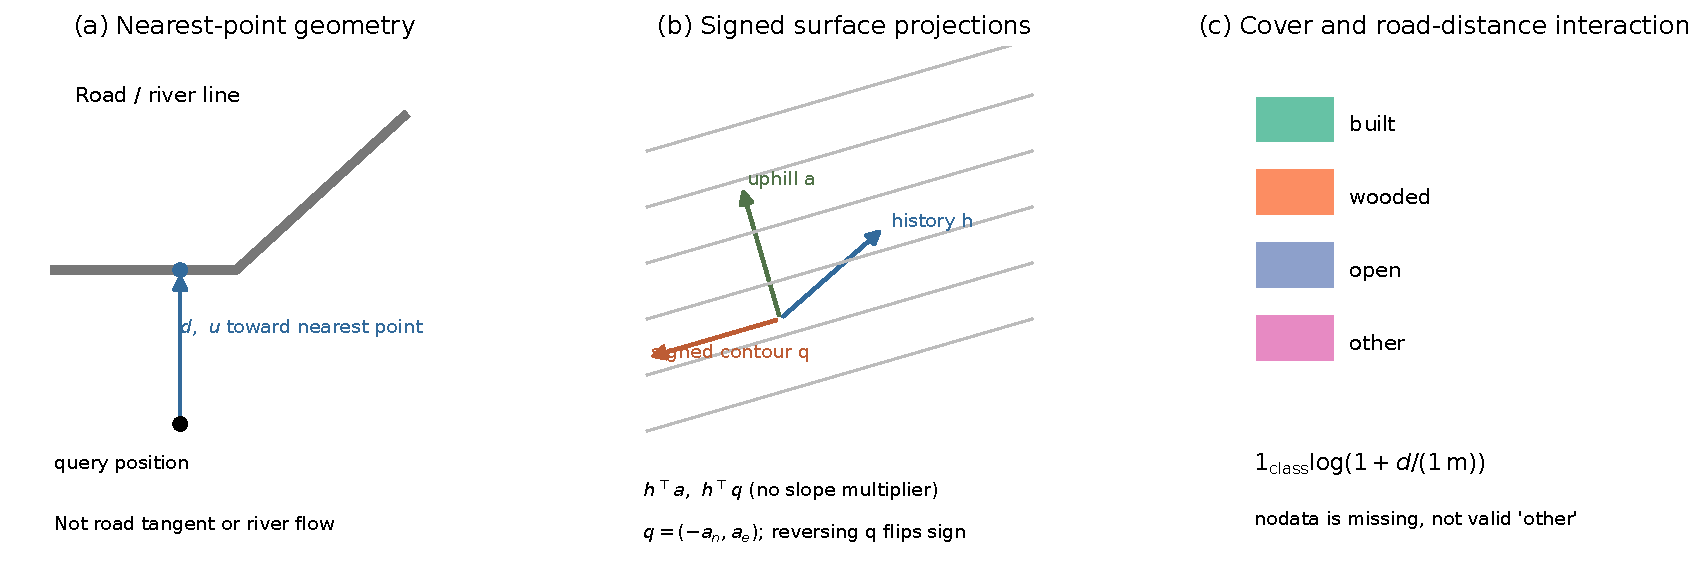
\includegraphics[width=\linewidth]{../figures/revision46-v1/revision46-geometry.pdf}
\caption{Schematic, not a real route. Left: nearest road/river point, distance
and direction toward that point, not a tangent or river flow. Centre: signed
history $h$, uphill $a$ and contour $q$, with distinct dot products and slope
magnitude. Right: cover membership and retained-road distance combine;
invalid queries are not the valid ``other'' cover class. The excluded road
classes are listed in the main paper.}\label{fig:terrain-geometry}\hypertarget{fig:terrain-geometry}{}
\end{figure}
\begin{figure}[htbp]\centering
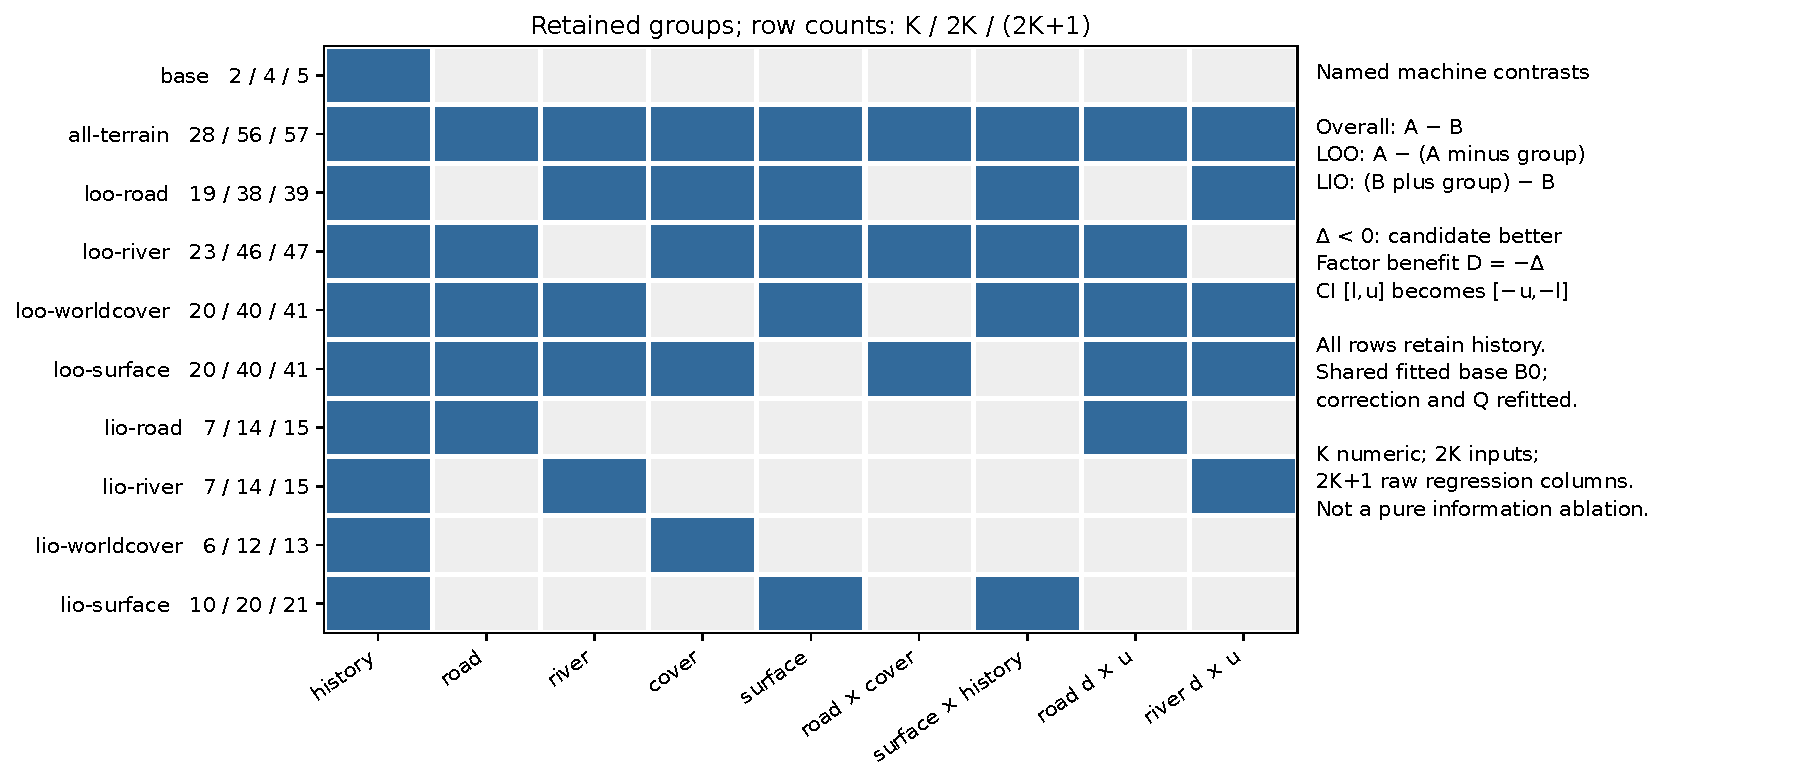
\includegraphics[width=\linewidth]{../figures/revision46-v1/revision46-design-matrix.pdf}
\caption{Ten independently fitted configurations. Road--cover interactions
require both parents; surface--history remains in LIO-surface. $K$ counts
numeric features, not total design columns. For LOO the machine candidate
is all-terrain and control is all-minus-group; a factor benefit expressed
as removal loss reverses the sign and interval endpoints. LIO compares
history-plus-group to base. The families and nonadditive interactions are
not redefined by this drawing.}\label{fig:terrain-matrix}\end{figure}
\FloatBarrier

\section{Complementary error and uncertainty views}
\begin{figure}[htbp]\centering
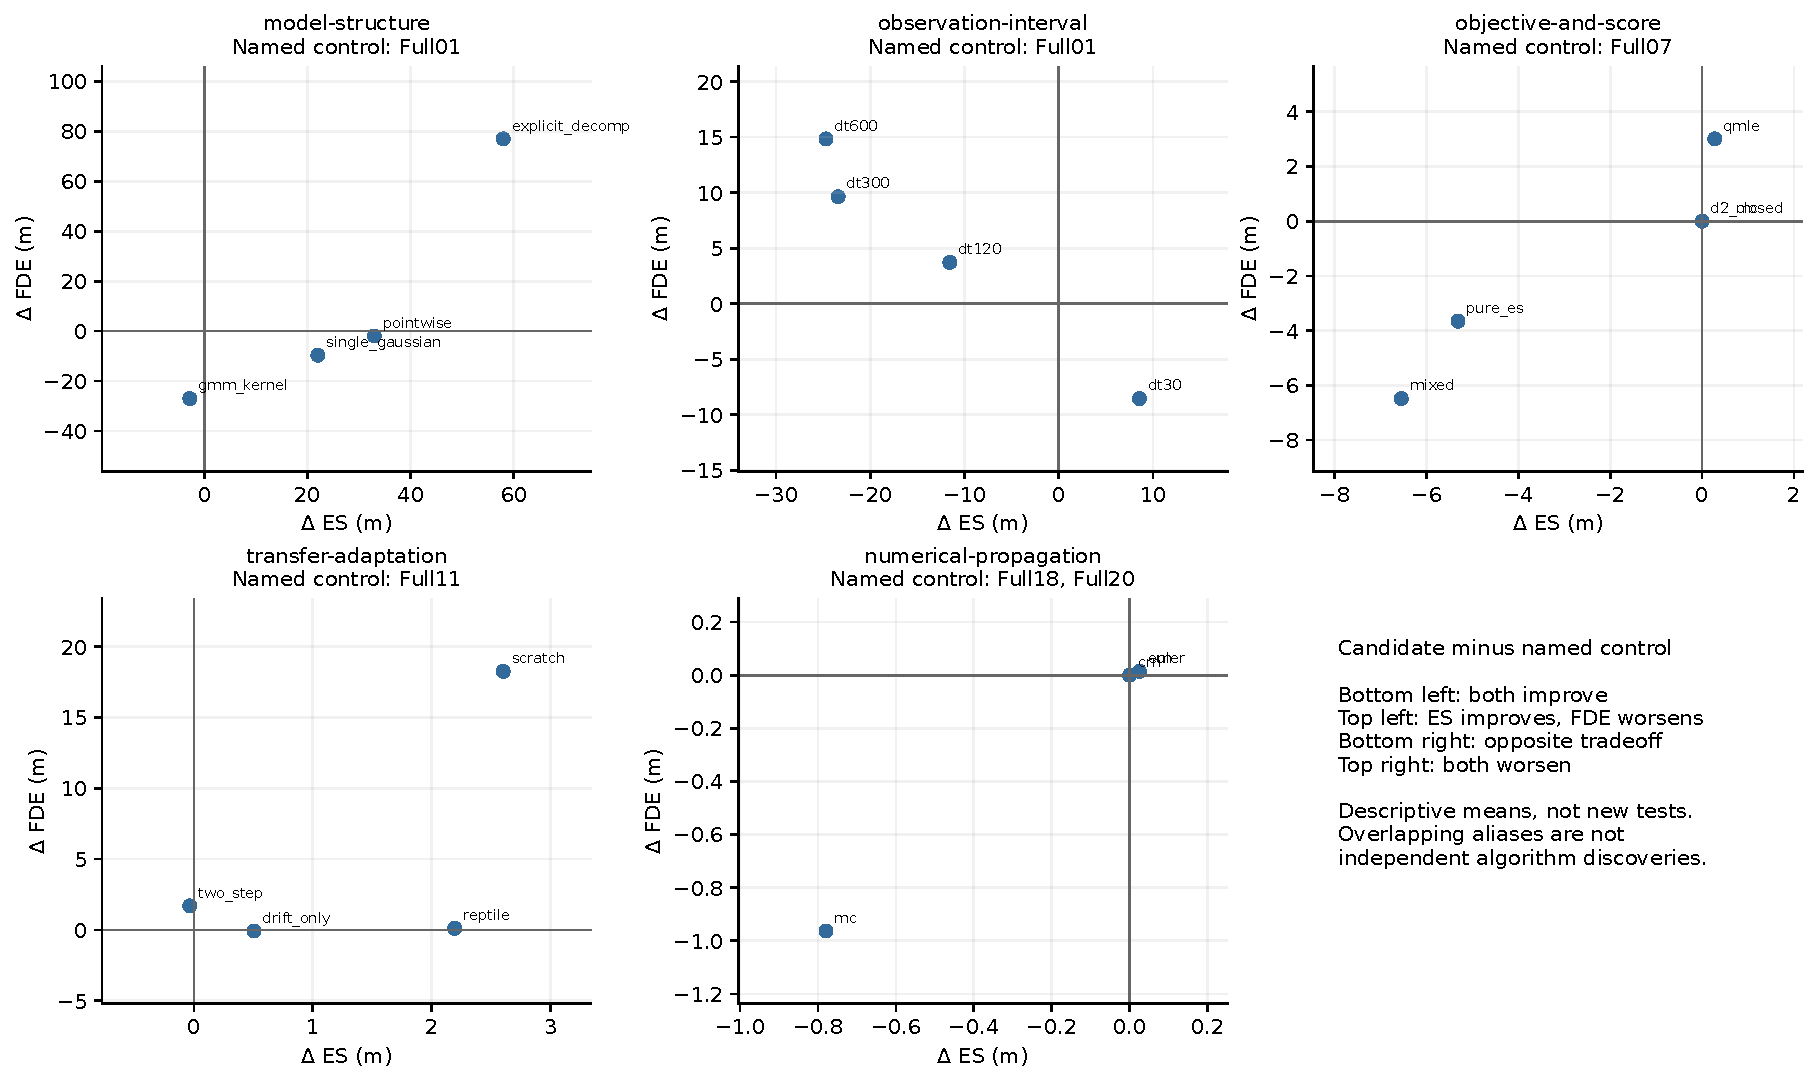
\includegraphics[width=\linewidth]{../figures/revision46-v1/revision46-score-error-tradeoff.pdf}
\caption{All 21 candidate-minus-named-control contrasts: weighted ES versus
mean-position FDE (m). Negative is favourable on each axis. Facets retain
original comparison families; named Full controls are not pooled. These
are descriptive paired means, not a new joint test or Pareto ranking.}
\label{fig:tradeoff}\end{figure}
\begin{figure}[htbp]\centering
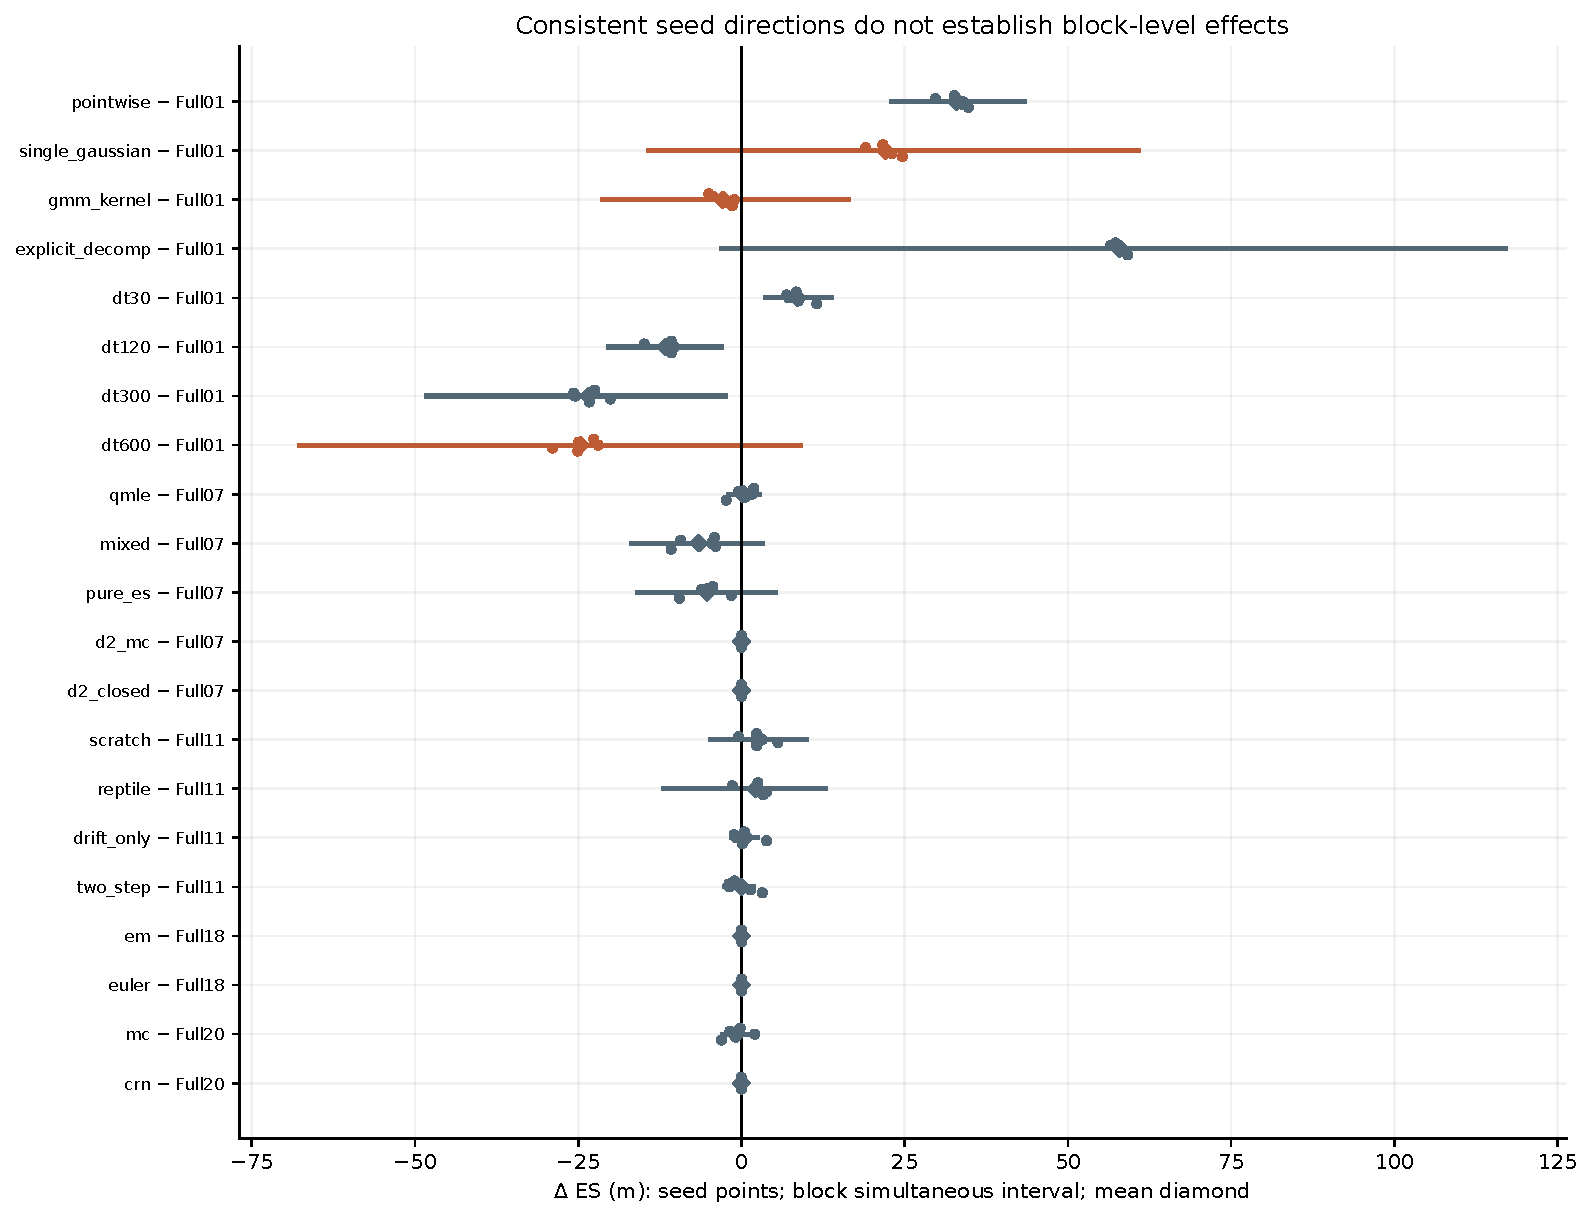
\includegraphics[width=\linewidth]{../figures/revision46-v1/revision46-seeds-and-blocks.pdf}
\caption{Five saved seed effects versus original record-block simultaneous
intervals (m). All comparisons are retained, including the examples with
unanimous seed signs and block intervals crossing zero. Seeds vary Monte
Carlo simulation, not fitted training samples or independent participants.}
\label{fig:seed-blocks}\end{figure}
\begin{figure}[htbp]\centering
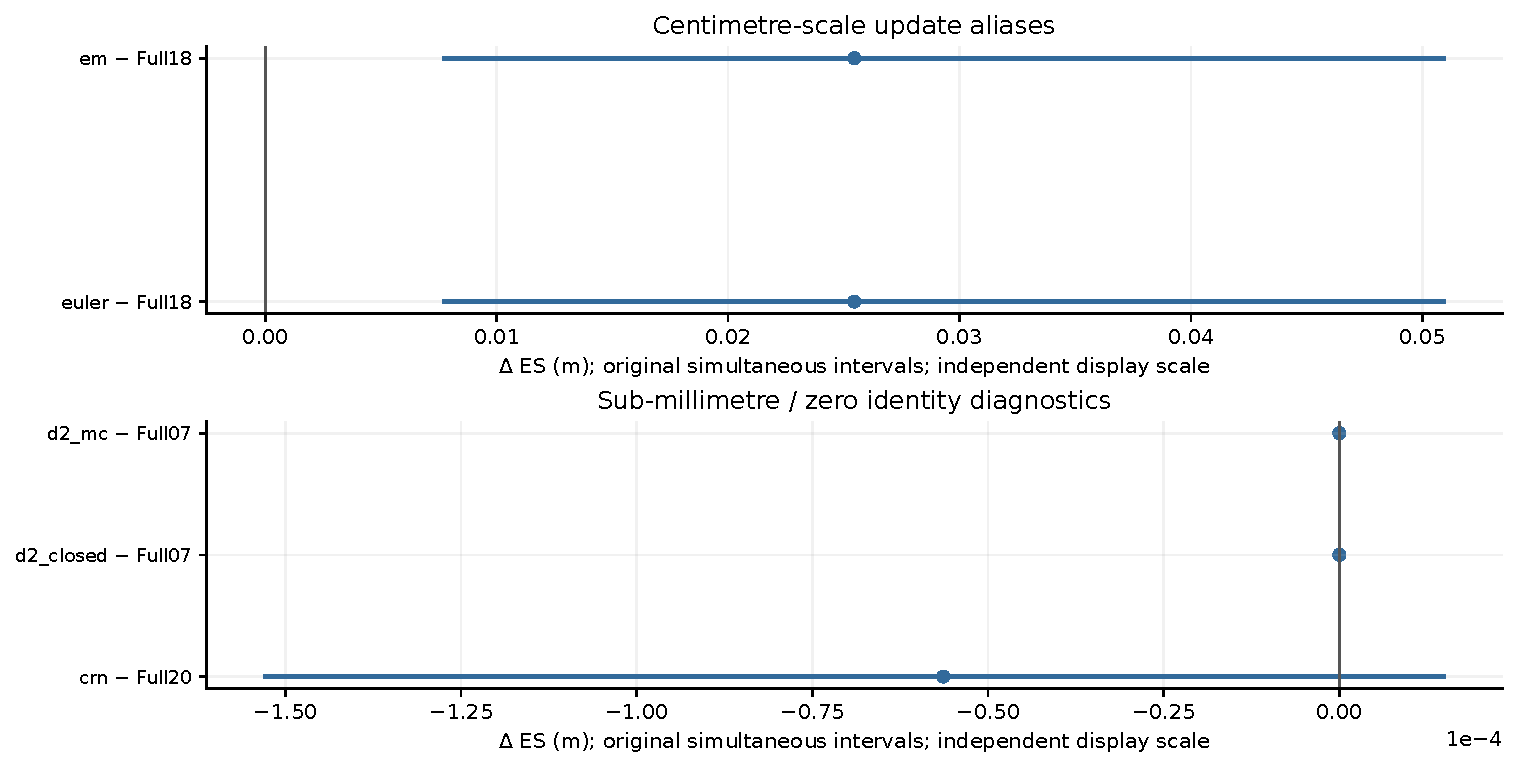
\includegraphics[width=\linewidth]{../figures/revision46-v1/revision46-identity-diagnostics.pdf}
\caption{Tiny implementation-consistency effects at their own explicitly
labelled scale, supplementing the main paper's practical-effect forest.
Original point estimates and intervals are unchanged; exact or near-zero
effects do not supply an independent power proof.}\label{fig:micro-effects}\end{figure}
\FloatBarrier

\section{Fit diagnostics, runtime and the complete method overview}
\begin{figure}[htbp]\centering
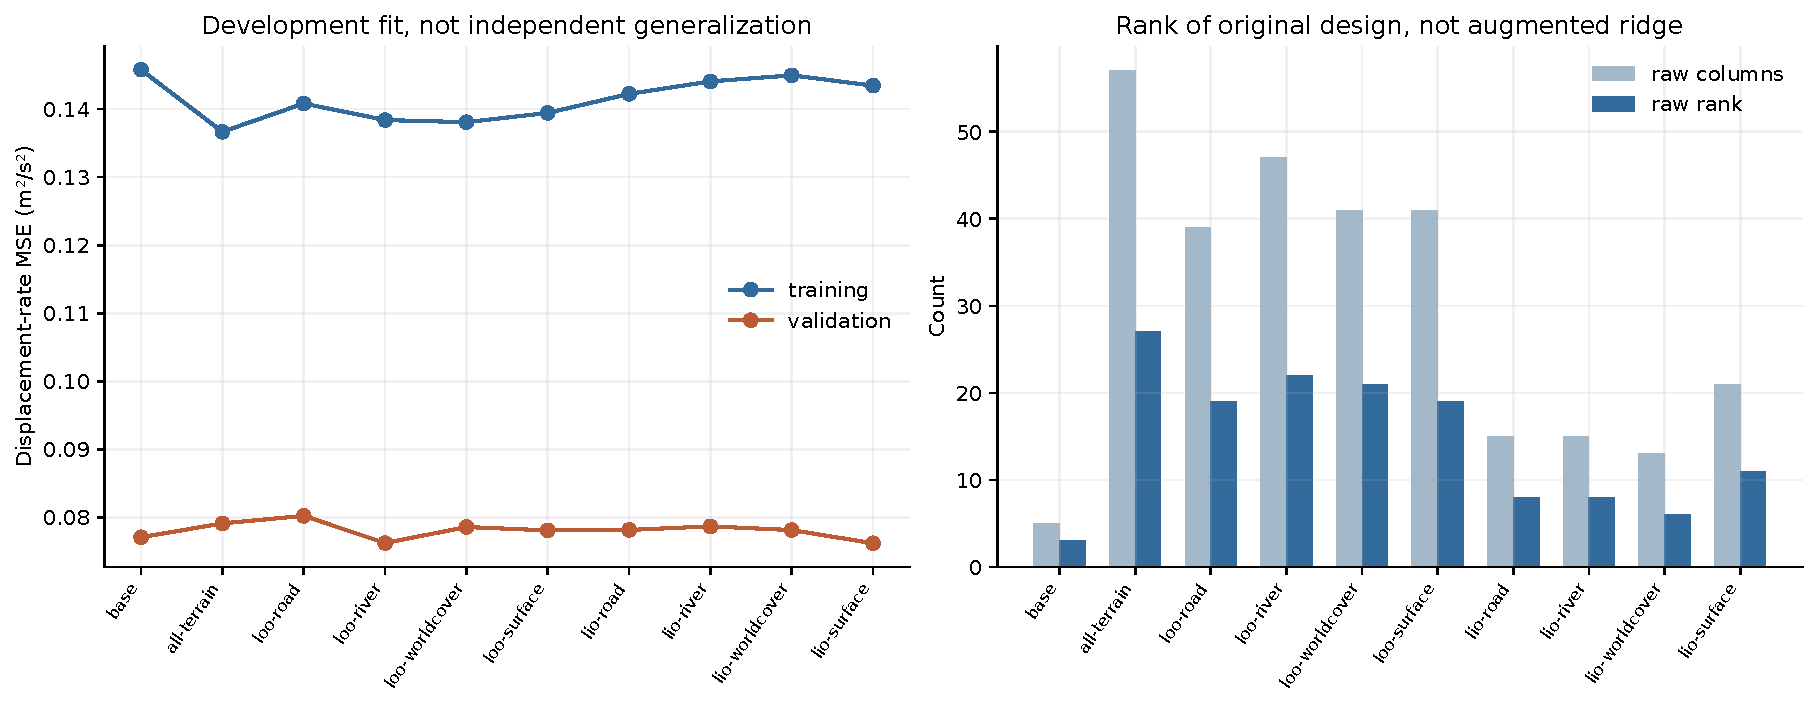
\includegraphics[width=\linewidth]{../figures/revision46-v1/revision46-development-fit.pdf}
\caption{Ten development configurations: training/validation displacement-rate
MSE (m$^2$/s$^2$), original columns and raw rank. Fit error is not forecast
ES. Raw rank deficiency, augmented-ridge full rank and out-of-sample
performance are distinct. Rows and regularisation remain unchanged.}
\label{fig:fit-diagnostics}\end{figure}
\begin{figure}[htbp]\centering
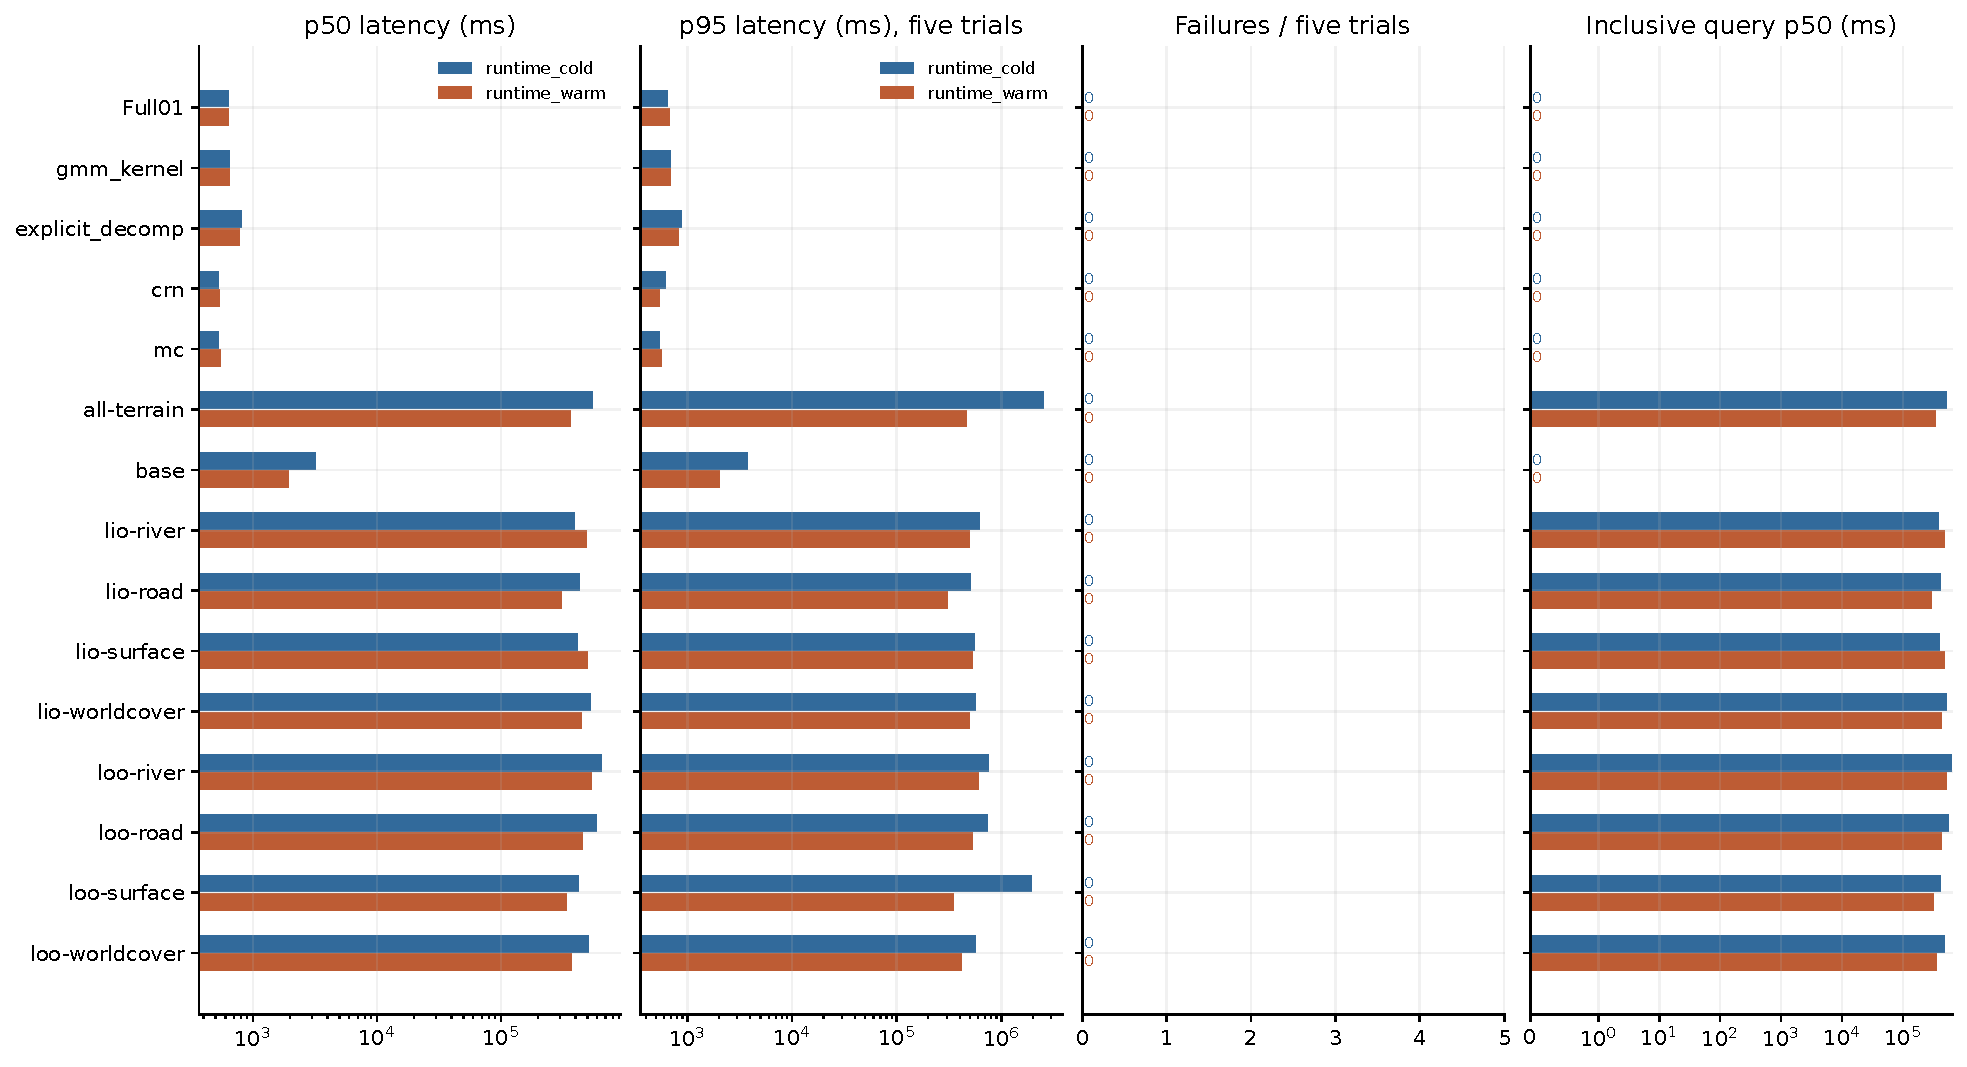
\includegraphics[width=\linewidth]{../figures/revision46-v1/revision46-recorded-runtime.pdf}
\caption{Completed original provider-cold/provider-warm latency p50/p95
(ms) and failure counts for all 15 subjects. Each condition uses five trials;
15 prewarm runs are excluded from quantiles, not the recorded exposed trials.
Provider-cold is not OS-cache-cold. Query costs are inclusive in rollout;
five observations do not estimate a stable operational tail.}\label{fig:runtime}\end{figure}
\FloatBarrier
\begin{figure}[p]\centering
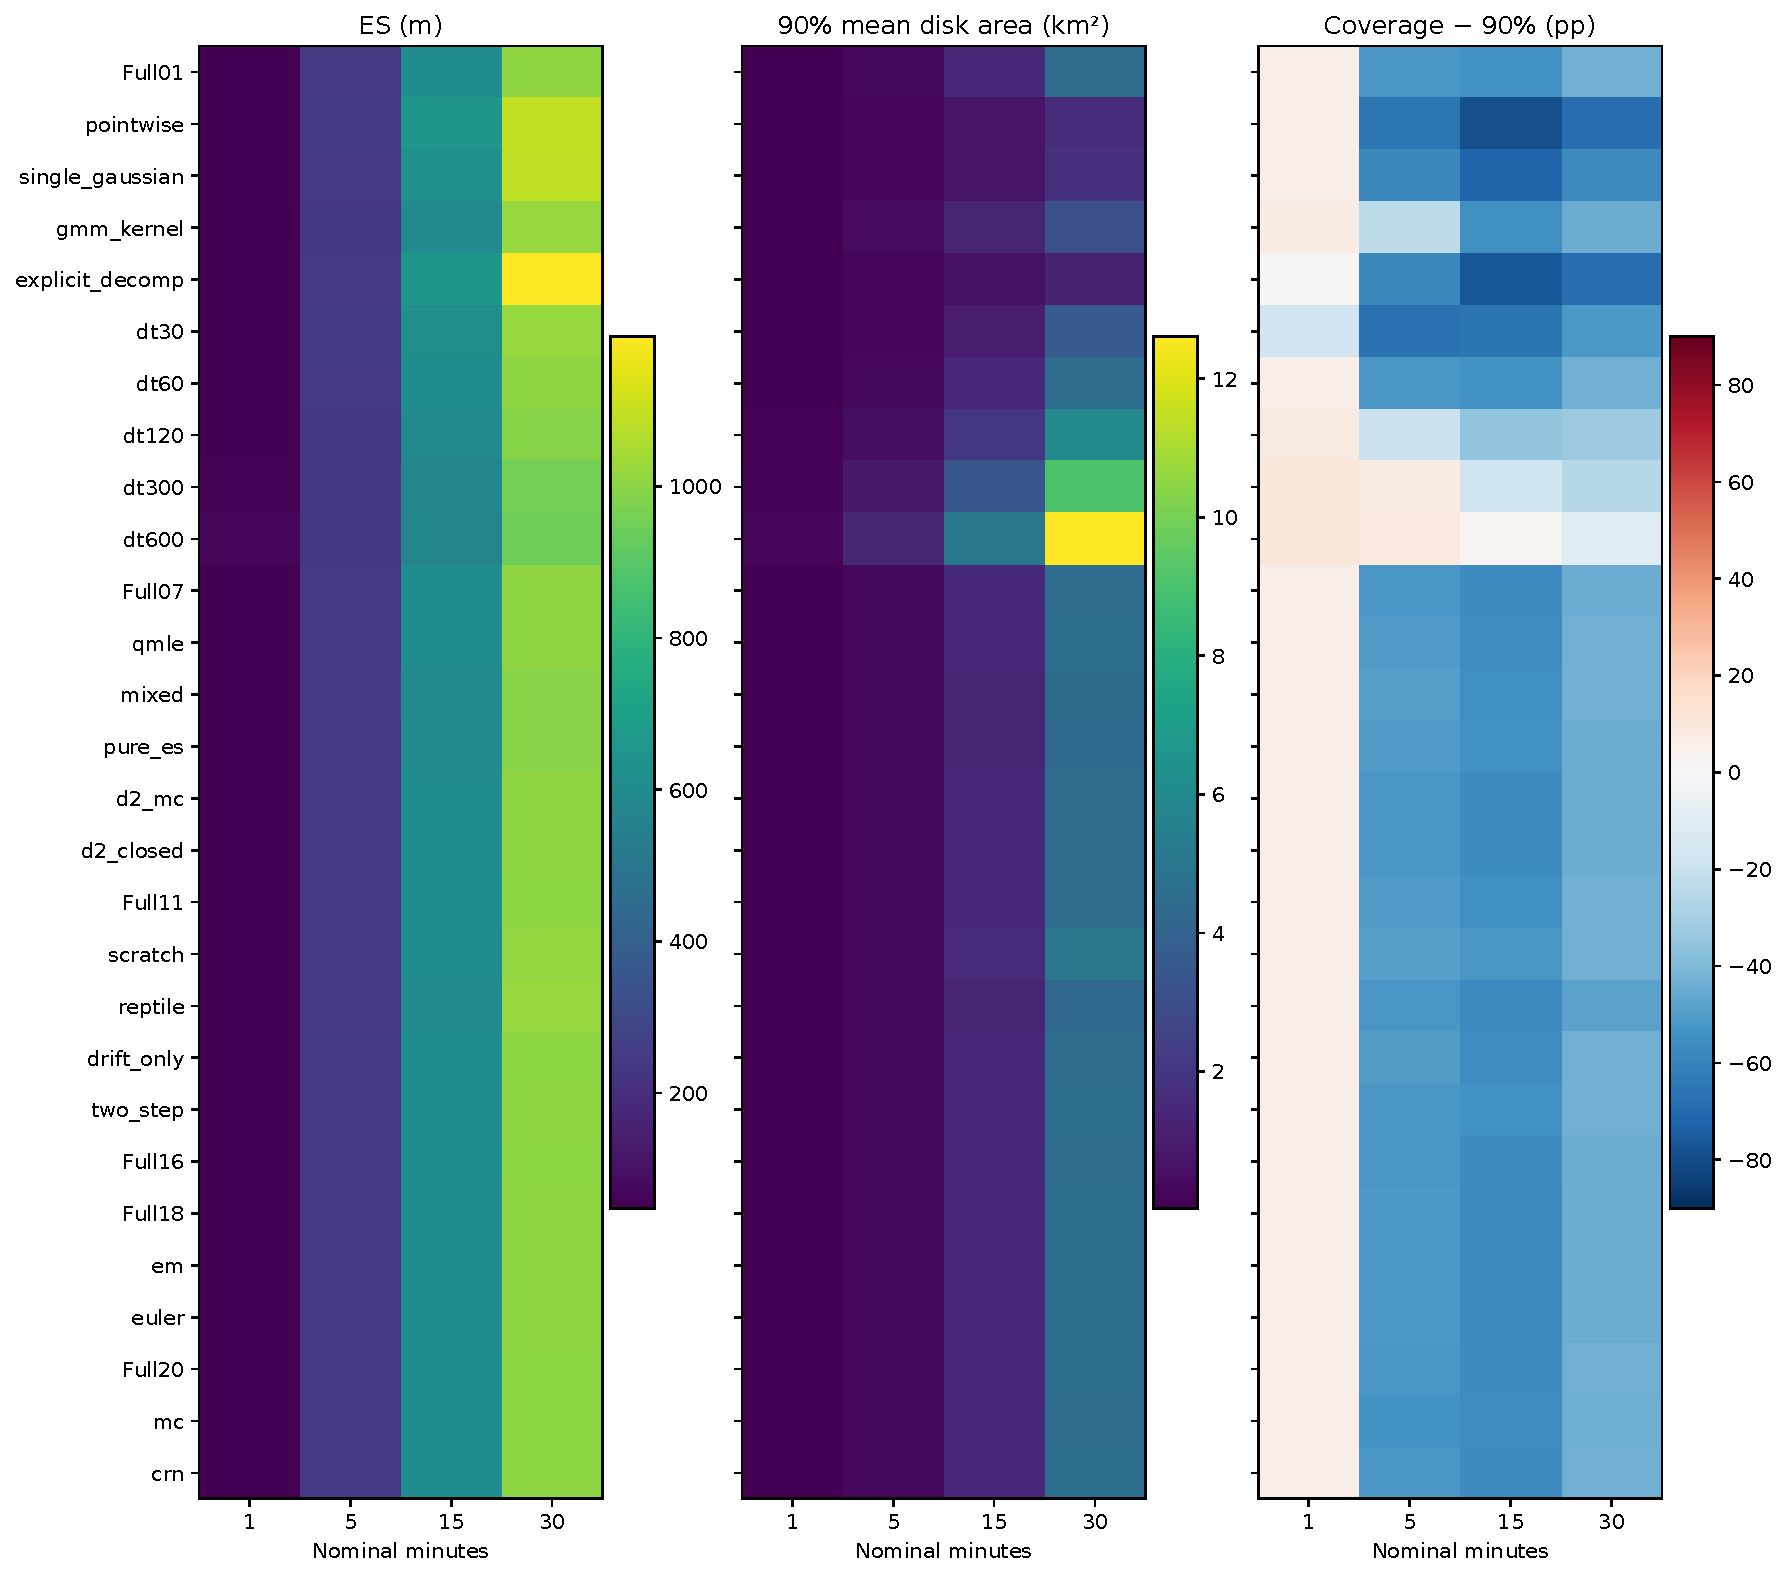
\includegraphics[width=\linewidth,height=.83\textheight,keepaspectratio]{../figures/revision46-v1/revision46-metric-overview.pdf}
\caption{All 28 saved method identities and four horizons: ES (m), mean 90\%
disk area (km$^2$), and coverage minus nominal 90\% (percentage points).
The shared diverging coverage scale is centred at zero, with both
overcoverage and undercoverage visible. Complete all-level tables remain
below; no configuration is selected as a winner.}\label{fig:method-overview}\hypertarget{fig:method-overview}{}
\end{figure}\FloatBarrier

\section{Family availability, not a terrain benefit ranking}
\begin{figure}[htbp]\centering
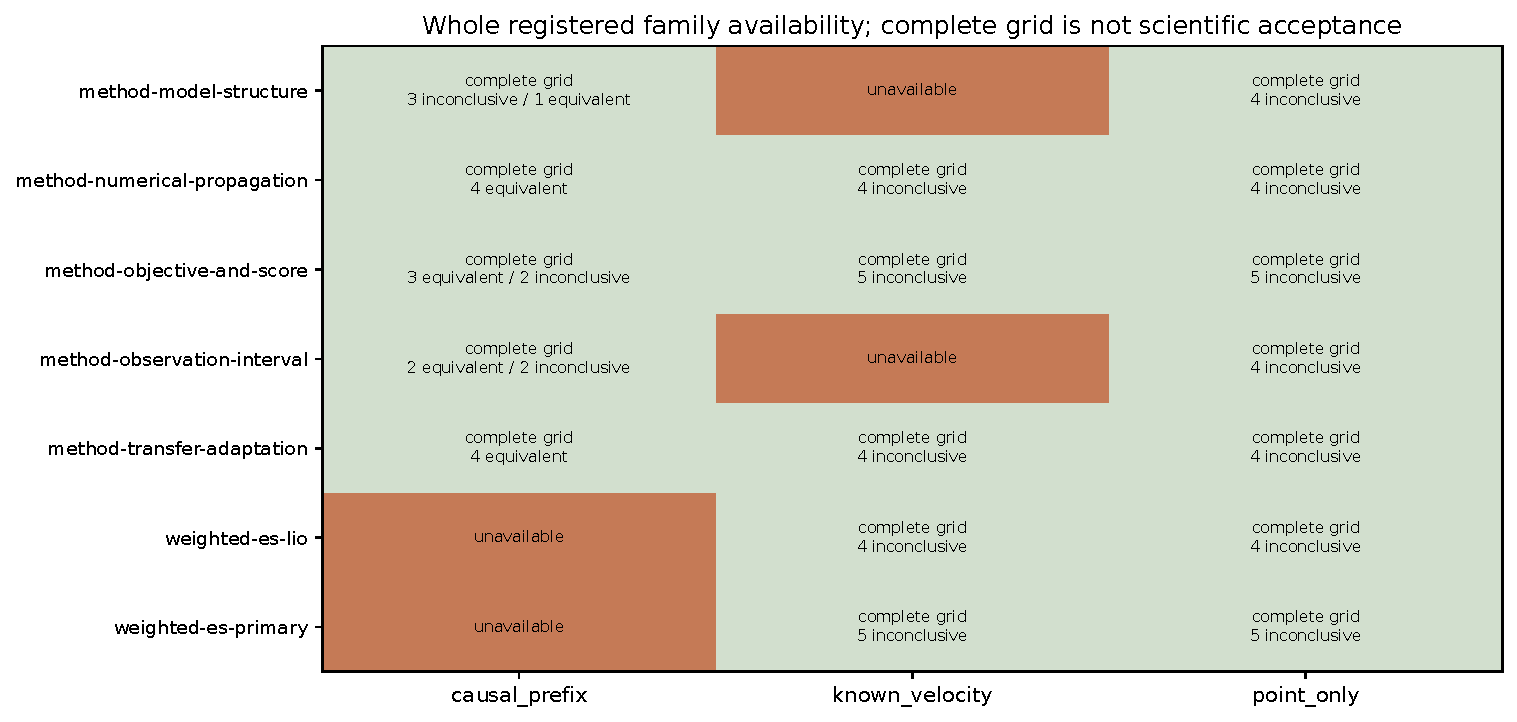
\includegraphics[width=\linewidth]{../figures/revision46-v1/revision46-family-availability.pdf}
\caption{Original seven families by three origin modes. A required failure
invalidates its whole registered family; individual successful pairs are
not a replacement family. Complete does not mean accepted, practically
beneficial, mechanism-qualified or resolution-invariant. The original
comparison tables retain each qualification reason.}\label{fig:availability}\hypertarget{fig:availability}{}
\end{figure}\FloatBarrier

\section{Missing-input and history-feedback limits}
Invalid online numeric features are zero-filled with a validity mask.
Within a frozen conditioner, the induced drift change is
$\Delta b=\theta_{\rm num}\Delta f+\theta_{\rm mask}\Delta m$, not necessarily zero.
The 404/81 valid development origins do not span these missing-input states.
Feature-file counts, cached query counts, absence of an element, invalid
geometry and a failed forecast have different denominators. Full early/late
speed and drift traces and per-feature missingness across every forecast
were not retained; the four position snapshots cannot reconstruct them.
A one-half overlap correlation for constant-noise 10 s secants is a local
calculation, not evidence for the full nonlinear feedback process or a
measured observation-noise model. No long simulations are rerun here.

\section{Retained detailed scientific specifications and tables}
The following mechanically migrated units retain the original formulas,
tables and source identities. Their unit-level hashes and old-label
destinations are recorded in \path{revision46-source-migration.json};
the verbatim pre-revision files remain separately named historical sources.
Only reading structure, cross-document links and counting-unit clarification
are changed. The main paper, not an older snapshot's pending wording,
determines the current review state.
\section{Related work and scope}\label{sec:related-work}\hypertarget{sec:related-work}{}

\section{Continuous-time motion and switching dynamics}
Persistent motion has a well-established stochastic formulation. Johnson
et al.\ integrate an Ornstein--Uhlenbeck velocity process to obtain a
continuous-time correlated random walk for irregular animal telemetry,
including a state-space observation model\cite{johnson2008}. The connection
is temporal persistence and a distribution over future locations. Here the
propagated continuous state is position; velocity and heading summaries are
constructed from the visible prefix and, where enabled, simulated history.
We do not estimate the same latent-velocity and observation-error model.
The animal-telemetry application is a methodological precedent, not evidence
that its population or observation process matches these GPX recordings.

Ghahramani and Hinton combine discrete regimes with linear continuous
dynamics in switching state-space models and use variational inference for
otherwise intractable hidden-state posteriors\cite{ghahramani2000}.
This establishes why locally Gaussian dynamics need not produce a single
Gaussian trajectory distribution. Our fitted modes and conditional
propagators use that broader modelling idea, but ordinary mode weights are
saved fit parameters rather than a newly inferred prefix posterior. The
specific fitting, switching and propagation rules are described below;
neither a mixture nor a switching mechanism is claimed as a new invention.


\section{Environment-conditioned and learned dynamics}
Environmental information can enter movement models through more than a
map image. Integrated step selection analysis jointly estimates movement
and resource-selection parameters by comparing observed steps with
available alternatives\cite{avgar2016}. Its corrected parameter expressions
are documented separately\cite{avgar2017correction}; we use the framework
only for conceptual positioning, not its likelihood or coefficient formulas.
Our road, river, cover and surface features instead modify a position-SDE
drift. The terrain comparisons ask about incremental predictive information
after refitting within a fixed feature family, not habitat preference or a
causal effect of landscape on behaviour.

Neural SDEs enlarge the function class, but their learning tasks differ.
Kidger et al.\ use Brownian input to generate paths with an SDE solver and
train against a neural controlled differential-equation discriminator in
a Wasserstein-GAN formulation\cite{kidger2021}. Gao et al.'s Langevin Graph
Network Approach (LaGNA) instead targets equations for coupled network
dynamics, separating self, interaction and diffusion contributions with
neural modules\cite{gao2024}. Generating a path distribution and recovering
a governing network equation are distinct objectives. Our single-record
GPX task evaluates finite position forecasts; it does not identify
inter-agent interaction laws or validate recovered equations against known
ground truth. Social GAN couples recurrent motion histories,
inter-agent pooling and adversarial diversity\cite{gupta2018}.
Trajectron++ combines probabilistic multi-agent forecasting, dynamics and
heterogeneous context including semantic maps\cite{salzmann2020}.
These works connect multimodality, dynamics and context, but address
different data, interaction structures and training objectives.

We retain the previously selected linear-in-parameters conditioner to make
the feature definitions and matched component changes inspectable.
This is a fixed representation choice, not evidence that linear models
are optimal. Gaussian-mixture modes, history feedback and spatial features
also mean that linear coefficients do not imply one globally linear,
single-Gaussian path law. The present contribution is the controlled study
of method components and environmental inputs in one visible-prefix GPX
task, including their limitations; it is not a new neural architecture.
The cited external models are not executed baselines. The registered simple
inertial reference now has a descriptive same-population comparison in
Section~\ref{sec:inertial-primary}. This is not an independently audited
superiority claim, and no superiority over the cited external models follows.


\section{Distributional evaluation and finite-computation evidence}
A predictor must be assessed as a distribution, not only by the distance
between its mean and a realized endpoint. Proper scoring rules provide
this foundation\cite{gneiting2007,gneiting2008}. We use a common energy-score
estimator alongside mean-position error, empirical coverage and region
size: a larger region may cover more outcomes without improving location
accuracy. Component effects therefore require paired comparisons and an
explicit practical-importance threshold, not a ranking of isolated scores.

Numerical integration and ensemble sampling add distinct approximation
errors\cite{kloeden1992}; increasing particles does not increase the number
of recording blocks. Our finite numerical evidence is reported separately
from block uncertainty. Familywise confidence intervals use a studentized
block bootstrap\cite{davison1997}, whereas Holm adjustment concerns
zero-null test probabilities\cite{holm1979}. Adaptation is described by the
executed first-order Reptile-style updates\cite{nichol2018}.
Together these distinctions define what the existing comparisons can
support without converting a finite check into a convergence theorem,
a confidence interval into a test probability, or training diagnostics
into held-out predictive performance.


\section{Forecast models and terrain ownership}
\label{sec:models}\hypertarget{sec:models}{}
Figure~\ref{fig:model-data-flow} separates the two executed model families
before introducing their equations. Both predict future positions; neither
predicts a future map. Static geographic features enter the terrain branch,
whereas the ordinary method Full uses local position, solar elevation and
sampled modes, not the terrain regression. Their common scoring protocol
does not make them one fitted model or one interchangeable control.
\paragraph{Terminology.}
A terrain \emph{conditioner} is the additive drift correction
\(c_{\theta_g}(F_g)\), not a separate likelihood or neural network.
A \emph{provider} returns map or clock features; an \emph{ensemble} is a
collection of simulated forecast paths, not independent observations.
A \emph{verdict} is an evidence disposition under the registered rules,
not a model ranking. \texttt{Full} denotes the ordinary method reference,
whereas \texttt{base} and \texttt{all-terrain} denote terrain configurations.
Code identifiers remain unchanged. In particular, \texttt{dt} labels an
observation interval, not the integration step, and \texttt{two\_step} and
\texttt{explicit\_decomp} are separate implemented alternatives.
\begin{figure}[p]
\centering
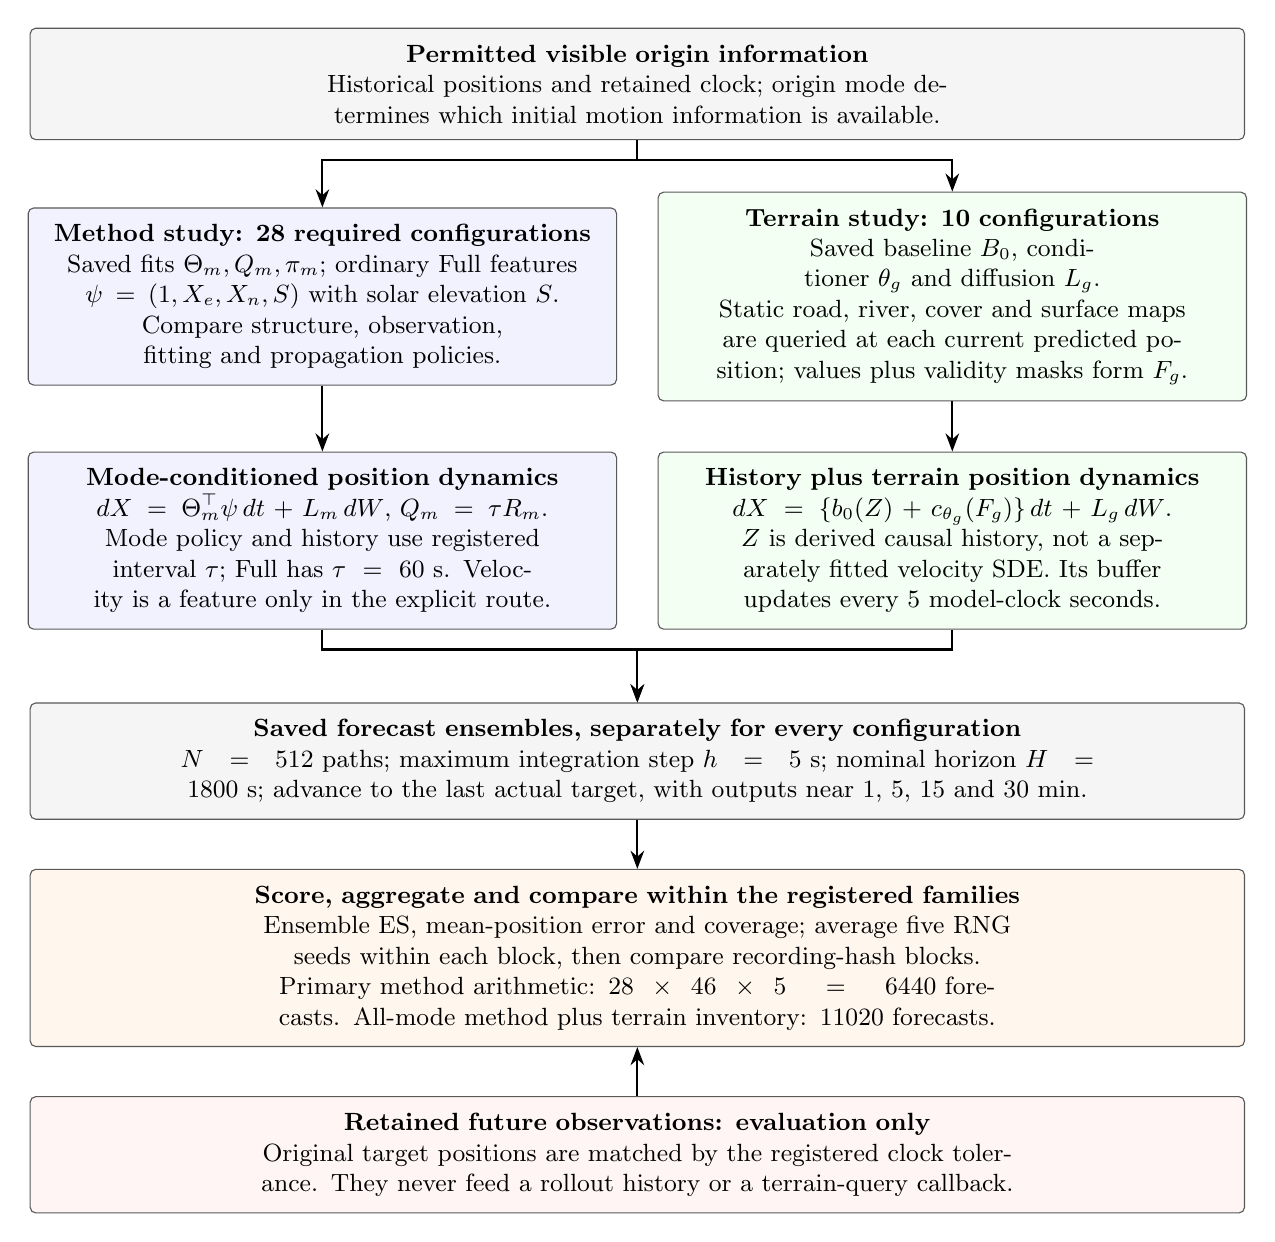
\begin{tikzpicture}[
  box/.style={draw=black!65,rounded corners=2pt,align=center,
    font=\small,inner sep=6pt},
  branch/.style={box,text width=7.05cm,minimum height=1.8cm},
  wide/.style={box,text width=15cm,minimum height=1.1cm},
  flow/.style={-{Stealth[length=2.3mm]},thick}]
\node[wide,fill=black!4] (origin) at (0,0)
  {\textbf{Permitted visible origin information}\par
  Historical positions and retained clock; origin mode determines
  which initial motion information is available.};
\node[branch,fill=blue!5] (method) at (-4,-2.7)
  {\textbf{Method study: 28 required configurations}\par
   Saved fits $\Theta_m,Q_m,\pi_m$; ordinary Full features
  $\psi=(1,X_e,X_n,S)$ with solar elevation $S$.\par
  Compare structure, observation, fitting and propagation policies.};
\node[branch,fill=green!5] (terrain) at (4,-2.7)
  {\textbf{Terrain study: 10 configurations}\par
  Saved baseline $B_0$, conditioner $\theta_g$ and diffusion $L_g$.\par
  Static road, river, cover and surface maps are queried at each
  current predicted position; values plus validity masks form $F_g$.};
\node[branch,fill=blue!5,minimum height=2cm] (mdyn) at (-4,-5.8)
  {\textbf{Mode-conditioned position dynamics}\par
  $dX=\Theta_m^\top\psi\,dt+L_m\,dW$, $Q_m=\tau R_m$.\par
  Mode policy and history use registered interval $\tau$;
   Full has $\tau=60$ s. Velocity is a feature only in the explicit route.};
\node[branch,fill=green!5,minimum height=2cm] (tdyn) at (4,-5.8)
  {\textbf{History plus terrain position dynamics}\par
  $dX=\{b_0(Z)+c_{\theta_g}(F_g)\}\,dt+L_g\,dW$.\par
  $Z$ is derived causal history, not a separately fitted velocity SDE.
  Its buffer updates every 5 model-clock seconds.};
\node[wide,fill=black!4] (output) at (0,-8.6)
  {\textbf{Saved forecast ensembles, separately for every configuration}\par
  $N=512$ paths; maximum integration step $h=5$ s; nominal horizon
   $H=1800$ s; advance to the last actual target, with outputs near
   1, 5, 15 and 30 min.};
\node[wide,fill=orange!7,minimum height=1.6cm] (score) at (0,-11.1)
  {\textbf{Score, aggregate and compare within the registered families}\par
  Ensemble ES, mean-position error and coverage; average five RNG seeds
  within each block, then compare recording-hash blocks.\par
  Primary method arithmetic: $28\times46\times5=6440$ forecasts.
  All-mode method plus terrain inventory: $11020$ forecasts.};
\node[wide,fill=red!4] (truth) at (0,-13.6)
  {\textbf{Retained future observations: evaluation only}\par
  Original target positions are matched by the registered clock tolerance.
  They never feed a rollout history or a terrain-query callback.};
\draw[flow] (origin.south) -- ++(0,-.25) -| (method.north);
\draw[flow] (origin.south) -- ++(0,-.25) -| (terrain.north);
\draw[flow] (method) -- (mdyn);
\draw[flow] (terrain) -- (tdyn);
\draw[flow] (mdyn.south) -- ++(0,-.25) -| (output.north);
\draw[flow] (tdyn.south) -- ++(0,-.25) -| (output.north);
\draw[flow] (output) -- (score);
\draw[flow] (truth) -- (score);
\end{tikzpicture}
\caption{Executed-model and evaluation data flow, not an additional
experiment or a neural architecture. The two branches have independent
fitted models and controls. The future-observation arrow ends at scoring,
not prediction. $\tau$ (observation/history interval), $h$ (integration
step) and $H$ (forecast duration) are distinct; $N$ and five RNG seeds
are simulation resources, not independent observed people. The nominal
time axis is conditional on retained clock provenance.}
\label{fig:model-data-flow}\hypertarget{fig:model-data-flow}{}
\end{figure}

\section{Causal terrain dynamics}
The prediction target is a distribution of future positions conditional on
the visible origin, not a separate prediction of terrain or a measured
future velocity. Let \(X_t=(X_{t,e},X_{t,n})^\top\in\R^2\) be east/north
position in metres. Let \(Z_t\) collect the causal position-history buffer,
its secant velocity \(v_t\) (metres per second), unit direction \(h_t\),
and direction-validity flag \(\eta_t\). These auxiliary quantities are
computed from visible positions initially and predicted positions thereafter;
\(Z_t\) has no independently fitted velocity SDE. A static map lookup at
the current \(X_t\), combined with this history, is encoded as
\(F_g(X_t,Z_t)=\phi_g\in\R^{2K_g}\), including values and masks.
Here \(g\) denotes a selected terrain configuration, not a latent mode.
The terrain predictor evolves as
\begin{equation}
 dX_t=\{b_0(Z_t)+c_\theta(F_g(X_t,Z_t))\}\,dt+L\,dW_t .
 \label{eq:terrain-sde}\hypertarget{eq:terrain-sde}{}
\end{equation}
\(W_t\in\R^2\) is a standard Wiener process with independent components,
\(\operatorname{Cov}(W_{t+\Delta}-W_t)=\Delta I_2\).
The drift \(b_0+c_\theta\) has units of metres per second;
\(L\in\R^{2\times2}\) is a constant noise-amplitude matrix with units
metres per square-root second. Its covariance is \(Q=LL^\top\), not \(L\)
itself. The two deterministic parts are explicitly
\begin{equation}
 \begin{aligned}
 r(Z_t)&=(1,v_{t,e},v_{t,n},\|v_t\|,h_{t,e},h_{t,n},\eta_t)^\top,\\
 b_0(Z_t)&=B_0^\top r(Z_t),\qquad
 c_\theta(\phi_g)=\theta^\top(\phi_g^\top,1)^\top .
 \end{aligned}
 \label{eq:drift-components}\hypertarget{eq:drift-components}{}
\end{equation}
Here \(B_0\in\R^{7\times2}\) fits the baseline displacement rate by
ridge regression with strength \(10^{-6}\); invalid history direction
components are zero with \(\eta_t=0\).
Writing \(R\) for the stacked rows \(r(Z_i)^\top\) and \(V_i=\Delta x_i/\Delta t_i\),
the actual first-stage fit is
\begin{equation}
 B_0=\arg\min_B\{\|RB-V\|_F^2+\rho\|B\|_F^2\}
     =(R^\top R+\rho I_7)^{-1}R^\top V,\qquad\rho=10^{-6}.
 \label{eq:baseline-fit}\hypertarget{eq:baseline-fit}{}
\end{equation}
This is an unnormalized sum-of-squares objective, including a penalized
intercept; \(\rho\) is not a mean-loss penalty. The two stages are sequential,
not a joint optimization of \(B_0\) and \(\theta\). All ten saved terrain fits
have exactly identical \(B_0\) coefficients; only the selected correction
design and fitted diffusion differ. This check compares existing parameters,
not a new fit or a claim that the correction is orthogonal to history.
The conditioner coefficients \(\theta\in\R^{(2K_g+1)\times2}\)
include an intercept. They fit the residual left by the baseline, rather than
regressing observed position directly on a map label.
For training transition \(i\), define
\(y_i=\Delta x_i/\Delta t_i-b_0(Z_i)\) and
\(x_{{\rm aug},i}=(\phi_{g,i}^\top,1)\).
Stacking the rows gives \(Y\in\R^{n\times2}\) and
\(X_{\rm aug}\in\R^{n\times(2K_g+1)}\).
Each conditioner solves
\begin{equation}
 \min_\theta\frac{1}{2n}\|X_{\rm aug}\theta-Y\|_F^2
       +\frac{\lambda}{2}\|\theta\|_F^2,\qquad\lambda=10^{-4},
 \label{eq:conditioner-fit}\hypertarget{eq:conditioner-fit}{}
\end{equation}
The first term is the mean squared residual over \(2n\) scalar outputs;
\(\|\cdot\|_F^2\) sums their squared entries. The second penalizes large
coefficients, including the bias, to stabilize a correlated feature design.
The value of \(\lambda\) is frozen, not selected on final outcomes.
Augmented least squares implements this mean-squared objective in float64;
stationarity and conditioning checks accompany the fitted parameters.
For two outputs its normal equation is
\((X_{\rm aug}^\top X_{\rm aug}+n\lambda I)\theta=X_{\rm aug}^\top Y\).
At \(n=404\), the saved diagonal penalty is \(0.0404\), not \(10^{-4}\).
Thus the baseline and correction regularizers have different loss
normalizations; their numeric strengths cannot be compared directly.
Each qualified development window supplies one origin-to-first-future row.
Both regressions weight displacement-rate rows equally, without duration,
inverse-noise, block or participant weights. The observed gap
\(\Delta t_i\) varies; it is neither the method fitting interval \(\tau\)
nor the integration step. Table~\ref{tab:terrain-fit-intervals} gives its
original development distribution, with no regular-time resampling.

This is a linear-in-parameters model on fixed engineered features, with no
hidden neural layers. Its drift need not be affine in position: nearest-map
queries, log distances, cover indicators and history updates depend
nonlinearly or discontinuously on predicted state. Neither the fitted signs
nor a physical road-attraction law are imposed. An ablation tests predictive
increment under this model, not the universal causal effect of terrain.

The diffusion covariance is estimated from training displacement residuals:
\begin{equation}
 LL^\top=\frac{1}{n}\sum_{i=1}^n
 \frac{(\Delta x_i-\widehat b_i\Delta t_i)
       (\Delta x_i-\widehat b_i\Delta t_i)^\top}{\Delta t_i}.
 \label{eq:diffusion}\hypertarget{eq:diffusion}{}
\end{equation}
The residual \(e_i=\Delta x_i-\widehat b_i\Delta t_i\) estimates the
unexplained displacement. Under the frozen-drift Brownian approximation,
\(e_i\sim\mathcal N(0,Q\Delta t_i)\), so
\(e_i/\sqrt{\Delta t_i}\) has covariance \(Q\), in square metres per second.
This explains the division by \(\Delta t_i\) and the residual-moment estimate;
it is not a global likelihood claim for the nonlinear history-dependent path.
Equivalently, with rate residual
\(\zeta_i=\Delta x_i/\Delta t_i-\widehat b_i\),
\begin{equation}
 Q=\frac1n\sum_{i=1}^n\Delta t_i\zeta_i\zeta_i^\top.
 \label{eq:terrain-rate-Q}\hypertarget{eq:terrain-rate-Q}{}
\end{equation}
Unlike equal-row drift regression, this rate outer product includes duration.
Residuals are not centered again, and the denominator is \(n\), not a
degrees-of-freedom correction. This is a plug-in second moment after fitting
drift, not an unbiased estimator or joint drift--diffusion maximum likelihood.
An eigendecomposition \(Q=U\operatorname{diag}(\lambda_1,\lambda_2)U^\top\)
supplies \(L=U\operatorname{diag}(\sqrt{\max(\lambda_j,0)})\).
The saved terrain loader rejects a smallest eigenvalue below
\(-10^{-10}\,\mathrm{m}^2/\mathrm{s}\) and asymmetry above the absolute
tolerance \(10^{-12}\,\mathrm{m}^2/\mathrm{s}\). Only tolerated negative
roundoff is set to zero for the square root; no positive floor or jitter is
added. All ten saved terrain matrices are symmetric and strictly positive,
so none requires this clipping. These absolute thresholds differ from the
method branch's relative PSD rule; positivity is not forecast calibration.
Each terrain configuration fits its own selected correction columns and
diffusion parameters while retaining the shared baseline coefficients.
Identical deterministic parameters can be bound to separate forecast seed
labels, but this does not represent five independent training realizations.
The ten terrain fits and 16 distinct deterministic method fitting identities
are restored from saved models during continuation.

Euler--Maruyama integrates Equation~\eqref{eq:terrain-sde} with a maximum step
of 5 seconds and 512 particles. For substep \(\Delta\) and independent
\(\xi_k\sim\mathcal N(0,I_2)\), the implemented position update is
\begin{equation}
 X_{k+1}=X_k+\{b_0(Z_k)+c_\theta(F_g(X_k,Z_k))\}\Delta
             +\sqrt{\Delta}\,L\xi_k .
 \label{eq:terrain-update}\hypertarget{eq:terrain-update}{}
\end{equation}
This connects the drift to the conditional mean displacement and diffusion
to increment covariance \(Q\Delta\). History has its own 5-second model-clock cadence.
At each history tick, the predictor appends predicted positions and recomputes
its secant velocity. Between ticks, history and velocity remain fixed while
terrain queries use current predicted positions. Query callbacks have no
target trajectory container. Invalid feature values are numerically imputed
to zero and accompanied by explicit validity columns; invalid-query counts
remain part of the evidence.

The history operator is part of the model, not an integration detail.
At terrain tick \(t_j=5j\) seconds after the origin, let
\(\{(s_{j,r},x^{(p)}_{j,r})\}_{r=1}^{q_j}\), \(2\le q_j\le3\),
be particle \(p\)'s retained buffer after appending its new predicted position
and keeping at most three entries. Its velocity is
\begin{equation}
 v^{(p)}_{t_j}=\frac{x^{(p)}_{j,q_j}-x^{(p)}_{j,1}}
                         {s_{j,q_j}-s_{j,1}} .
 \label{eq:terrain-history}\hypertarget{eq:terrain-history}{}
\end{equation}
The initial buffer contains only the visible origin information permitted by
the origin mode. Early updates can therefore mix original irregularly timed
prefix points with predicted ticks; their denominator is the actual retained
time span, not an assumed 5 seconds. Once three equally spaced tick positions
are retained, the secant spans 10 seconds. Intermediate integration substeps
and requested scoring outputs do not themselves append history. Between
history ticks the retained buffer and velocity are held fixed.


\section{Observed and simulated history are different inputs}
\label{sec:history-feedback}\hypertarget{sec:history-feedback}{}
The terrain history is a three-position buffer, initialized with observed
positions and subsequently updated with generated positions at 5-second
model-clock ticks. If the last observed gap is \(d\), the first update
retains the last two observations and the new position, so the secant spans
\(d+5\) seconds. The second update retains the origin and the positions
at 5 and 10 seconds; subsequent spans are 10 seconds. A fixed number of
points therefore does not imply a fixed secant duration or unchanged
input distribution. The observed training, validation and primary-prefix
timings are reported separately in
Section~\ref{sec:empirical-history-timings}; they describe clock support,
not measured feedback velocities or an experiment changing this cadence.

There is also a noise-distribution change. For the illustrative local model
\(dX_t=b\,dt+L\,dW_t\) with constant \(b,L\), define a secant over \(T>0\):
\begin{equation}
 \widehat v_t=\frac{X_t-X_{t-T}}{T}
       =b+\frac{L(W_t-W_{t-T})}{T},\qquad
 \operatorname{Cov}(\widehat v_t)=\frac{Q}{T},
 \quad Q=LL^\top .
 \label{eq:secant-local-noise}\hypertarget{eq:secant-local-noise}{}
\end{equation}
Overlapping buffers reuse the same Brownian increments. For lag \(s\ge0\)
in this constant-coefficient illustration,
\begin{equation}
 \operatorname{Cov}(\widehat v_t,\widehat v_{t+s})
       =\frac{(T-s)_+}{T^2}Q .
 \label{eq:secant-overlap}\hypertarget{eq:secant-overlap}{}
\end{equation}
At \(T=10\), adjacent 5-second terrain ticks consequently have correlation
\(1/2\) in directions with nonzero variance, not independent velocity noise. The saved base and
all-terrain fits give \(\operatorname{tr}(Q)=2.7387\) and \(2.5077\)
\(\mathrm{m^2/s}\). The corresponding two-dimensional local RMS velocity
perturbations \(\sqrt{\operatorname{tr}(Q)/10}\) are \(0.5233\) and
\(0.5008\ \mathrm{m/s}\). These are arithmetic consequences of existing
diffusion fits, not measured rollout velocity dispersions or bounds for
the history-dependent model.

Observed GPX coordinates may also have measurement error. If one merely
illustrates independent endpoint errors of covariance \(R_{\rm obs}\),
independent of that local process, the observed-secant covariance becomes
\(Q/T+2R_{\rm obs}/T^2\). This is not a fitted sensor model: neither
\(R_{\rm obs}\) nor a zero-error observation assumption is established here.
Simulation instead feeds generated position increments back into both the
baseline velocity and history-dependent features. Normalizing direction,
changing map features and drift feedback invalidate the constant-drift
variance calculation as a formula for the complete predictor. The kernel
does not clip secant speed or apply a velocity-error filter at history ticks.
The six illustrated forecast archives retain four position outputs, not
full early/late velocity and drift traces. Thus the present evidence does
not identify history feedback as the cause of long-horizon undercoverage,
nor certify abnormal-speed rates or sensitivity to changing this cadence.
The method matrix uses its different adjacent-\(\tau\) secant
(Equation~\eqref{eq:method-history}); the 10-second calculation applies
to the terrain buffer only.


\section{Frozen terrain-feature encoding}
\label{sec:feature-encoding}\hypertarget{sec:feature-encoding}{}
The terrain conditioner uses the frozen pointwise transforms,
not a newly learned embedding or final-evaluation standardization. For road
and river, let \(d_g\) be the queried distance in metres and \(v_g\) the
query-supplied east/north unit vector from the query position towards the
nearest point on the selected polyline. The provider selects the closest
point in its local metric projection and reports a spherical distance to it.
Thus \(v_g\) is neither a line tangent, a road travel direction nor a river
flow direction; coincident queries have no usable direction. Their features are
\begin{equation}
 \ell_g=\log\{1+d_g/(1\,\mathrm{m})\},\qquad
 u_g=v_g/\|v_g\|,\qquad g\in\{\mathrm{road},\mathrm{river}\}.
 \label{eq:distance-encoding}\hypertarget{eq:distance-encoding}{}
\end{equation}
Distance is usable only when nonnegative. The unit-vector transform requires
a norm greater than \(10^{-12}\). Baseline history direction \(h\) uses the
same unit-vector transform, with availability determined by the causal
history/origin rules. These selected transforms have no fitted centering,
scaling or clipping parameters. The logarithm is a frozen engineering choice:
it preserves distance ordering, is finite at zero and compresses the large
range of map distances, with derivative \(1/(1\,\mathrm m+d_g)\).
These properties explain the representation, not its empirical optimality.
No physical logarithmic response law or comparison proving superiority to raw
distance is established by the present ablation; unselected transformations
remain outside its result claims.

The four WorldCover indicators \(w\) are, in order, built (code 50), vegetated
(10, 20, 30, 40, 95, 100), water/wetland (80, 90), and bare/snow/other (60, 70
or another finite unrecognized code). The last category applies only to a
usable source value: a missing or nodata query is not recoded as valid
``unknown'' cover. Surface orientation retains the six supplied components
\(s=(\beta,\sin\alpha,\cos\alpha,n_e,n_n,n_u)\): slope in radians, downslope
aspect east/north, and the three surface-normal components. This is an
identity transform, not a fitted terrain representation.

For a valid cover code \(k\), write
\begin{equation}
 \begin{aligned}
 w_j&=\mathbf1\{k\in\mathcal C_j\},\quad\mathcal C_1=\{50\},\\
 \mathcal C_2&=\{10,20,30,40,95,100\},\quad\mathcal C_3=\{80,90\},\\
 \mathcal C_4&=\R_{\rm finite}\setminus(\mathcal C_1\cup\mathcal C_2\cup\mathcal C_3).
 \end{aligned}
 \label{eq:cover-indicators}\hypertarget{eq:cover-indicators}{}
\end{equation}
This grouping cannot identify separate effects of buildings, individual
vegetation classes, wetland or snow. Absolute elevation \(H\) supplies surface
derivatives but is not itself a selected conditioner column. With the
east/north DEM gradient \(\gamma=(\partial_e H,\partial_n H)\), the geometric
definitions are
\begin{equation}
 \begin{aligned}
 \beta&=\arctan\|\gamma\|,\quad (\sin\alpha,\cos\alpha)=-\gamma/\|\gamma\|,\\
 (n_e,n_n,n_u)&=(-\gamma_e,-\gamma_n,1)/\sqrt{1+\|\gamma\|^2}.
 \end{aligned}
 \label{eq:surface-geometry}\hypertarget{eq:surface-geometry}{}
\end{equation}
The provider estimates gradients by central differences over DEM neighbours.
Aspect \(\alpha\) is clockwise from north and points downhill.
Flat terrain has no geometrically defined aspect: the provider records its
aspect vector as \((0,0)\), not an arbitrary northward direction. Thus a flat
surface's directional composition can be zero, without evidence of genuine
perpendicular travel. Masks still follow source-validity rules.

The four selected compositions are exactly
\begin{align}
 c_{\rm road}&=\ell_{\rm road}u_{\rm road},&
 c_{\rm river}&=\ell_{\rm river}u_{\rm river},\notag\\
 c_{\rm cover}&=\ell_{\rm road}w,&
 c_{\rm surface}&=(h^\top a,\ h^\top q),
 \label{eq:feature-compositions}\hypertarget{eq:feature-compositions}{}
\end{align}
where \(a=-(\sin\alpha,\cos\alpha)\) is uphill and
\(q=(-a_n,a_e)\) is the chosen contour direction. The surface composition
uses a positive 90-degree rotation of uphill in east/north coordinates.
There is one uphill direction and its opposite downhill direction, not two
distinct uphill choices. A contour has two orientations: the chosen \(q\)
fixes the sign convention and \(-q\) would reverse \(h^\top q\).
Positive \(h^\top a\) denotes uphill alignment; negative denotes downhill.
The signed contour projection distinguishes the two orientations but does
not give either an intrinsic physical preference. The surface composition
therefore adds two directional projections, not all twelve products of a
six-component surface vector with two-component history; it does not multiply
the projections by slope magnitude. Road, river, cover and surface
compositions add 2, 2, 4 and 2 columns, respectively. Together with 18 selected
base-variant columns, the full model has 28 numeric columns.

A variant is usable only when all its required canonical inputs are finite
and their source status is \texttt{valid}, with the additional domain/norm
conditions above. Composition masks require their contributing inputs to be
usable; the surface projection uses the aspect and history masks. Online
canonical numeric inputs are first represented as float32, matching stored
snapshot values, before applying these same transform kernels. For numeric
features \(f_j\) and Boolean masks \(m_j\), the conditioner receives
\begin{equation}
 \phi=(\widetilde f_1,\ldots,\widetilde f_K,m_1,\ldots,m_K)^\top,
 \qquad \widetilde f_j=
 \begin{cases}f_j,&m_j=1,\\0,&m_j=0,\end{cases}
 \label{eq:feature-masks}\hypertarget{eq:feature-masks}{}
\end{equation}
where \(K=28\) for all-terrain. Invalid values are retained through their
masks rather than dropped or interpreted as measured zeros. All LOO/LIO
configurations reuse these frozen transforms and change only their selected
columns and independently fitted dynamics.


\section{Method dynamics and registered alternatives}
\label{sec:method-model}\hypertarget{sec:method-model}{}
The method matrix is a separate model family, not the terrain regression
with differently named columns. For mode \(M_t=m\), its local dynamics are
\begin{equation}
 \begin{aligned}
 dX_t&=b_m(X_t,Z_t,S_t)\,dt+L_m\,dW_t,\\
 b_m&=\Theta_m^\top\psi(X_t,Z_t,S_t),\quad L_mL_m^\top=Q_m=\tau R_m.
 \end{aligned}
 \label{eq:method-sde}\hypertarget{eq:method-sde}{}
\end{equation}
Here \(S_t\) is geometric solar elevation, \(\psi\) normally contains
\((1,X_{t,e},X_{t,n},S_t)\), and \(\Theta_m\) is the mode-specific ridge fit.
\(R_m\) is fitted velocity-rate residual covariance and \(\tau\) the
observation/training interval. A frozen-coefficient Euler step has conditional
law \(\mathcal N(X_t+b_m\Delta,Q_m\Delta)\).
With three mode probabilities \(\pi_m\), an initially unobserved mode gives
the first-step mixture \(\sum_{m=1}^3\pi_m\mathcal N(X_t+b_m\Delta,Q_m\Delta)\).
Segment-constant modes retain that draw; pointwise-mixture and GMM-kernel
routes redraw on the \(\tau\) clock. Single-Gaussian and explicit-feature
routes have one mode. The latter appends speed and radial east/north direction
to \(\psi\). Nonlinear solar conditions and sampled mode histories mean a
multi-step forecast is not asserted to be one exact three-Gaussian density.
All executed fits remain linear in their feature coefficients; there is no
executed neural-network baseline. The model-mixture labels are distinguished
from how their training partitions are actually formed below.

\paragraph{Which visible inputs actually affect the predictor?}
The ordinary Full, pointwise-mixture, single-Gaussian and GMM-kernel routes
use \(\psi=(1,X_e,X_n,S)\), not the supplied velocity or a signed history
direction. In a base fit, \(\pi_m=n_m/\sum_k n_k\), where \(n_m\) is the
number of training transitions assigned to mode \(m\).
Full stores the parameter blend
\(\pi_m=0.35\pi_m^{\rm pretrain}+0.65\pi_m^{\rm adapt}\).
Prediction reads the saved probabilities without estimating a
\(\Pr(M_0=m\mid\text{new visible prefix})\) posterior. Its coefficients and
probabilities are not refitted from a final-evaluation prefix.
Consequently, fixing numerical position, clock, condition field, saved
parameters and random-stream identity makes these ordinary routes invariant
to a change in initial velocity alone. Updating the velocity buffer does
not establish that ordinary Full uses a velocity feature.

The dependency chain is nevertheless not equivalent to discarding every
visible position. The primary method coordinate frame is anchored at the
first visible point; it determines \(X_0\) and the geographic conversion
used by the solar field. The two secondary modes instead use the
forecast-origin frame, avoiding hidden-prefix information in point-only
inputs. Changing a prefix can therefore change numerical position or the
frame even when its final geographic point is fixed. Different origin
identities also select different random streams. The secondary-mode
comparisons do not isolate velocity sensitivity under the fixed-input
experiment above. The explicit-feature route adds speed
\(\|v\|\) and position-radial direction
\(X/\max(\|X\|,10^{-9})\), with zero direction at \(X=0\);
reversing \(v\) alone preserves speed. Terrain models directly use
velocity and history direction through \(b_0\) and the retained features.
Software-only reversed-prefix tests with a fixed frame/stream check this
distinction over four short output times; they are not new empirical
forecasts or an independent audit of the final matrix.
Required configurations compare mode structure, explicit decomposition, observation
intervals, fitting objectives, training or adaptation policies, and numerical
inference. Solar conditioning is retained in the required Full configuration;
its alternative-condition arm is exempt and cannot establish a solar effect.
Method noise uses a velocity-rate residual
covariance \(R\) with fixed increment covariance \(Q=R\tau\) in the retained time coordinate, where
\(\tau\) is the registered observation/training interval. It is not rescaled
by substituting the numerical integration step for \(\tau\). Method history
also follows its registered interval. Repeated Full anchors remain separate
configuration bindings but are not counted as independent replications.

More specifically, for method history tick \(t_j=j\tau\), the per-path
velocity update is
\begin{equation}
 v^{(p)}_{t_j}=\frac{U^{(p)}_{j\tau}-U^{(p)}_{(j-1)\tau}}{\tau},\qquad
 U^{(p)}_t=\begin{cases}
 X^{(p)}_t,&\text{MC or CRN},\\
 \mu^{(p)}_t,&\text{conditional Gaussian-moment propagation}.
 \end{cases}
 \label{eq:method-history}\hypertarget{eq:method-history}{}
\end{equation}
Here positions and conditional centres \(\mu^{(p)}_t\) use the method's own
coordinate frame; a centre is conditional on that sampled mode path, not the
ensemble mean. The first update uses the origin as \(U^{(p)}_0\); until then
the origin-supplied velocity is held. This is an adjacent-tick secant, unlike
the terrain buffer in Equation~\eqref{eq:terrain-history}. The Full cadence is
60 seconds; observation-interval variants use their own \(\tau\). The velocity
channel supplies the explicit-feature route's speed feature; it is not an
additional fitted velocity SDE or an extra column in the ordinary Full drift.

The Full method uses three segment-persistent modes, solar elevation, global
pretraining followed by target adaptation, energy-score covariance calibration,
split integration and conditional Gaussian-moment propagation. Its reference
observation interval is 60 seconds. The five registered comparison families
contain 21 candidate-to-Full contrasts (Table~\ref{tab:method-families}); six
Full anchors and the identical 60-second replay make up the other seven
required configurations. Different anchors are not additional independent controls.

\begin{table}[htbp]
\centering\small
\caption{Registered primary method comparisons, without empirical verdicts.
Each count denotes candidate configurations, not recording-hash blocks.}
\label{tab:method-families}\hypertarget{tab:method-families}{}
\begin{tabular}{p{.24\linewidth}p{.57\linewidth}r}
\hline
Family & Variants and matched Full reference & Count\\
\hline
Model structure & Pointwise mixture, one Gaussian, residual mixture and
explicit features; Full01 & 4\\
Observation interval & 30, 120, 300 and 600 seconds; Full01 & 4\\
Objective and score & QMLE, mixed, pure energy, two-dimensional MC and
closed score routes; Full07 & 5\\
Training and adaptation & Scratch, Reptile, drift-only and two-step;
Full11 & 4\\
Numerical propagation & Two Euler labels (Full18), and MC/CRN
propagation (Full20) & 4\\
\hline
\end{tabular}
\end{table}

\noindent Appendix~\ref{sec:method-implementation-map} maps these scientific
names to the complete configuration inventory. The \texttt{dt} labels denote
observation/training and history cadence in seconds, not integration step
or forecast duration. The solar-condition, animal-transfer and bridge
alternatives are excluded from this study's effect claims; the separate
ten-configuration terrain study is retained.

\paragraph{Mode fitting and features.}
Training modes are deterministic tertiles of segment displacement heading,
with segment identity breaking ties; they are not inferred behavioural states
from a likelihood-mixture EM fit. Separate ridge regressions use intercept,
local position and solar elevation. The residual-mixture route instead
partitions pooled residuals by the largest of east, north and minus their sum.
The one-Gaussian route pools all transitions. The explicit-feature route is
also single-mode and adds speed and the two components of radial direction;
it is not a separately fitted radial/tangential dynamical decomposition.
At prediction time, segment-persistent modes remain fixed, while switching
routes redraw modes on the reference-interval clock, not at each numerical
substep. Solar elevation is recomputed from predicted geography and the
retained clock using its model UTC interpretation and the NOAA fractional-year
approximation\cite{noaa}. Acquisition UTC is not independently certified
(Section~\ref{sec:clock-and-map-provenance}); this is geometric elevation,
not a weather measurement or a refraction model.

\Needspace{14\baselineskip}
\paragraph{Base regression and covariance estimation.}
\label{sec:method-base-fit}\hypertarget{sec:method-base-fit}{}
For one prepared batch and component \(m\), let \(D_m\) contain \(n_m\)
feature rows and \(Y_m\) their two-dimensional displacement-rate targets.
The base regression minimizes
\(\tfrac12\|D_m\Theta-Y_m\|_F^2+\tfrac\rho2\|\Theta\|_F^2\),
with \(\rho=10^{-6}\). All coefficients, including the intercept, are
penalized; the data term is not divided by \(n_m\). With fitted residuals
\(e_{mi}=y_i-\widehat\Theta_m^\top\psi_i\) and their mean \(\bar e_m\),
the actual base parameters are
\begin{align}
 \widehat\Theta_m&=(D_m^\top D_m+\rho I_d)^{-1}D_m^\top Y_m,
 \label{eq:method-base-ridge}\hypertarget{eq:method-base-ridge}{}\\
 \widehat R_m&=\frac1{n_m-1}\sum_{i=1}^{n_m}
 (e_{mi}-\bar e_m)(e_{mi}-\bar e_m)^\top+\epsilon I_2,
 \qquad \epsilon=10^{-8}.
 \label{eq:method-base-covariance}\hypertarget{eq:method-base-covariance}{}
\end{align}
The implementation solves the linear system rather than forming the inverse;
\(d\) is the feature count. It symmetrizes the sample covariance before adding
the jitter in \(\mathrm{m}^2/\mathrm{s}^2\). Thus this method covariance is
centred and uses \(n_m-1\), unlike the terrain rate-residual second moment;
it is not a regression degrees-of-freedom correction or an unbiased SDE
diffusion estimator. Base proportions are \(\widehat\pi_m=n_m/\sum_k n_k\).
Each component requires at least two transitions: otherwise fitting fails,
without pooling, deleting or replacing that component. These are base fits,
not the later adapted/calibrated parameters. Written as a mean-loss objective,
the base penalty is \(\rho/n_m\); the normalized Reptile inner objective uses
\(\rho\) instead (Equation~\eqref{eq:meta-inner}). The same symbol therefore
does not mean the same sample-size-scaled penalty in those two procedures.

\paragraph{What the residual-mixture label actually means.}
\label{sec:residual-mixture-fit}\hypertarget{sec:residual-mixture-fit}{}
The GMM-kernel route first fits the same ridge model to all batch transitions,
then computes \(r_i=y_i-\widehat\Theta_{\rm pool}^\top\psi_i\). Its component
label is
\begin{align}
 g_i=1+\underset{j\in\{0,1,2\}}{\operatorname{argmax}}\,
       (r_{i,e},r_{i,n},-r_{i,e}-r_{i,n})_j .
 \label{eq:gmm-residual-partition}\hypertarget{eq:gmm-residual-partition}{}
\end{align}
Ties select the first maximum in that displayed order; an exactly zero
residual therefore belongs to component 1. Separate regressions and centred
covariances are then fitted to each group using
Equations~\eqref{eq:method-base-ridge}--\eqref{eq:method-base-covariance}.
The pooled coefficients are only used to form labels, not retained as a
common drift with added residual centres. Grouping occurs once per base-fit
batch, independently for training and adaptation, without iterative
likelihood maximization, responsibilities, or expectation--maximization.
Here GMM denotes the resulting Gaussian-mixture transition route, not a
standard fitted latent Gaussian-mixture likelihood. At prediction time it
uses the saved blended probabilities and redraws on the \(\tau\) clock;
these are not state-dependent posterior responsibilities. Original group
memberships and transition counts were not saved, so this algorithmic
specification does not supply their empirical frequencies or matched
behavioural regimes across batches.

\paragraph{Heading-rank labels.}
More precisely, sort the \(K\) segments in a particular batch by
\(\operatorname{atan2}(X_{\rm end,n}-X_{\rm start,n},
X_{\rm end,e}-X_{\rm start,e})\), then by segment identity. For zero-based
rank \(r_s\), the label is
\begin{equation}
 m_s=\min\{2,\lfloor 3r_s/K\rfloor\},\qquad r_s=0,\ldots,K-1.
 \label{eq:segment-rank-mode}\hypertarget{eq:segment-rank-mode}{}
\end{equation}
The implementation labels 0, 1 and 2 correspond to mixture component
indices 1, 2 and 3 above; equivalently, \(m=m_s+1\).
The sorting angle is in radians on the \([-\pi,\pi]\) branch, with the
cut on the westward axis; the implementation uses \texttt{math.atan2},
including its signed-zero convention. There is no circular unwrapping or
zero-displacement heading filter. The label is an ordering partition,
not an observed movement state.
Every transition from a segment inherits this label. The retained role
accounting of all sixteen fits gives the same 328 training, 76 adaptation
and 81 validation segments. Table~\ref{tab:mode-rank-cardinality} reports
the cardinalities implied by this rule for each complete role batch;
no headings, residuals or fits are reconstructed. Segment lengths differ,
so these cardinalities do not give transition counts \(n_m\) or probabilities
\(\pi_m\). They do not describe the residual-mixture partition. Ranking is
repeated independently in each batch, including eligible Reptile region
tasks: the table is not a per-region task census, and matching mode indices
does not establish matching physical headings or behavioural states.

\begin{table}[htbp]
\centering\small
\caption{Deterministic heading-rank segment counts for complete prepared
role batches. These are not per-mode transition frequencies, final blended
probabilities, GMM residual-group counts or Reptile region-task counts.}
\label{tab:mode-rank-cardinality}\hypertarget{tab:mode-rank-cardinality}{}
\begin{tabular}{lrrrr}
\toprule
Prepared role & Segments & Mode 0 & Mode 1 & Mode 2\\
\midrule
Training & 328 & 110 & 109 & 109\\
Adaptation & 76 & 26 & 25 & 25\\
Validation & 81 & 27 & 27 & 27\\
\bottomrule
\end{tabular}
\end{table}

\FloatBarrier
\paragraph{Fitting and adaptation scope.}
Training observations are resampled at the registered interval; at most one
incomplete terminal interval is removed, without changing scoring targets.
Global and adaptation ridge fits are blended with adaptation weight 0.65.
Drift-only blending retains the pretrained covariance at that stage, while
both the \texttt{all} and \texttt{two\_step} labels use the same covariance
blend. Subsequent validation calibration can still rescale that covariance.
Thus two-step is a retained execution identity, not evidence of a distinct
sequential optimizer. Scratch uses the adaptation fit alone. Reptile groups
development segments by the adapter's recorded location label, requires at least two tasks with
at least three segments each, and uses four outer epochs and five inner
gradient steps before the same target-adaptation blend.

Tasks use exact source-location strings, without a country key or case
normalization; these labels are not certified cities, regions or independent
participants. Of 84 label groups, 30 meet the three-segment threshold:
258 segments and 20,029 transitions per complete pass through those tasks.
The other 54 groups (70 segments, 5,980 transitions) remain in the global
initialization but do not receive task visits. Appendix~\ref{sec:reptile-task-accounting}
gives the exact source-field rule, complete task list and saved exposure accounting.

\paragraph{Executed finite Reptile updates.}
The initial model is the global training ridge fit. Eligible label groups are
visited in lexicographic order once per epoch, without random task sampling
or shuffling. Heading tertiles are recomputed within each label-group task;
mode indices are not matched behavioural labels across tasks. For task
\(r\) and mode \(m\), let \(D_{rm}\), \(Y_{rm}\) and \(n_{rm}\) denote
its feature rows, velocity-rate targets and transition count. With
\(\rho=10^{-6}\), each of five inner steps is
\begin{equation}
 \begin{aligned}
 L_{rm}&=\|D_{rm}\|_2^2/n_{rm}+\rho,\\
 \Theta_m^{k+1}&=\Theta_m^k-\frac{0.5}{L_{rm}}
 \left\{\frac{D_{rm}^{\top}(D_{rm}\Theta_m^k-Y_{rm})}{n_{rm}}
                 +\rho\Theta_m^k\right\}.
 \end{aligned}
 \label{eq:meta-inner}\hypertarget{eq:meta-inner}{}
\end{equation}
This is full-batch gradient descent on the normalized task ridge objective,
not a closed-form re-solve or Adam. The initialization's base ridge uses
an unnormalized squared loss, so equal \(\rho\) does not imply equal
effective penalties. A mode with fewer than two transitions skips its
weight update and retains its prior covariance. Otherwise the adapted
covariance is the centred post-update residual sample covariance with divisor
\(n_{rm}-1\), plus \(10^{-8}I\); mode probabilities are task transition proportions.
For each task visit in epoch \(e=0,1,2,3\), the outer update is
\begin{equation}
 \xi\leftarrow\xi+\frac{0.35}{\sqrt{e+1}}(\xi_r^{\rm inner}-\xi),
 \qquad \xi=(\{\Theta_m\},\{R_m\},\pi).
 \label{eq:meta-outer}\hypertarget{eq:meta-outer}{}
\end{equation}
Probabilities are renormalized. Tasks have equal visit counts and a common
outer step, not transition-count-weighted pooled outer updates. Covariance
and probability interpolation is part of this finite implementation, not
a claim that these are gradient parameters of the original Reptile objective.
The target adaptation fit is independently solved and blended:
\begin{equation}
 \Theta_m^{\rm final}=0.35\Theta_m^{\rm meta}
                         +0.65\Theta_m^{\rm target}.
 \label{eq:target-blend}\hypertarget{eq:target-blend}{}
\end{equation}
The \texttt{all} route applies the same blend to \(R_m\) and \(\pi\)
before validation covariance calibration. Thus initialization influence is
not erased by fully re-solving the target problem from that initialization.

The original saved Reptile fit reports 30 eligible tasks and mean
task-visit residual MSE 1.595 before and 1.260 after the inner updates
\((\mathrm{m}^2/\mathrm{s}^2)\). These are repeated training-task diagnostics,
not held-out performance or 120 independent observations. Its final saved
weights, covariances and probabilities each differ from ordinary Full's.
Intermediate pre-meta and pre-target parameter snapshots were not saved;
we do not reconstruct them through new fitting. These facts establish the
executed parameter flow, not a general meta-learning benefit. Saved-source
correspondence is given with the task accounting in
Appendix~\ref{sec:reptile-task-accounting}.

\paragraph{What the finite objective comparison actually changes.}
\label{sec:estimator-calibration}\hypertarget{sec:estimator-calibration}{}
Let \(\Theta_m^0,R_m^0,\pi_m^0\) denote the model after training and target
adaptation but before validation calibration. All four routes here use
26,009 train, 5,762 adaptation and 6,149 validation transitions from
328, 76 and 81 windows, respectively, at \(\tau=60\) seconds.
For mixed and pure-ES only, a second ridge fit on the validation transitions
provides \(\Theta_m^V\), using that role's deterministic heading-tertile
labels. Blending corresponding mode indices does not establish matched
behavioural regimes across the two fits. Their candidate parameters are
\begin{equation}
\Theta_m(\eta)=(1-\eta)\Theta_m^0+\eta\Theta_m^V,\qquad
R_m(s)=s^2R_m^0,\qquad \pi_m=\pi_m^0 .
\label{eq:estimator-drift-grid}\hypertarget{eq:estimator-drift-grid}{}
\end{equation}
The scale grid is \(\mathcal S=\{0.55,0.75,1,1.3,1.7\}\) and the drift
grid is \(\mathcal A=\{0,0.1,0.25,0.5\}\). The validation fit's covariance
and mode probabilities are not substituted into these candidates.

For validation rate target \(y_i\), features \(\psi_i\) and its deterministic
label \(\ell_i\), set \(r_i(\eta)=y_i-\psi_i^\top\Theta_{\ell_i}(\eta)\).
For three-component models, \(\ell_i=m_{s(i)}+1\) is the validation
segment's heading-rank label; a single-component model always selects
component 1. The residual-mixture route also uses these heading labels in
this validation surrogate, not its residual-group labels \(g_i\): the
validation residual routine does not reassign GMM groups or infer mixture
responsibilities. This retained label mismatch is an implementation boundary,
not a matched-component mixture-likelihood calibration. It is disclosed here
without refitting, relabelling or changing any saved prediction.
Calibration pools covariance by the unweighted mean
\(\overline R^0=M^{-1}\sum_mR_m^0\), not by \(\pi_m^0\), and uses
\(S_s=s^2\overline R^0+\epsilon I_2\), \(\epsilon=10^{-8}\).
This jitter is additional to that already included in each fitted \(R_m^0\).
With independent \(U,U'\sim\mathcal N(0,S_s)\), the two validation surrogates
are
\begin{equation}
\begin{aligned}
E(\eta,s)&=\frac1{n_V}\sum_i
 \left\{\mathbb E\|U-r_i(\eta)\|-\tfrac12\mathbb E\|U-U'\|\right\},\\
N(\eta,s)&=\tfrac12\left\{2\log(2\pi)+\log\det S_s
 +\frac1{n_V}\sum_i r_i(\eta)^\top S_s^{-1}r_i(\eta)\right\}.
\end{aligned}
\label{eq:estimator-validation-surrogates}\hypertarget{eq:estimator-validation-surrogates}{}
\end{equation}
The code uses a pseudoinverse for the quadratic term; the jittered covariance
is positive definite. \(E\) is evaluated approximately by order-10
tensor-product Gauss--Hermite quadrature. If \(g_k\) are the 100 two-dimensional
nodes, \(w_k\) their normalized product weights and \(C_sC_s^\top=S_s\),
its terms use \(\sum_kw_k\|\sqrt2C_sg_k-r_i\|\) and
\(\sum_kw_k\|2C_sg_k\|\), respectively.
The underlying population expression is the energy score
(Equation~\eqref{eq:population-es}) of this Gaussian rate surrogate;
finite quadrature is not a proof of exact propriety.
It is not the multimodal predictive-position or joint-path energy score
used for final evaluation. Likewise \(N\) is the negative log density of
a pooled Gaussian in the fixed velocity-rate units, not a mixture
log-likelihood or the continuous-time SDE likelihood.

Writing \(E_0=E(0,1)\), \(N_0=N(0,1)\), the actual selections are
\begin{equation}
\begin{aligned}
\text{Full: }&\min_{s\in\mathcal S} E(0,s),\\
\text{pure-ES: }&\min_{\eta\in\mathcal A,s\in\mathcal S}E(\eta,s),\\
\text{mixed: }&\min_{\eta\in\mathcal A,s\in\mathcal S}
 \left\{\frac{E(\eta,s)}{2\max(E_0,10^{-12})}
       +\frac{N(\eta,s)}{2\max(N_0,10^{-12})}\right\}.
\end{aligned}
\label{eq:estimator-objectives}\hypertarget{eq:estimator-objectives}{}
\end{equation}
QMLE leaves the adapted ridge parameters unchanged and records \(N_0\);
it does not run another likelihood optimization. Mixed uses the registered
weight 0.5. The pure-ES configuration's \texttt{infinity} weight marker is
ignored by its energy-only branch, not used in infinite arithmetic.
Ties are broken by objective, then drift fraction, then scale; Full breaks
ties by objective and scale. These are finite development procedures, not
unconstrained end-to-end score fitting.

\begin{table}[htbp]
\centering\small
\caption{Original saved calibration choices and objective values.
Before/after values use different objectives across rows and are not
directly comparable. ES here has units m/s; mixed is normalized.}
\label{tab:estimator-calibration}\hypertarget{tab:estimator-calibration}{}
\begin{tabular}{lrrrl}
\toprule
Route & Candidates & \(\eta\) & \(s\) & Saved objective, before \(\to\) after\\
\midrule
Full & 5 & 0 & 1 & ES: \(0.7317\to0.7317\)\\
QMLE & 0 & 0 & 1 & Gaussian NLL: \(2.4534\to2.4534\)\\
mixed & 20 & 0.5 & 1 & normalized: \(1.0000\to0.9885\)\\
pure-ES & 20 & 0.5 & 1 & ES: \(0.7317\to0.7214\)\\
\bottomrule
\end{tabular}
\end{table}

The saved weights, covariances and mode probabilities are exactly equal
between Full and QMLE, and between mixed and pure-ES. Mixed/pure-ES differ
from Full in weights only among these parameter arrays. Both select the
largest allowed validation blend, not evidence that 0.5 is globally optimal.
Validation improvements are selected in-sample values, not unbiased external
performance. The comparison changes both data use and candidate selection,
so a final difference cannot identify a loss-function-only effect.
The aggregate receipt is
\path{paper/pirc17/estimator-calibration-description-v1.json}.
It does not reconstruct the full candidate objective surface or verify
saved forecast arrays.

\paragraph{Numerical and diagnostic identities.}
Gaussian-moment propagation samples mode histories and evaluates nonlinear
conditions at conditional means; MC and CRN evaluate them on individual
paths. Affine kernels are only locally exact with coefficients held fixed.
The EM and Euler labels implement the same update. The closed/MC energy
routes and MC/CRN pairing have separate estimator diagnostics; both sides
of every predictive comparison still use the common ensemble score.
Shared random streams alone do not prove variance reduction, and different
step grids are not a coupled-Brownian refinement oracle. These scope limits
remain explicit even if a forecast or mechanism check succeeds.

\paragraph{The actual local kernels and joint output paths.}
At a step beginning at \(t_n\), write
\(b_m(x)=\mathsf A_m x+a_{n,p}\), where \(\mathsf A_m\) is the transpose
of the two position rows of \(\Theta_m\).
The offset contains the intercept and all non-position features, evaluated
at the step-start conditional centre for FP or noisy path position for MC/CRN.
Solar elevation and any speed/radial terms are held fixed through both split
half-steps, not recomputed between them. Let \(Q_m=\tau R_m\),
\(H=\exp(\Delta\mathsf A_m/2)\) and
\(J_{1/2}=\int_0^{\Delta/2}\exp(u\mathsf A_m)\,du\). The implemented kernels are
\begin{equation}
 \begin{aligned}
 (F,J,\Omega)_{\rm EM}&=(I+\Delta\mathsf A_m,\Delta I,\Delta Q_m),\\
 (F,J,\Omega)_{\rm split}&=(H^2,(I+H)J_{1/2},H(\Delta Q_m)H^\top).
 \end{aligned}
 \label{eq:method-kernels}\hypertarget{eq:method-kernels}{}
\end{equation}
Split means exact half-drift, additive noise, exact half-drift. The affine
reference instead uses
\begin{equation}
 \begin{aligned}
 F&=\exp(\Delta\mathsf A_m),\qquad
 J=\int_0^\Delta\exp(u\mathsf A_m)\,du,\\
 \Omega&=\int_0^\Delta\exp(u\mathsf A_m)Q_m
                              \exp(u\mathsf A_m)^\top\,du.
 \end{aligned}
 \label{eq:method-affine-exact}\hypertarget{eq:method-affine-exact}{}
\end{equation}
Augmented matrix exponentials compute \(J\) without assuming an invertible
\(\mathsf A_m\); a block matrix exponential computes \(\Omega\).
The eigenfactor \(G=V\operatorname{diag}(\sqrt{\max(\nu,0)})\) satisfies
\(GG^\top=\Omega\); only negative roundoff is removed, while materially
indefinite or nonfinite results fail rather than trigger a fallback.
For each particle, the continually updated path and FP moments obey
\begin{equation}
 \begin{aligned}
 X_{n+1}^{(p)}&=F X_n^{(p)}+J a_{n,p}+Gz_{n,p},\\
 \mu_{n+1}^{(p)}&=F\mu_n^{(p)}+J a_{n,p},\\
 C_{n+1}^{(p)}&=F C_n^{(p)}F^\top+\Omega,
 \qquad z_{n,p}\sim\mathcal N(0,I_2).
 \end{aligned}
 \label{eq:method-joint-propagation}\hypertarget{eq:method-joint-propagation}{}
\end{equation}
Initially \(X_0^{(p)}=\mu_0^{(p)}=X_0\) and \(C_0^{(p)}=0\).
The moment equations are used only in FP. Conditional on sampled mode
histories and initial velocity, its four saved positions are snapshots of the
same noisy path, not independent draws from four Gaussian marginals. If
\(P_{s,t}\) is the chronological product of intervening \(F\)'s, their
cross-covariance is \(C_sP_{s,t}^{\top}\). The eight-dimensional path score
therefore uses the saved common particle index across times. This is an
assumed-density approximation when features depend nonlinearly on position,
not an exact global nonlinear transition law.

The event grid is the union of absolute numerical ticks (maximum step
5 seconds), history ticks, mode ticks and the actual four scoring times.
At a boundary the order is: propagate with the old mode; update a due history
secant; save a due output; then redraw a switching mode for the next step.
No redraw is needed after the last output. Full keeps its initial mode.
Random streams separately index initial velocity, mode-tick uniforms and
Gaussian increments; the latter use the hexadecimal representations of both
interval endpoints. FP/CRN paired streams share origin, pair identity and
seed, whereas ordinary MC uses its independent propagation/run identity.
These are identical-grid couplings, not evidence of variance reduction or
Brownian consistency after changing the grid. The source-bound description
above identifies the frozen algorithms without producing another rollout.

\paragraph{Saved modes and noise.}
Full stores probabilities 0.3350, 0.3302 and 0.3348 for mode indices
0--2. These are adapted model parameters, not new-prefix posterior weights
or observed mode frequencies. Ordinary adaptation blends the separately
normalized training and adaptation proportions with weights 0.35 and 0.65;
Reptile also interpolates task-local proportions. Consequently, multiplying
the final probabilities by the training-exposure label does not recover
per-role mode counts. Those counts are not retained in the saved artifacts.
Table~\ref{tab:method-noise-parameters} reports all 16 fits without inventing them.

Let $\widetilde R_m$ be a mode's rate-residual covariance after training and
adaptation, and $s$ the selected validation multiplier. The saved covariance
has already undergone the scaling
\begin{equation}
 R_m=s^2\widetilde R_m\quad(\mathrm{m}^2/\mathrm{s}^2),\qquad
 Q_m=\tau R_m\quad(\mathrm{m}^2/\mathrm{s}),\qquad
 \lambda_j(Q_m)=\tau\lambda_j(R_m).
 \label{eq:saved-method-noise}\hypertarget{eq:saved-method-noise}{}
\end{equation}
The embedding does not apply $s^2$ again, and $\tau$ is not the numerical
step $h$. For Full, the three $Q_m$ eigenvalue pairs are
$(44.133,53.105)$, $(44.163,53.470)$ and $(35.195,47.111)$ in
$\mathrm{m}^2/\mathrm{s}$. The GMM multiplier $s=1.7$ means a factor 2.89,
already included in its saved $R_m$, not an extra simulation-time factor.
Different $\tau$ fits change both the rate residual covariance and this
embedding; their differences are not an integration-step effect.

The rate regression adds $10^{-8}I$ before validation scaling. This is
distinct from the prediction binder's numerical PSD rule: reject a negative
eigenvalue below $-128\epsilon_{\rm mach}\max(1,\|R_m\|_2)$ and replace only
smaller-magnitude negative roundoff by zero, not by a positive floor.
All 44 saved method-mode covariances are symmetric and strictly positive;
none requires that negative-roundoff repair. This does not prove covariance
calibration or stable long-horizon forecasts. A mixture's predictive
covariance also contains between-mode mean dispersion and evolving dynamics;
the tabulated spectra are not forecast-region sizes. The complete per-mode
values and source bindings are in
\path{paper/pirc17/method-noise-description-v1.json}.


\section{Ten terrain configurations}
Write \(B\) for the baseline that retains \texttt{history.direction}, and
\(A\) for \(B\) plus road, river, WorldCover and surface groups. The ten
configurations are \(B\), \(A\), four \(A-g\) and four \(B+g\). Removing a
group removes all selected features and compositions whose ownership includes
that group. A composition involving two terrain groups has coupled ownership;
its effect cannot be uniquely assigned to one owner without an additional
registered interaction experiment.

Table~\ref{tab:terrain-factors} connects factor names, symbols and expressions to the ownership and widths in Table~\ref{tab:terrain-design}; it is not an additional experiment.

{\footnotesize
\begin{longtable}{p{.16\linewidth}p{.16\linewidth}p{.44\linewidth}p{.12\linewidth}}
\caption{Considered factors and frozen expressions. Eighteen base numeric columns plus ten compositions give 28, each with a validity column. Velocity belongs to the separate baseline fit; elevation is a derivation source. Neither adds to these 28 columns. Group-level cover ablations do not identify separate subclass effects.}\label{tab:terrain-factors}\hypertarget{tab:terrain-factors}{}\\
\toprule Factor & Symbol & Expression or directional meaning & Input role\\\midrule
\endfirsthead
\multicolumn{4}{l}{Table~\thetable\ (continued)}\\
\toprule Factor & Symbol & Expression or directional meaning & Input role\\\midrule
\endhead
Motion & \(v_t,\|v_t\|\) & Causal secant velocity; its norm is speed. & Baseline\\
History & \(h_t,\eta_t\) & Unit causal-history direction and validity; both east/north components retained. & 2 numeric\\
Road distance & \(\ell_{\rm road}\) & \(\log(1+d_{\rm road}/(1\,{\rm m}))\); distance to nearest road point. & 1 numeric\\
Road direction & \(u_{\rm road}\) & Unit vector towards nearest road point; not a tangent. & 2 numeric\\
River distance & \(\ell_{\rm river}\) & \(\log(1+d_{\rm river}/(1\,{\rm m}))\); distance to nearest river point. & 1 numeric\\
River direction & \(u_{\rm river}\) & Unit vector towards nearest river point; not flow direction. & 2 numeric\\
Built cover & \(w_1\) & \(\mathbf1\{k=50\}\). & 1 numeric\\
Vegetated cover & \(w_2\) & \(\mathbf1\{k\in\mathcal C_2\}\); six codes grouped. & 1 numeric\\
Water/wetland & \(w_3\) & \(\mathbf1\{k\in\{80,90\}\}\). & 1 numeric\\
Bare/snow/other & \(w_4\) & \(\mathbf1\{k\in\mathcal C_4\}\) for valid finite codes. & 1 numeric\\
Elevation & \(H\) & DEM value used to derive surface geometry; no direct selected column. & Derived only\\
Slope & \(\beta\) & \(\arctan\|\gamma\|\), radians. & 1 numeric\\
Downslope aspect & \(\sin\alpha,\cos\alpha\) & East/north downhill unit vector; flat convention is zero. & 2 numeric\\
Surface normal & \(n_e,n_n,n_u\) & Upward three-dimensional unit normal, Equation~\eqref{eq:surface-geometry}. & 3 numeric\\
Road/river interaction & \(\ell_g u_g\) & Log-distance times towards-feature direction, two columns per group. & 2 + 2\\
Cover--road interaction & \(\ell_{\rm road}w\) & Four products, jointly owned by road and cover. & 4 numeric\\
Uphill alignment & \(h^\top a\) & Positive uphill, negative downhill; no slope-magnitude multiplier. & 1 numeric\\
Contour alignment & \(h^\top q\) & Signed orientation for the fixed rotated contour vector. & 1 numeric\\
\bottomrule
\end{longtable}
}

Table~\ref{tab:terrain-design} records the declared conditioner inputs.
Every numeric column has a separate validity column, so the input width is
\(2K\). These widths exclude the ridge-solver intercept and the separate
base-drift regressors; they are not parameter counts or evidence of a
successful fit. All ten configurations retain history and have their own
registered fit, rather than masking inputs of one fitted full model.

\begin{table}[htbp]
\centering\small
\caption{Frozen terrain design. \(K\) is the number of numeric columns;
the same number of validity columns is retained. The group column lists only
terrain groups, with history present in every row. No predictive effect is
implied by the declared width.}
\label{tab:terrain-design}\hypertarget{tab:terrain-design}{}
\begin{tabular}{p{.24\linewidth}p{.35\linewidth}rrr}
\toprule
Configuration & Retained terrain groups & Numeric & Validity & Input\\
\midrule
\texttt{base} & None & 2 & 2 & 4\\
\texttt{all-terrain} & Road, river, WorldCover, surface & 28 & 28 & 56\\
\texttt{loo-road} & River, WorldCover, surface & 19 & 19 & 38\\
\texttt{loo-river} & Road, WorldCover, surface & 23 & 23 & 46\\
\texttt{loo-worldcover} & Road, river, surface & 20 & 20 & 40\\
\texttt{loo-surface} & Road, river, WorldCover & 20 & 20 & 40\\
\texttt{lio-road} & Road & 7 & 7 & 14\\
\texttt{lio-river} & River & 7 & 7 & 14\\
\texttt{lio-worldcover} & WorldCover & 6 & 6 & 12\\
\texttt{lio-surface} & Surface & 10 & 10 & 20\\
\bottomrule
\end{tabular}
\end{table}

The selected compositions are road log-distance by direction, river
log-distance by direction, grouped WorldCover by road log-distance, and
surface orientation by history direction. The WorldCover--road composition
is removed in both \texttt{loo-road} and \texttt{loo-worldcover}, and is absent
from both corresponding single-group additions. The surface--history
composition remains in \texttt{lio-surface} because baseline history is
retained. Thus LIO describes adding a group to the history-conditioned
baseline, not a context-free group effect, and overlapping LOO deletions
cannot be summed as independently attributable feature contributions.

The full-model leave-one-out comparison is the primary incremental question.
The baseline leave-one-in comparison supplies supporting information. For a
loss \(\ell\), define the positive-benefit presentation
\begin{align}
 D_{\rm all}&=\ell(B)-\ell(A),\\
 D_g&=\ell(A-g)-\ell(A),\\
 D_{\rm in,g}&=\ell(B)-\ell(B+g).
\end{align}
The machine inference ledger stores candidate-minus-control loss differences,
so its negative differences indicate benefit. A positive-benefit plot must
negate both the estimate and the interval, reversing the endpoints. This
explicit convention prevents sign changes during paper preparation.

\begin{table}[htbp]
\centering\small
\caption{Actual registered terrain roles. \(A\) is all-terrain and \(B\)
is base; \(\Delta=\ell(\mathrm{candidate})-\ell(\mathrm{control})\).
These roles, not the LOO name alone, determine the sign conversion.}
\label{tab:terrain-sign-roles}\hypertarget{tab:terrain-sign-roles}{}
\begin{tabular}{llll}
\toprule Comparison & Candidate & Control & Positive factor benefit\\\midrule
Overall & \(A\) & \(B\) & \(D_{\rm all}=-\Delta\)\\
LOO & \(A\) & \(A-g\) & \(D_g=-\Delta\)\\
LIO & \(B+g\) & \(B\) & \(D_{\rm in,g}=-\Delta\)\\
\bottomrule
\end{tabular}
\end{table}
For example, \(\ell(A)=100\) and \(\ell(A-g)=160\) give
\(\Delta=-60\), hence a positive factor benefit \(D_g=60\).
The seed differences must use these same roles, and a machine interval
\([l,u]\) becomes \([-u,-l]\). Choosing the deleted model as candidate
would instead give \(D_g=+\Delta\), but that is not this registry.
Synthetic regression cases cover beneficial, harmful, practical-equivalent
and boundary-crossing effects; they check direction and endpoint order,
not empirical qualification.
The public comparison tables and current forest plots retain the machine
convention: their negative values favour the candidate. The positive-benefit
\(D\) notation above is a separately labelled presentation, not permission
to reinterpret an unchanged negative-axis plot. Descriptive configuration
profiles do not replace complete paired comparisons when a family has failed
or missing rows.


\section{Experimental setup}
\label{sec:protocol}\hypertarget{sec:protocol}{}

\section{Cohort and development population}
The experiment uses a frozen trajectory cohort, feature specification and
selected representation/capacity. Their implementation-record names are
mapped in Appendix~\ref{sec:method-implementation-map}. Training and
adaptation use only the registered development population. The task-qualified
population contains 404 outer-training windows and 81 validation windows;
the method assignment divides the outer-training population into 328 training
and 76 adaptation windows. Terrain fitting uses one first-future transition
per outer-training origin. Validation transitions supply diagnostics rather
than final-evaluation fitting rows.

\paragraph{What a recording block represents.}
The release field named \texttt{independent\_block\_id} is a recording hash,
not a participant identifier or geographic cluster. The builder computes
SHA256 over the literal UTF-8 coordinate string, a NUL separator, the literal
speed string and a second NUL separator. Identical strings under different
file names receive the same block. Equivalent coordinates encoded differently,
near-duplicate routes, repeat visits and recordings by the same person are
not thereby identified. The retained harvest has no user identifier; an R1
segment is a derived cleaning unit, not a preserved original GPX track-segment
boundary. We therefore call these \emph{recording-hash blocks}, without
claiming independent participants or unseen routes.

For block hash \(g\), the release assignment is determined by
\[
u_g=\operatorname{uint64}_{\rm BE}
(\operatorname{SHA256}(\texttt{20260912:}\Vert g)[0:8])/2^{64}.
\]
Training if \(u_g<0.70\), validation if \(0.70\leq u_g<0.85\), and final
evaluation otherwise. All files sharing \(g\) inherit the same assignment.
Exact file, recording, segment and window identities have zero cross-split
intersections; the identity-only reconciliation is documented in
Appendix~\href{audit-notes.pdf\#sec:source-reconciliation-details}{audit record}. It does not establish
participant, approximate-route or physical-time independence.

\begin{table}[htbp]
\centering\small
\caption{Released identities and sampled windows. Assigned files/blocks include
records without an eligible midpoint window; counts are not participants.}
\label{tab:release-partition-identities}\hypertarget{tab:release-partition-identities}{}
\begin{tabular}{@{}p{.45\linewidth}rrr@{}}
\toprule
Identity unit & Training & Validation & Final evaluation\\
\midrule
Assigned recording files & 5,373 & 1,120 & 1,125\\
Assigned recording-hash blocks & 5,254 & 1,101 & 1,094\\
Released refined segments & 52,176 & 10,236 & 12,849\\
Files with midpoint windows & 5,370 & 1,118 & 1,125\\
Blocks with midpoint windows & 5,251 & 1,099 & 1,094\\
Midpoint windows & 49,845 & 9,831 & 12,370\\
\bottomrule
\end{tabular}
\end{table}

Each refined segment contributes one midpoint window with disjoint history
and target indexes. Training/adaptation roles are assigned by recording hash
before task qualification. The selected 328/76/81 training/adaptation/validation
windows occupy 259/62/62 recording-hash blocks. Exact index and assignment rules
are in Appendix~\href{audit-notes.pdf\#sec:source-reconciliation-details}{audit record}.

\paragraph{Exact source-sequence check.}\label{sec:source-sequence-screen}\hypertarget{sec:source-sequence-screen}{}
Table~\ref{tab:source-sequence-screen} describes the complete source recordings
serving the selected windows, not just their fitting transitions. Across the
six pairs of roles (training--adaptation, training--validation,
training--evaluation, adaptation--validation, adaptation--evaluation and
validation--evaluation), both coordinate-only and coordinate-plus-clock
comparisons found zero identical complete sequences among respectively
17,290, 17,556, 12,236, 4,290, 2,990 and 3,036 possible file pairs.
The check hashes the row count and full ordered float64 longitude/latitude
sequence; the second comparison appends the retained integer-nanosecond clock.
Signed zero and NaN representations are normalized, with a separate missing-clock
sentinel. No coordinate rounding, tolerance, sorting, reversal, translation,
point deletion or resampling is used. All read coordinates are finite and no
retained clocks are missing. Within-role matches already belong to the same
original recording-hash block, so no new cross-block matches were found;
we neither remove files nor change fitted weights or parameters.
These checks do not detect approximate routes, partial overlaps or repeated
visits, identify participants, or certify physical UTC or coordinate provenance.
Thus zero cross-role matches do not establish independent people or routes.
The saved aggregate is \texttt{source-sequence-description-v1.json}.

\begin{table}[htbp]
\centering\small
\caption{Selected windows and their complete source recordings. Equal pairs
(groups) count identical files within each role; coordinate-only and
coordinate-plus-clock checks give the same counts. Whole-source rows include
duplicate files and unused extents: they are not fitted transitions, unique
observations or independent participants.}
\label{tab:source-sequence-screen}\hypertarget{tab:source-sequence-screen}{}
\begin{tabular}{@{}lrrrr@{}}
\toprule
Role & Windows & Files & Source rows & Equal pairs (groups)\\
\midrule
Training & 328 & 266 & 1,407,171 & 9 (5)\\
Adaptation & 76 & 65 & 388,784 & 4 (2)\\
Validation & 81 & 66 & 360,616 & 4 (4)\\
Final evaluation & 46 & 46 & 342,836 & 0 (0)\\
\bottomrule
\end{tabular}
\end{table}

\paragraph{Previously used evaluation data.}
This evaluation cohort was used in earlier work; it is not a first-use,
design-blind holdout. Current role separation does not erase that exposure.
Historical cohort counts and the distinction between legacy directory splits
and current assignments are in Appendix~\href{audit-notes.pdf\#sec:source-reconciliation-details}{audit record}.

Table~\ref{tab:cohort-denominators} distinguishes the released development
partitions from the much narrower task-qualified subset. The frozen
development audit requires complete original windows, at least two history
points, positive timestamp gaps no greater than 60 seconds, and at least
1800 seconds of follow-up. Joint validity additionally requires available
surface, road, river, cover and historical-motion features at every original
point from the origin through the registered target end. This is a
development-population filter, not a guarantee of validity at future
predicted positions or a substitute for the separate final-input rules.

\begin{table}[htbp]
\centering\small
\caption{Frozen development selection denominators: windows (recording-hash blocks).
Rows are nested filters, not independent cohorts or forecast success counts.}
\label{tab:cohort-denominators}\hypertarget{tab:cohort-denominators}{}
\begin{tabular}{@{}p{.46\linewidth}rr@{}}
\toprule
Population stage & Outer training & Validation\\
\midrule
Released development partitions & 49,845 (5,251) & 9,831 (1,099)\\
30-minute temporal support & 509 (395) & 100 (76)\\
Also joint feature validity & 404 (321) & 81 (62)\\
\bottomrule
\end{tabular}
\end{table}

\paragraph{Final-evaluation selection.}\label{sec:final-cohort-funnel}\hypertarget{sec:final-cohort-funnel}{}
Table~\ref{tab:final-cohort-funnel} describes the original saved dispositions
of every released final-evaluation window; it is not the development funnel.
Metadata completeness precedes temporal support, which requires a visible
prefix, positive gaps no greater than 60 seconds, at least 1800 seconds of
follow-up, and four distinct original score targets within tolerance.
Joint validity then requires all five feature groups from origin through
the original target end. This selection uses feature validity along the
observed future route, retrospectively restricting the evaluation population;
it is not a criterion available from the visible prefix alone at deployment.
Future-route validity is used for admission, not passed to the predictor.
This report groups already recorded reasons;
it does not rerun raw qualification or alter any eligibility decision.

\begin{table}[htbp]
\centering\small
\caption{Original final-evaluation funnel. Windows and recording-hash blocks
are different denominators; nested rows do not count repeated forecasts.}
\label{tab:final-cohort-funnel}\hypertarget{tab:final-cohort-funnel}{}
\begin{tabular}{@{}lrr@{}}
\toprule
Stage & Windows & Recording-hash blocks\\
\midrule
Released final evaluation & 12,370 & 1,094\\
Temporal support & 127 & 89\\
Also joint feature validity & 106 & 73\\
Primary selected origins & 46 & 46\\
\bottomrule
\end{tabular}
\end{table}
All 12,370 dispositions have complete identity/index metadata. Temporal
conditions exclude 12,243 windows; feature validity excludes another 21
among the 127 remaining windows. Their mutually exclusive \emph{first
recorded} reasons are nonpositive gaps (106), insufficient follow-up
(12,137), and road validity (21). First reason is a counting convention,
not a unique physical failure attribution. Multiple flags overlap: for
example, 1,497 windows have a road-validity flag overall, but only 21 are
additional exclusions after temporal checks. These counts must not be added.
The 73 eligible blocks contain 53 with one qualified window, 15 with two,
four with three, and one with eleven. Selection retains one origin per
chosen block: 27 eligible blocks and 60 eligible windows are not used as
primary origins. This is the frozen design, not 60 failed predictions.
Saved dispositions alone contain no geographic, speed or duration distributions.
The source joins below supply recorded duration, saved interval-speed and
geographic descriptions for included and excluded windows. Aggregate counts
and original source bindings are in \path{paper/pirc17/final-cohort-description-v1.json}.

Duration and map coverage enter eligibility before performance is computed.
Eligible recording-hash blocks are ordered by the hash of the fixed domain
\texttt{pirc17-final-block-order-v1} and their block identity (identity breaks
hash ties); the lexicographically smallest eligible sample supplies each
block's origin, without looking at forecast error. The frozen
final selection records 73 eligible recording-hash blocks, of which the primary
design selects 46. Both secondary modes reuse the same first six blocks of
that ordered primary selection. Thus 58 origin--mode cases do not constitute
58 distinct recording-hash blocks. These block counts are identity-grouping
units, not verified participant or independent-route counts. Coverage-selected
windows define a task-specific population. The results therefore cannot be
read as estimates for all raw trajectories or all geographic regions.

\paragraph{Population support and selection limits.}\label{sec:population-support-summary}\hypertarget{sec:population-support-summary}{}
The original selection admits a restricted long-track, map-supported task,
not a representative deployment population. Median retained-clock follow-up
is 69.8 s in the 12,370 released windows and 2,323 s in the 46 selected
origins; only 130 released windows have at least 1,800 s of follow-up.
The frozen temporal and map-validity rules, rather than duration alone,
determine eligibility (Table~\ref{tab:final-cohort-funnel}).
The released and selected window-median saved interval-speed summaries
are 1.621 and 1.486 m/s under the retained construction script. These
post-hoc descriptions include complete windows, including future
observations, but do not become predictor inputs or revised eligibility.
They are not distributions of online secant or simulated velocities;
neither retained-clock differences nor saved scalars certify physical
acquisition time or speed.

Source-country label coverage decreases from 63 released countries to
12 selected countries; GB, BE and LU supply 33/46 selected origins (71.7\%).
Labels are not independently verified point locations or participant
identities, and these counts do not establish participant, near-route or
physical-time independence. All original stage denominators are retained;
no window is removed or replaced by a successful-subset estimate.
Full stage distributions and exclusions remain in
Tables~\ref{tab:final-cohort-durations}, \ref{tab:final-cohort-speeds} and
\ref{tab:final-cohort-geography} in
Appendix~\ref{sec:population-description-construction}. Source-scalar and
clock correspondence limits remain in
Appendix~\href{audit-notes.pdf\#sec:source-reconciliation-details}{audit record}.

The planner chose 46 primary blocks from development variance estimates for
the registered terrain contrasts, with an assumed improvement of twice the
practical margin. Those estimates used only three development blocks and
remain a planning assumption. A sensitivity analysis with doubled standard
deviation required substantially more blocks. The selected sample size is
not a guarantee of adequate power for every terrain or method contrast.


\section{Development data and fitting checks}
\label{sec:development-fit-summary}\hypertarget{sec:development-fit-summary}{}
All method intervals use the same 328 training, 76 adaptation and 81 validation
windows. Sixteen saved parameter fits supply the 28 prediction configurations;
changing the observation interval changes transition counts, not the number
of windows. The ten terrain models each use 404 first-future training
transitions and 81 validation transitions. Their complete counts, fitting
errors and numerical checks are in Appendix~\ref{sec:saved-fit-diagnostics}.

Two findings matter for interpretation. All selected terrain inputs are
valid at the development origins, leaving constant-one masks alongside the
penalized intercept. The full raw design has width 57 but training/validation
ranks 27/25. Adding features therefore changes the regularized representation
as well as the available information; Equation~\eqref{eq:constant-mask-penalty}
shows the constant-subspace penalty. Development validity does not guarantee
support at predicted positions. Also, full-terrain training rate MSE is
0.136666 versus the baseline's 0.145796, whereas validation MSE is 0.079117
versus 0.077077 (\(\mathrm{m}^2/\mathrm{s}^2\)). Better training fit is therefore
not itself evidence of better forecasts. The position-distribution results
are evaluated separately in Sections~\ref{sec:method-results}
and~\href{audit-notes.pdf\#sec:terrain-results}{audit record}.


\section{Observed history support and model-clock mismatch}
\label{sec:empirical-history-timings}\hypertarget{sec:empirical-history-timings}{}
The mathematical buffer and local noise model are defined in
Section~\ref{sec:history-feedback}. Here we report the observed clock
support of the original development and primary evaluation inputs.

The 46 saved primary causal-prefix records each retain three observed points.
Their initial secant spans are 2--61 seconds (median 7); none is 10 seconds.
If the last observed gap is \(d\), the first 5-second update keeps the last
two observed points and the new simulated position, giving span \(d+5\).
The second update keeps the origin and the 5- and 10-second positions;
subsequent spans are 10 seconds. Table~\ref{tab:history-spans} summarizes
these saved final-input timings, \emph{not} a distribution of training
prefixes or a sensitivity experiment.

\begin{table}[htbp]
\centering\small
\caption{Secant spans from all 46 saved primary prefixes, in seconds.
The first-tick spans follow the unchanged buffer rule; the final row is
the model-clock schedule, not measured trajectory duration.}
\label{tab:history-spans}\hypertarget{tab:history-spans}{}
\begin{tabular}{lrrr}
\toprule
Terrain history stage & Minimum & Median & Maximum\\
\midrule
At the observed origin & 2 & 7 & 61\\
After the first 5-second tick & 6 & 8 & 36\\
At the second tick and thereafter & 10 & 10 & 10\\
\bottomrule
\end{tabular}
\end{table}

For the original terrain-development population, a separate clock-only
description of the same 397 selected feature files recovers all 404 training
and 81 validation prefixes. Every retained prefix contains three observed
points, selected as the last three visible points within its registered
window. Table~\ref{tab:development-history-spans} reports their actual secant
spans, not the first-future fitting interval, an ordinary-method resampling
interval \(\tau\), or an integration step. Training spans have median
6 seconds (interquartile range 2--12) and validation spans median 4 seconds
(2--11). Of 404 training spans, 254 are shorter than 10 seconds, 13 equal
10 seconds and 137 longer; validation counts are 54, 3 and 24. These are
window-origin counts, not counts of independent participants.

\begin{table}[htbp]
\centering\small
\caption{Original terrain-development secant spans in seconds, using only
saved clock metadata. First-tick rows add 5 seconds to the last observed
gap according to the unchanged buffer rule; they are not simulated outputs
or a sensitivity experiment. Quartiles use linear interpolation.}
\label{tab:development-history-spans}\hypertarget{tab:development-history-spans}{}
\begin{tabular}{lrrrrrr}
\toprule
Role and history stage & \(n\) & Min & Q25 & Median & Q75 & Max\\
\midrule
Train: observed origin & 404 & 2 & 2 & 6 & 12 & 62\\
Validation: observed origin & 81 & 2 & 2 & 4 & 11 & 61\\
Train: first tick (derived) & 404 & 5.992 & 6 & 8 & 11 & 36\\
Validation: first tick (derived) & 81 & 6 & 6 & 7 & 11 & 35\\
\bottomrule
\end{tabular}
\end{table}

The observed-training, observed-final and stable simulated histories
therefore have different time support: keeping three points does not keep
the secant duration fixed. The clock-only description neither reconstructs
coordinate measurement errors nor measures the velocity, direction or drift
distribution after feedback. It does not establish training--rollout
distribution equivalence or identify an effect of the history schedule.


\section{Missing-input extrapolation and retained query counts}
\label{sec:missing-input-scope}\hypertarget{sec:missing-input-scope}{}
A validity column records an input condition; it does not by itself train a
response to that condition. Every selected mask is one in the 404 training
and 81 validation origin rows described above. If the correction is written
\(c_\theta=a_0+\sum_j(a_j\widetilde f_j+\gamma_j m_j)\), with all coefficients
two-dimensional, those rows contain \(a_0+\sum_j\gamma_j\) only as a combined
constant, not separately estimated missing-input effects.
Regularization selects a coefficient decomposition without supplying
missing-input observations.

Holding the history, other feature pairs and coefficients fixed, changing
a set \(J\) of feature pairs from \((f_j,1)\) to the implemented
zero-imputed \((0,0)\) changes drift by
\begin{equation}
 b_{\rm invalid}-b_{\rm valid}
       =-\sum_{j\in J}(a_j f_j+\gamma_j).
 \label{eq:missing-drift-change}\hypertarget{eq:missing-drift-change}{}
\end{equation}
Here the valid counterpart is hypothetical when the source is unavailable;
its \(f_j\) is not known from an invalid query. The equation explains the
operation, not an observed counterfactual or a measured failure effect.
All affected composition masks belong in \(J\). If history changes too,
the baseline and other history features must also change; this fixed-history
formula no longer describes the whole update. Invalid input does not simply
switch the predictor to a freshly fitted baseline or change its constant
diffusion \(Q\).

For the unchanged three illustrated cases, original receipts record zero
invalid encoded rows for both base and all-terrain, out of 185856,
186368 and 186368 particle-step encoding rows respectively. These are
repeated evaluations, not independent points or unique map cells. The base
still encodes history but makes zero raw map queries; all-terrain's raw map
query-row count equals its encoding-row count. The saved invalid counter
means at least one selected feature is unusable in that row, not a
per-column map-nodata or provider-cause count. These six successful examples
therefore contain no observed missing-input events and cannot certify
robustness to missing features elsewhere. Complete forecast per-column
rates and missing-event drift traces are not retained in this diagnostic.
The descriptive projection
\path{paper/pirc17/history-missingness-description-v1.json} binds the original
metadata and diffusion arithmetic; it neither repairs failed families nor
replaces the independent saved-output audit. Missing-input behaviour remains
unsupported extrapolation, with no post-outcome encoding or penalty changes.


\section{Geographic reporting and real case-study availability}
The source recording-to-cluster mapping has now been joined to all 46 sealed
primary blocks, without selecting on prediction outcome. The original raw
harvest file matches the release's recorded SHA-256. The cluster metadata
supplies country, region and harvest-area labels; it is separately hashed,
not a geographical annotation already certified by the original release.
The resulting route-free projection is saved as
\path{paper/pirc17/preliminary-geography-v1.json}. Table~\ref{tab:geographic-blocks}
reports recording-hash blocks, not participants, seeds or forecast jobs.

\begin{table}[htbp]
\centering\small
\caption{Source-country labels of the 46 primary recording-hash blocks.}
\label{tab:geographic-blocks}\hypertarget{tab:geographic-blocks}{}
\begin{tabular}{lr lr lr}
\toprule
Country & Blocks & Country & Blocks & Country & Blocks\\
\midrule
United Kingdom & 17 & Belgium & 10 & Luxembourg & 6\\
Germany & 3 & Spain & 2 & Poland & 2\\
Austria & 1 & France & 1 & Ireland & 1\\
Netherlands & 1 & Russia & 1 & United States & 1\\
\bottomrule
\end{tabular}
\end{table}

For example, the source labels include Bayswater (England, seven blocks),
Boechout (Flanders, five), Wilhelmshaven (Lower Saxony, three), and
Freemansburg (Pennsylvania, one). The full 27 harvest-area labels and counts
are in the projection. These are archive cluster labels, not independently
verified point-level city boundaries, neighbourhoods or street addresses.
The source road assets used here do not provide a verified street-name
assignment for each trajectory. The broader archive or map inventory is not
the selected evaluation population: twelve source countries, dominated by
three countries, do not establish global applicability or country-specific
predictive performance. No new environment-stratified hypothesis tests are
introduced from these small, outcome-inspected groups.

The three stage figures show aggregate measurements, not case maps. Three
additional local-review cases have been rendered from saved Full forecasts
and source observations: the first block from each of the first three
encountered source countries in sealed order (ranks 0, 3 and 4), at the first
registered RNG seed. Selection does not inspect completion status or error;
unavailable or failed selected cases are not replaced. Each case aligns ESA
WorldCover, SRTM elevation, Overture roads and HydroRIVERS in the same
origin-anchored frame; masks and missing layers remain explicit. The visible
three-point prefix is separate from the retained future observation route.
Only four forecast times were saved: connecting their means is a visual
guide, not a continuous saved predictive trajectory. Illustrations generate
no new forecasts, fits or primary inferential results and do not substitute
for the now-completed independent saved-output audit or establish general
forecast reliability. At the owner's explicit
request, selected rendered case panels are now included in this local working
manuscript (Section~\ref{sec:case-horizons}); raw GPX and coordinate rows
remain excluded. Public redistribution, privacy and map-licence review are
still pending. A source area label or a geographic frame is not a licence
to publish a private route.


\section{Environment coverage at the forecast origin}
\label{sec:origin-environment}\hypertarget{sec:origin-environment}{}
All 46 admitted origins have been joined to their exact frozen terrain-feature
rows using the release recording, segment, recording-hash block and
origin clock. The selected feature-file hashes and condition-source hashes
match the sealed manifest and prefix. This bounded description reads 46
origin rows, not all snapshot rows or future-route environments. It does not
independently establish equality with online queries during prediction.
The route-free projection is
\path{paper/pirc17/preliminary-origin-environment-v1.json}.

At the origin, WorldCover labels are trees (27 blocks), grass (9), cropland
(3) and built-up (7). The other seven registered classes---shrub, bare,
snow/ice, water, wetland, mangrove and moss/lichen---have zero origin blocks,
not zero predictive error. Thus a large map-layer inventory does not imply
balanced experimental coverage. An origin pixel labelled trees is not a
classification of the whole route as forest; zero water pixels at origins
does not mean that routes never approach rivers or water.
All 46 origin rows have valid cover, surface, road and river descriptors.
Table~\ref{tab:origin-environment-range} gives their actual continuous ranges,
without introducing outcome-selected distance or slope thresholds.

\begin{table}[htbp]
\centering\small
\caption{Frozen offline descriptors at 46 forecast origins; not full-route
or online predicted-position summaries.}
\label{tab:origin-environment-range}\hypertarget{tab:origin-environment-range}{}
\begin{tabular}{lrrr}
\toprule
Descriptor & Minimum & Median & Maximum\\
\midrule
Slope angle (degrees) & 0.19 & 3.01 & 35.28\\
Road distance (m) & 0.04 & 113.32 & 1273.48\\
River distance (m) & 9.45 & 1229.95 & 3936.09\\
\bottomrule
\end{tabular}
\end{table}


\section{Clock provenance and case-map sources}
\label{sec:clock-and-map-provenance}\hypertarget{sec:clock-and-map-provenance}{}
Two data clocks must be distinguished. The upstream R1 pipeline reconstructs
relative intervals from inter-point distances and stored speeds. The cohort builder,
however, reads absolute nanosecond timestamps from the retained condition
column \texttt{t}, aligns recording and source-point indexes, and refines
segments on that condition clock. R1's reconstructed intervals are not
substituted for it. The forecast origin, target matching, secant velocities
and nominal 30-minute horizon use the retained condition clock. Source
alignment proves which stored points and times are used, not that those
times have been independently verified against sensor logs or original GPX
timestamps. Consequently, real-time horizon and solar-angle interpretations
retain this provenance limitation. The 5-second predicted-history cadence
and maximum integration step are model settings, not claims about sensor
sampling or clock accuracy. No clock, target or prediction is changed by
this reporting correction.

Table~\ref{tab:clock-use} distinguishes saved and algorithmic clocks.
Exact tick matching or timestamp format does not certify UTC provenance.
The limited three-file footer check is documented in
Appendix~\href{audit-notes.pdf\#sec:source-reconciliation-details}{audit record}.

\begin{table}[htbp]
\centering\small
\caption{Clock quantities and their executed uses; units refer to the
registered clock, whose physical provenance remains uncertified.}
\label{tab:clock-use}\hypertarget{tab:clock-use}{}
\begin{tabular}{@{}p{.25\linewidth}p{.36\linewidth}p{.32\linewidth}@{}}
\toprule
Quantity & Construction & Use\\
\midrule
R1 relative time & Inter-point distance/stored speed, clipped intervals &
Cleaning and source-segment reproduction; not forecast time\\
Condition nanosecond ticks & Saved \texttt{t}, matched by file/point index &
Origin, target matching, observed gaps and secants\\
Origin-relative seconds & Integer tick difference divided by \(10^9\) &
Fitting and prediction time coordinate\\
Solar calendar input & Origin ticks plus rounded elapsed nanoseconds,
interpreted as UTC & Calendar phase at predicted positions\\
\(\tau\), history cadence, \(h\) & Registered preprocessing/simulation settings &
Different model/numerical controls, not sensor frequency\\
\bottomrule
\end{tabular}
\end{table}

The formal visible-prefix loader requires strictly increasing retained
times; it does not silently deduplicate new inputs. The earlier release
anomaly counts and legacy handling, with their different denominators, are
collected in Appendix~\href{audit-notes.pdf\#sec:source-reconciliation-details}{audit record}.

\paragraph{Executed solar condition.}
For an integer origin tick \(a_0\) and elapsed seconds \(s\), the provider uses
\(a(s)=a_0+\operatorname{round}(10^9s)\). Calendar decomposition treats this as
UTC, preserving subsecond remainders. All sixteen saved method fits record
the same solar policy and \texttt{solar\_elev} condition. During fitting,
solar is recomputed at the resampled development positions/ticks, not
interpolated from stored historical solar. During rollout it is recomputed
at the step-start FP centre or sampled path position; the next step does not
receive a future observed position. The NOAA fractional-year approximation
is implemented as follows\cite{noaa}. Let \(u\) be fractional UTC hours,
\(D\) day of year, \(Y\in\{365,366\}\) year length, east-positive longitude
\(\lambda\) in degrees and latitude \(\phi\) in radians:
\begin{align}
\gamma&=\frac{2\pi}{Y}\left(D-1+\frac{u-12}{24}\right),\nonumber\\
E&=229.18\bigl(0.000075+0.001868\cos\gamma-0.032077\sin\gamma\nonumber\\
 &\hspace{4em}-0.014615\cos(2\gamma)-0.040849\sin(2\gamma)\bigr),\nonumber\\
\delta&=0.006918-0.399912\cos\gamma+0.070257\sin\gamma\nonumber\\
 &\quad-0.006758\cos(2\gamma)+0.000907\sin(2\gamma)\nonumber\\
 &\quad-0.002697\cos(3\gamma)+0.001480\sin(3\gamma),\nonumber\\
H_\odot&=\frac{\pi}{180}\left(\frac{60u+E+4\lambda}{4}-180\right),\nonumber\\
S&=\frac{180}{\pi}\arcsin\bigl[\sin\phi\sin\delta+
          \cos\phi\cos\delta\cos H_\odot\bigr].
\label{eq:solar-condition}\hypertarget{eq:solar-condition}{}
\end{align}
Here \(E\) is the equation-of-time correction in minutes, \(\delta\) solar
declination in radians, \(H_\odot\) the solar hour angle in radians and
\(S\) geometric elevation in degrees (the code clips the sine argument to
\([-1,1]\)). This is not atmospheric refraction, measured illumination,
terrain shadow or a fitted weather model. The formula's reproducibility
does not verify source UTC, historical-generator parity or ephemeris
accuracy. If source ticks are reconstructed or time-shifted, the model uses
their induced calendar phase; these results do not establish a physically
validated daylight or time-of-day effect. Time-based velocity and nominal
horizon interpretations likewise remain conditional on the retained clock.

Case backgrounds use fixed map vintages, not verified contemporaneous
maps for each trajectory. Layer-specific acknowledgements are collected in
Appendix~\href{audit-notes.pdf\#sec:source-reconciliation-details}{audit record}. Acquisition, privacy and
case publication permissions remain unverified; map access is not permission
to redistribute private routes.


\section{Model map support and query rules}
\label{sec:model-map-support}\hypertarget{sec:model-map-support}{}
Table~\ref{tab:model-map-catalog} lists model assets, distinct from the three
case backgrounds. The catalog contains 1405 admitted files: 1354 receipt
assets plus 51 additional parents (1283 snapshot parents, 1232 already in the
receipts). These counts do not measure visited assets, successful queries or
support at predicted positions; full reconciliation is in
Appendix~\href{audit-notes.pdf\#sec:source-reconciliation-details}{audit record}.

\begin{table}[htbp]
\centering\footnotesize
\caption{Retained model map catalog, not case backgrounds or measured use.
Files are receipt entries plus additional snapshot parents. Versions and
nominal resolutions describe receipt metadata; parent-only files do not gain
missing product metadata by inclusion.}
\label{tab:model-map-catalog}\hypertarget{tab:model-map-catalog}{}
\begin{tabular}{@{}p{.24\linewidth}rp{.23\linewidth}p{.32\linewidth}@{}}
\toprule
Layer & Files & Receipt specification & Query operation\\
\midrule
SRTM / Skadi & 833+41 & GL1 snapshot; 1 arcsecond & Bilinear height; metric finite differences\\
Copernicus DEM & 44+0 & GLO-30, 2021 release; 30 m nominal & GeoTIFF CRS and affine; bilinear height\\
ESA WorldCover & 396+10 & 2021 v200; 10 m nominal & Containing stored pixel; no class interpolation\\
Overture roads & 76+0 & 2026-08-19.0; vector & Nearest admitted road geometry\\
HydroRIVERS & 5+0 & v1.0; vector & Nearest admitted river geometry\\
\bottomrule
\end{tabular}
\end{table}

Raster selection is by containing extent, with SRTM before Copernicus,
priority-folder assets before other assets, then lexical path order.
Once a containing tile is selected, an invalid sample does not trigger
another-product fallback. DEM heights use bilinear sampling, whereas
WorldCover uses the containing pixel and rejects masks or class zero.
Road and river queries use a separate cell-centred metric frame to select
the nearest loaded line, then return spherical distance and a projected
towards-line unit vector; they are not globally nearest across absent cells.
Appendix~\ref{sec:map-query-details} specifies the frames, raster stencils,
road-class filter and missingness gates.

Receipt declarations give SRTM's 2000 acquisition interval, Copernicus's
2011--2015 interval and 2021 release, WorldCover's 2021 class vintage, and
Overture's 2026 release. These are not verified per-route temporal matches.
The saved description binds the catalog and ten source files without reading
raster pixels or rerunning queries. It does not recover all-forecast
per-factor invalid-query rates or certify each visited raster's geometry,
parent-only product version, acquisition accuracy or publication licence.
Thus terrain effects remain conditional on this restricted spatial and
temporal support, rather than evidence of map-independent performance.

\paragraph{Data references and their roles.}
\label{sec:data-reference-roles}\hypertarget{sec:data-reference-roles}{}
Model inputs use Skadi elevation\cite{mapzenterrain}, Copernicus GLO-30\cite{copernicusdem2021},
WorldCover v200\cite{worldcover2021}, Overture roads\cite{overture202608}
and HydroRIVERS\cite{hydrorivers2013}. Skadi is not certified pure NASA SRTM
for every tile. Product/version, documentation and attribution distinctions,
and missing upstream identities, are detailed in
Appendix~\href{audit-notes.pdf\#sec:source-reconciliation-details}{audit record}; neither citations nor
access dates certify route-matched acquisition or publication permission.
Attribution documents\cite{mapzenattribution,overtureattribution,hydroriverslicense}
describe separate obligations, not publication clearance; documentation access
dates are not acquisition dates or immutable data versions.


\section{Three origin modes}
The primary \texttt{causal\_prefix} mode estimates initial velocity from the
last three visible observations using their retained condition timestamps.
Available history stops at the origin; no observed future position updates
the predictor. Initial velocity measurement error is unknown and is not set
to zero by interpretation.

The descriptive \texttt{known\_velocity} mode supplies position and that same
causal secant velocity to the predictor. Its name denotes the supplied input,
not an independently measured exact sensor velocity. It adds no future
information. The \texttt{point\_only} mode supplies the initial position and
draws particle velocities from an empirical prior fitted only on the 404
outer-training prefixes. Its direction channel is prior-initialized and then
predicted, rather than an unobserved prefix silently recovered from the data.
The two secondary modes do not support population factor verdicts or
hypothesis tests with only six blocks.


\section{Horizon, observations and experiment size}
\label{sec:inventory}\hypertarget{sec:inventory}{}
The nominal horizon is 1800 seconds, with scoring slots at 60, 300, 900 and
1800 seconds. Each target is a distinct original observation nearest the
slot, within 30 seconds, with the earlier observation breaking a tie.
Targets are not interpolated. Adjacent observation gaps must satisfy the
registered 60-second limit, and forecasts are evaluated at the actual selected
elapsed times; the final target can be between 1770 and 1830 seconds.

\paragraph{Actual target clocks.}\label{sec:target-times}\hypertarget{sec:target-times}{}
Table~\ref{tab:actual-target-times} summarizes all 46 primary recording blocks.
The 690 already-bound Full01/GMM/dt300 score records agree exactly on target
identities and four elapsed times across configurations and five seeds.
Repeated forecasts therefore count each recording block once: 184 target
slots, not 690 independent targets. Thirteen last targets exceed 1800 seconds,
and the maximum is 1814 seconds. The formal method and terrain calls receive
the actual target-time vector; the method event grid stops at its last
requested target, rather than clipping at the nominal horizon.
This saved-score description does not independently audit prediction arrays
or certify the source sensor clock (Section~\ref{sec:clock-and-map-provenance}).

\begin{table}[htbp]
\centering\small
\caption{Actual saved target times on the original primary 46-block cohort,
in seconds. Each row counts 46 recording blocks, not repeated seeds.
Nominal times label the task; no target interpolation is performed.}
\label{tab:actual-target-times}\hypertarget{tab:actual-target-times}{}
\begin{tabular}{@{}rrrrr@{}}
\toprule
Nominal & Minimum & Median & Maximum & Max.\ absolute offset\\
\midrule
60 & 49 & 60 & 67 & 11\\
300 & 294 & 300 & 305 & 6\\
900 & 889 & 900 & 910 & 11\\
1800 & 1785 & 1800 & 1814 & 15\\
\bottomrule
\end{tabular}
\end{table}
The allowed 30-second tolerance is 50\% of a nominal one-minute horizon.
The observed maximum first-slot offset is 11 seconds, or 18.3\%;
it is not a negligible timing difference. Complete arithmetic and source
bindings are in \path{paper/pirc17/target-time-description-v1.json}.

Training resampling is a different operation. For interval \(dt\), including
30 seconds, preprocessing creates a grid from the segment's first time in
\(dt\) increments and appends the original endpoint when necessary.
Development positions are linearly interpolated; solar values are recomputed
at those positions and calendar times. Before fitting, at most one short
terminal interval is removed. All other intervals must equal \(dt\) within
\(10^{-9}\) seconds, and at least four points must remain; violations fail
rather than silently exclude a window. Neither this training grid nor its
interpolated positions supplies evaluation truth.

\paragraph{Registered forecast workload.}\label{sec:forecast-inventory}\hypertarget{sec:forecast-inventory}{}
Every required configuration uses five forecast seeds, 20260814 through
20260818. The 58 origin--mode cases reuse 46 recording blocks.
Table~\ref{tab:forecast-counts} maps the 11020 work items to data units.
A work item is one configuration--origin-mode--seed forecast, containing
512 simulated paths at four scoring times. It is not 512 observed
trajectories. The two six-block modes reuse primary blocks; their 12 cases
do not add 12 recording-hash blocks.

\begin{table}[htbp]
\centering\small
\caption{Planned scientific forecasts, not independent sample counts.}
\label{tab:forecast-counts}\hypertarget{tab:forecast-counts}{}
\begin{tabular}{@{}lrrr@{}}
\toprule
Matrix / origin scope & Configurations & Cases $\times$ seeds & Forecasts\\
\midrule
Methods / primary & 28 & $46\times5$ & 6440\\
Methods / two secondary modes & 28 & $12\times5$ & 1680\\
Terrain / primary & 10 & $46\times5$ & 2300\\
Terrain / two secondary modes & 10 & $12\times5$ & 600\\
\midrule
Total & & & 11020\\
\bottomrule
\end{tabular}
\end{table}

This yields 8120 method and 2900 terrain forecasts. The score inventory also
contains 290 registered same-grid references and 58 deterministic inertial
paths, totalling 11368 rows. Runtime trials and forecast replays are diagnostic
work, not additional real observations.

\label{sec:inference}\hypertarget{sec:inference}{}

\section{Distributional quality and diagnostics}
Energy score is an evaluation rule for a predictive distribution, not a
model-specific Gaussian loss or an SDE drift score. It applies to every
executed single-mode, mixture and terrain ensemble using the same definition.
For a distribution \(P_t\) on position with a finite first moment,
independent \(U,V\sim P_t\), and observed target \(y_t\), define the
lower-is-better convention
\begin{equation}
 \ES(P_t,y_t)=\mathbb E\|U-y_t\|_2-\tfrac12\mathbb E\|U-V\|_2 .
 \label{eq:population-es}\hypertarget{eq:population-es}{}
\end{equation}
This is the energy score of Gneiting and Raftery (their 2007
Equation 22 uses the opposite, reward orientation) and the multivariate
forecast formulation of Gneiting et al.\cite{gneiting2007,gneiting2008}.
For the true outcome law \(G\), its expected excess loss is
\begin{equation}
 \mathbb E_{Y\sim G}\{\ES(P,Y)-\ES(G,Y)\}
 =\tfrac12 D_E(P,G)\geq0 ,
 \label{eq:es-propriety}\hypertarget{eq:es-propriety}{}
\end{equation}
where \(D_E=2\mathbb E\|U-Y\|-\mathbb E\|U-V\|-\mathbb E\|Y-Y'\|\),
with independent draws from their respective laws. The energy-distance
property gives equality only for identical distributions under the stated
moment conditions. It explains why accuracy and calibrated spread are
jointly assessed, not why any particular fitted model is correct.

For \(N\geq2\) Monte Carlo paths \(X_{it}\), the registered estimator is
\begin{equation}
 \widehat{\ES}_t=\frac1N\sum_{i=1}^N\|X_{it}-y_t\|_2
  -\frac{1}{2N(N-1)}\sum_{i\ne j}\|X_{it}-X_{jt}\|_2.
 \label{eq:ensemble-es}\hypertarget{eq:ensemble-es}{}
\end{equation}
There are \(N(N-1)\) ordered distinct pairs, each estimating the independent
pair expectation; self-pairs are omitted. Thus this U-statistic is unbiased
for the model-law score under independent identically distributed sampling.
In contrast, evaluating the finite empirical distribution itself uses
\(N^2\) in the denominator and is a different, finite-ensemble convention.
The forecast-generating law, its numerical approximation and finite Monte
Carlo noise are not identified by the score formula alone. A deterministic
point forecast reduces to its Euclidean error. The same registered operator,
not a slot's closed-score training/calibration formula, scores every arm.
The primary score is \(\sum_t w_t\widehat{\ES}_t\), with \(w_t=1/4\) for
the four registered targets. Its unit is metres and smaller values are better.
Equal weights do not turn the score into a continuous-time integral.

Secondary diagnostics include displacement error of the ensemble mean,
terminal error, coordinatewise CRPS, particle endpoint error quantiles and
path energy score. Coverage and area use ensemble-mean-centred disks whose
radii are the registered empirical order statistics at levels 50, 80, 90
and 95 percent. These disks are not highest-density regions or joint path
credible regions. Particle endpoint quantiles are within-ensemble quantities;
they differ from population quantiles of per-origin forecast error.

Position entropy is a plug-in categorical entropy in nats on a fixed local
grid spanning \([-10000,10000]\) metres in both coordinates, with 250-metre
cells and one overflow bin. It measures spread on that grid. Lower entropy
alone is not evidence of higher accuracy. Negative log likelihood remains
unavailable when no predictive density estimator has been qualified.

For reproducible calculation, let \(T=4\),
\(\bar X_t=N^{-1}\sum_iX_{it}\), and \(e_t=\|\bar X_t-y_t\|_2\).
Grid ADE is \(T^{-1}\sum_t e_t\), FDE is \(e_T\), and coordinate \(k\)'s
CRPS replaces each Euclidean norm in Equation~\eqref{eq:ensemble-es} by the
absolute difference in coordinate \(k\), reported separately for east/north.
Path ES applies that same operator to the eight-dimensional vectors
\((\sqrt{w_t}X_{it})_{t=1}^T\) and \((\sqrt{w_t}y_t)_{t=1}^T\);
it is not the sum of marginal ES values.
At level \(p\), sort \(r_i=\|X_{it}-\bar X_t\|_2\) and take
\(r_{p,t}=r_{(\lceil pN\rceil)}\). Disk area is \(\pi r_{p,t}^2\), and
coverage is \(\mathbf1\{e_t\leq r_{p,t}\}\), subsequently averaged over
registered seeds and equally weighted blocks. If \(n_j\) particles occupy
grid bin \(j\), including overflow, then
\(H_t=-\sum_{j:n_j>0}(n_j/N)\log(n_j/N)\).
These separate calculations prevent endpoint error, coverage, spread and
joint-path quality from being treated as interchangeable metrics.


\section{Block aggregation and multiplicity}
The statistical unit is the registered recording-hash block. Scores are averaged
over the five fixed seeds within each block, then equally across blocks.
Neither particle count nor seed count increases the number of independent
participants or recording-hash blocks. The unchanged registry calls this
count \texttt{independent\_blocks}; that field name is not proof of stochastic
independence. The block bootstrap assumes independent, exchangeable
recording blocks for its population interpretation. Zero identity intersections
do not establish this assumption: shared people, near routes or shared context
can remain dependent. Intervals below are conditional on that assumption,
not participant-level or unseen-route generalization guarantees. The original
at-least-30-block count gate is retained but does not certify 30 independent
people. Required paired rows form the full configuration--origin--seed grid;
failed forecasts are not removed by intersecting successful subsets.

For candidate \(c\), control \(a\), block \(b\), seed \(s\), let
\(S_{bsc}\) be its four-time ES (averaging matched origins within a block,
if present). The effect actually estimated is
\begin{equation}
 \Delta_b=\tfrac15\sum_{s=1}^5(S_{bsc}-S_{bsa}),\qquad
 \widehat\Delta=\tfrac1{B}\sum_{b=1}^{B}\Delta_b,\qquad
 \widehat{\rm se}=\frac{{\rm sd}(\Delta_1,\ldots,\Delta_B)}{\sqrt B}.
 \label{eq:paired-estimand}\hypertarget{eq:paired-estimand}{}
\end{equation}
Negative \(\widehat\Delta\) favours the candidate. Resample the \(B\) block
indices with replacement, sharing each draw across all comparisons in its
family; do not resample particles as independent people.
For draw \(r\), compute \(T_r^*=(\widehat\Delta_r^*-\widehat\Delta)/
\widehat{\rm se}_r^*\). If its lower/upper tail quantiles are \(q_l,q_u\),
the interval is
\([\widehat\Delta-q_u\widehat{\rm se},\widehat\Delta-q_l\widehat{\rm se}]\).
The two-sided zero-null probability is estimated as
\((1+\#\{|T_r^*|\geq|\widehat\Delta/\widehat{\rm se}|\})/(2000+1)\)
before Holm adjustment. Zero bootstrap variance is handled explicitly,
including unbounded pivots, rather than silently made precise.

Inference uses 2000 paired block bootstrap draws, significance level 0.05,
and a practical energy-score margin \(\delta\approx41.10\) metres. The margin
was defined as five percent of an existing validation inertial score before
the final effects were read. Bootstrap resampling seeds are fixed separately
from forecast seeds. Simultaneous bootstrap-\(t\) bands use
\(\alpha/(2m)\) tails within a family of \(m\) contrasts; Holm adjustment
is applied separately to centred two-sided bootstrap-\(t\) null tests.
The five terrain primary contrasts, four terrain supporting contrasts, and
five method comparison families retain their separate scope. There is no
single global familywise guarantee across the entire study.

The second fixed bootstrap stream checks sensitivity of interval endpoints.
Endpoint changes exceeding \(\delta/4\) yield an inconclusive result, rather
than automatically increasing resamples until a preferred verdict appears.
Degenerate bootstrap uncertainty is retained explicitly. Conclusive primary
effects require at least 30 recording-hash blocks and the registered seed
agreement, mechanism and power conditions. Secondary origin modes supply
descriptive summaries only.


\section{Practical margin and comparison-specific planning}
\label{sec:planning-qualification}\hypertarget{sec:planning-qualification}{}
The registered arithmetic retains \(\delta=41.100259\) m, five percent of
the previously recorded equal-block validation inertial ES rounded to six
decimals. Ordinary prose and figures display \(\delta\approx41.10\) m;
display rounding does not change any comparison or qualification rule.
It is a task-scale
statistical/engineering convention, not a validated search-success or rescue-utility
threshold. Final effects and variances do not redefine it or expand the 46-block cohort.
For development paired-block SD \(\widehat\sigma_d>0\), assumed improvement
\(d_\star=2\delta\), family size \(m\), target \(p_\star=0.8\), and SD
multiplier \(a\in\{1,2\}\), the registered normal planning approximation is
\begin{equation}
\begin{aligned}
 P_a(B)&=\Phi\left\{\frac{(d_\star-\delta)\sqrt B}{a\widehat\sigma_d}
                         -z_{1-\alpha/(2m)}\right\},\\
 n_a&=\left\lceil\left\{\frac{(z_{1-\alpha/(2m)}+z_{p_\star})a\widehat\sigma_d}
                              {d_\star-\delta}\right\}^{2}\right\rceil .
\end{aligned}
\label{eq:planning-power}\hypertarget{eq:planning-power}{}
\end{equation}
Here \(\Phi\) is the normal CDF and \(z_p=\Phi^{-1}(p)\). SD uses denominator
\(B_d-1\), after averaging origins and five forecast seeds within each of only
\(B_d=3\) calibration-exposed development blocks. Terrain SD comes from the
finite \(N=512,\ h=0.3125\) s reference, not final coarse-grid variance;
methods use their own comparison-specific differences. Observed improvement
is not substituted for \(d_\star\). The 1x/2x SD scenarios are not confidence
bounds, bootstrap power validation or representativeness certificates.

Table~\ref{tab:planning-sensitivity} gives the already frozen \(B=46\)
values; \(n_1,n_2\) are planning counts, not authorization to add blocks.
Planning additionally requires primary origins, at least 30 blocks, present
strictly positive SD and \(P_1(46)\geq0.8\). A displayed 1.000 is rounded.
dt600 is below target. Although the arithmetic has a zero-SD limiting branch,
the policy rejects zero SD as power evidence for the two d2 score-only aliases.
The four LIO comparisons lack comparison-specific SD. These restrictions
limit protocol-permitted categorical claims, not the truth of an observed
effect. No larger experiment is launched to satisfy an unfavourable row.

\begin{longtable}{lrrrrl}
\caption{Frozen comparison-specific planning, not final effects or scientific qualification. SD uses three development blocks; target 0.8 at assumed improvement twice the practical margin. P=planning only passes, L=below target, Z=zero SD, M=missing SD.}\label{tab:planning-sensitivity}\hypertarget{tab:planning-sensitivity}{}\\
\toprule
Comparison & SD (m) & \(n_1\) & \(n_2\) & \(P_1/P_2\) & Gate\\
\midrule\endfirsthead
\multicolumn{6}{l}{Table~\thetable\ (continued)}\\
\toprule
Comparison & SD (m) & \(n_1\) & \(n_2\) & \(P_1/P_2\) & Gate\\
\midrule\endhead
\bottomrule\endfoot
\texttt{all-vs-base} & 65 & 30 & 117 & 0.957/0.333 & P\\
\texttt{road} & 68.4 & 33 & 130 & 0.933/0.295 & P\\
\texttt{river} & 81.1 & 46 & 182 & 0.806/0.196 & P\\
\texttt{worldcover} & 38.6 & 11 & 42 & 1.000/0.850 & P\\
\texttt{surface} & 35 & 9 & 34 & 1.000/0.920 & P\\
\texttt{arm-02/pointwise} & 18.9 & 3 & 10 & 1.000/1.000 & P\\
\texttt{arm-03/single\_gaussian} & 73.9 & 37 & 145 & 0.898/0.270 & P\\
\texttt{arm-04/gmm\_kernel} & 54.2 & 20 & 78 & 0.996/0.529 & P\\
\texttt{arm-05/explicit\_decomp} & 66.2 & 29 & 116 & 0.956/0.347 & P\\
\texttt{arm-06/dt30} & 9 & 1 & 3 & 1.000/1.000 & P\\
\texttt{arm-06/dt120} & 14 & 2 & 6 & 1.000/1.000 & P\\
\texttt{arm-06/dt300} & 48 & 16 & 61 & 1.000/0.658 & P\\
\texttt{arm-06/dt600} & 84.4 & 47 & 188 & 0.790/0.199 & L\\
\texttt{arm-08/qmle} & 9.7 & 1 & 3 & 1.000/1.000 & P\\
\texttt{arm-09/mixed} & 1.22 & 1 & 1 & 1.000/1.000 & P\\
\texttt{arm-09/pure\_es} & 6.3 & 1 & 2 & 1.000/1.000 & P\\
\texttt{arm-10/d2\_mc} & 0 & 1 & 1 & 1.000/1.000 & Z\\
\texttt{arm-10/d2\_closed} & 0 & 1 & 1 & 1.000/1.000 & Z\\
\texttt{arm-12/scratch} & 9.05 & 1 & 3 & 1.000/1.000 & P\\
\texttt{arm-14/reptile} & 32.9 & 8 & 29 & 1.000/0.959 & P\\
\texttt{arm-15/drift\_only} & 6.14 & 1 & 1 & 1.000/1.000 & P\\
\texttt{arm-15/two\_step} & 10 & 1 & 3 & 1.000/1.000 & P\\
\texttt{arm-19/em} & 0.0167 & 1 & 1 & 1.000/1.000 & P\\
\texttt{arm-19/euler} & 0.0167 & 1 & 1 & 1.000/1.000 & P\\
\texttt{arm-21/mc} & 11.8 & 1 & 4 & 1.000/1.000 & P\\
\texttt{arm-21/crn} & 0.000371 & 1 & 1 & 1.000/1.000 & P\\
Four LIO vs base & -- & -- & -- & -- & M\\
\end{longtable}


\section{Finite bootstrap resolution and saved diagnostics}
\label{sec:bootstrap-resolution}\hypertarget{sec:bootstrap-resolution}{}
The primary/second-stream seeds are 20260926/20260927; each uses \(R=2000\)
NumPy \texttt{default\_rng} draws of \(B\) block indices, shared across its
family. Both observed and resampled SDs use denominator \(B-1\).
For \(m=5\), each simultaneous tail has probability 0.005 and only 10
expected draws; for \(m=4\), 0.00625 and 12.5. Nominal family confidence
is not an exact finite-sample coverage theorem. Quantiles use
\texttt{inverted\_cdf} order statistics, not interpolation through infinities.
The add-one raw p-value has spacing \(1/2001\), approximately 0.00050,
before Holm adjustment. A smallest-grid p-value is not practical importance.

The executed degenerate branch sets
\(\eta=32\epsilon_{64}\max(1,|\widehat\Delta|)\). For
\(\widehat{\rm se}_r^*>\eta\) it uses the usual pivot; otherwise residual
absolute value at most \(\eta\) gives zero, and larger positive/negative
residual gives \(+\infty/-\infty\). The observed zero-null statistic uses
the same routine centred at zero, with tolerance \(32\epsilon_{64}\).
Nonfinite bounds are missing numeric endpoints, not clipped intervals.
Exact zero differences can produce a point interval and \(p_0=1\);
that alone is not predictive-equivalence evidence. Zero-SD planning still
excludes the score-only aliases.

Table~\ref{tab:bootstrap-diagnostics} supplements the stage intervals in
Table~\ref{tab:preliminary-method-effects} with saved p-values and endpoint
sensitivity. All 21 shifts are within \(\delta/4=10.27506475\) m, but this
does not certify forecasts, mechanisms or planning. The frozen engine
retains the maximum shift and pass flag, \emph{not} second-stream endpoints,
index draws or pivots. Those missing values are not fabricated or reconstructed
by rerunning bootstrap here. The surviving primary/marginal intervals,
five seed effects and full-precision probabilities/shifts are in
\path{paper/pirc17/inference-description-v1.json}. Their values reconcile
with the complete 6440-row method stage; this existing-record projection
is not a new final analysis or new hypothesis tests.

The complete 21-row tail-diagnostic table is in Appendix~\ref{sec:bootstrap-table-detail}.
Its entries supplement the primary effect intervals; the missing second-stream
endpoints remain a reproducibility limitation.


\section{Executable comparison states and terrain decisions}
\label{sec:decision-conditions}\hypertarget{sec:decision-conditions}{}
Let \([l,u]\) be the candidate-minus-control simultaneous interval,
\(p_H\) its Holm zero-null probability, and \(e_s\) five seed differences.
The decision-only roundoff guard is
\begin{equation}
 g=128\epsilon_{64}\max\{1,\delta,\max_i|S_i|\}.
 \label{eq:decision-roundoff}\hypertarget{eq:decision-roundoff}{}
\end{equation}
It changes no effects, intervals, draws or scientific margin, and only
downgrades otherwise conclusive boundary decisions. For a complete primary
comparison, \(Q\) denotes: at least 30 blocks; available and passed recomputed
mechanisms; comparison-specific planning passes; both intervals finite;
and endpoint shift at most \(\delta/4\).

\begin{table}[htbp]
\centering\small
\caption{Comparison conditions after scope/missing-evidence checks.
Conclusive rows also require \(Q\); negative difference favours the candidate.}
\label{tab:comparison-conditions}\hypertarget{tab:comparison-conditions}{}
\begin{tabular}{lp{4.8in}}
\toprule
State & Boolean condition\\
\midrule
beneficial & \(u<-\delta-g,\ p_H\leq0.05,\ \#\{s:e_s<-g\}\geq4\)\\
harmful & \(l>\delta+g,\ p_H\leq0.05,\ \#\{s:e_s>g\}\geq4\)\\
equivalent & \(l>-\delta+g,\ u<\delta-g,\ \#\{s:|e_s|<\delta-g\}\geq4\)\\
inconclusive & No conclusive row above; or a computed gate fails.\\
\bottomrule
\end{tabular}
\end{table}

Equivalence has no zero-null significance requirement. Seeds are forecast
RNG streams, not five studies or retrainings. Methods use these predictive
states in their own five families, never terrain retention labels.

Missing/failed required scores first make the whole prespecified family
\texttt{unavailable}; no successful intersection is used. With complete
scores, unavailable required mechanisms make that comparison
\texttt{unavailable}, whereas a computed mechanism failure means
\texttt{inconclusive}. Secondary origins remain descriptive.
Low/missing/zero-SD planning, too few blocks, unbounded/unstable tails
and practical/seed boundary overlap prevent conclusive predictive states.
Computable raw statistics/states remain separate from qualified states/reasons.
Missing evidence is not a zero effect.

Numerical applicability is separate: the bounded terrain-primary pilot
does not cover LIO, all methods, secondary origins or every horizon;
method mechanisms are not a total numerical-error bound. An allowed predictive
state concerns the registered finite-budget algorithm only. No current artifact
certifies a globally converged or resolution-invariant effect. The earlier
phrase \emph{accepted numerical evidence} must not imply a hidden blanket
convergence gate.

For terrain, benefit \(D=-\Delta\) has interval \([-u,-l]\).
Factor decisions also require matching final primary populations, available
LOO/LIO evidence, and independent fits/owner closure verified for base,
full, LOO and LIO. Missing required evidence takes priority:
\texttt{unavailable}; unresolved ownership/direction conflict:
\texttt{inconclusive}. After these checks and primary LOO planning,
the implemented mapping is Table~\ref{tab:loo-lio-states}.

\begin{table}[htbp]
\centering\small
\caption{Conditional terrain mapping. B/H/E/I mean beneficial/harmful/equivalent/
inconclusive. Opposite raw LOO--LIO practical directions override any cell
to inconclusive, even when LIO was downgraded for missing planning SD.}
\label{tab:loo-lio-states}\hypertarget{tab:loo-lio-states}{}
\begin{tabular}{lcccc}
\toprule
LOO \(\backslash\) LIO & B & H & E & I\\
\midrule
B & retain & inconclusive & retain & retain\\
H & inconclusive & harmful & harmful & harmful\\
E & redundant & redundant & redundant & redundant\\
I & inconclusive & inconclusive & inconclusive & inconclusive\\
\bottomrule
\end{tabular}
\end{table}

LIO must be available and checked for opposing raw direction; the frozen
mapping does not require an independently powered favourable LIO state
to retain a factor on qualified LOO evidence. Missing LIO SD remains disclosed,
not passed. Redundancy is incremental equivalence in this full model,
compatible with standalone LIO information. Joint interactions do not acquire
unique/additive/causal attribution; history is a baseline diagnostic.

The five retained failures already make both primary terrain families
unavailable (Table~\href{audit-notes.pdf\#tab:failure-family-dispositions}{audit record}). Method tail flags
and planning rows alone are not final qualification. The independent saved-output
audit and fixed-budget aggregate replay have completed; their evidence bindings
and the 112-card inventory are given in Section~\href{audit-notes.pdf\#sec:audited-review-update}{audit record}.
Availability, mechanisms, planning reasons, numerical applicability, raw/qualified
states and tail diagnostics remain separate fields. Their successful arithmetic
replay does not establish global numerical convergence or human acceptance.


\section{Method ablation results}
\label{sec:method-results}\hypertarget{sec:method-results}{}
We compare model structure, observation interval, learning objective,
training/adaptation, and numerical inference on the same 46 recording-hash
blocks and five forecast seeds. The complete primary method grid contains
6440 forecasts; it is not an average over the method and terrain matrices.
Table~\ref{tab:method-reader} identifies each question and its actual control.
The identity ledger has 22 arms and 36 execution slots, not 36 independent algorithms.
Paired distributional changes, numerical diagnostics and computation time
answer different questions. The results below retain the original saved scores,
now checked by the completed independent output audit and fixed-budget aggregate
replay. Seed/mechanism diagnostics and all 165 runtime records are available;
their scope and interruption limits are not waived by successful replay.
Table~\ref{tab:forecast-counts} in Section~\ref{sec:forecast-inventory}
gives the planned workload; Appendix~\href{audit-notes.pdf\#sec:execution-coverage}{audit record} retains
the separate captured completeness census.


\section{How to read the method experiments}
\label{sec:method-reader}\hypertarget{sec:method-reader}{}
The control is another registered predictor evaluated on the same real
targets, not the observed trajectory itself. Table~\ref{tab:method-reader}
groups candidates by the question they change; the comparison group is also
the scope of its multiple-comparison adjustment. Names denote the actual
bounded implementations described in Section~\ref{sec:method-model}, not
unrestricted versions of every algorithm bearing that name.

\begingroup
\renewcommand{\topfraction}{.95}
\renewcommand{\textfraction}{.02}
\begin{table}[htbp]
\centering\footnotesize
\caption{Method comparison questions, technology names and registered controls.}
\label{tab:method-reader}\hypertarget{tab:method-reader}{}
\begin{tabular}{@{}p{.22\linewidth}p{.69\linewidth}@{}}
\toprule
Question / control & What the candidates actually change\\
\midrule
Model structure / Full01 &
Pointwise redraws a mode on the reference clock; Single Gaussian removes the
three-mode mixture. GMM is a Gaussian-mixture transition kernel grouped by
residual direction, not mixture-likelihood EM fitting. Explicit decomposition
adds speed and radial features in a single-mode regression.\\
Observation interval / Full01 &
dt30/120/300/600 use observations spaced by that many seconds; dt60 is the
Full01 alias. They change fitting data, history cadence and noise binding,
not just the maximum prediction integration step.\\
Objective and score / Full07 &
QMLE labels the linear-Gaussian ridge fit. Mixed combines energy and
negative-log-likelihood development calibration; Pure ES uses energy alone.
d2 MC/closed are score-estimator routes with the same forecast, not two new
predictors.\\
Training and adaptation / Full11 &
Scratch uses the adaptation fit only. Reptile uses regional development
tasks and finite inner/outer updates. Drift only retains pretrained
covariance at mixing; Two step shares the covariance mixing used by Full,
not a separate sequential optimizer.\\
Numerical propagation / Full18, Full20 &
EM means Euler--Maruyama here, not expectation--maximization; EM/Euler are
one update under two labels versus Full18 split integration. MC (Monte Carlo)
samples individual paths; CRN (common random numbers) shares indexed streams
with the Full20 conditional-Gaussian-moment control. Shared draws alone do
not establish variance or speed improvement.\\
\bottomrule
\end{tabular}
\end{table}

One forecast work item is a configuration--origin-mode--seed prediction
with 512 simulated paths at four scoring times, not 512 observed trajectories.
The secondary origin modes reuse primary recording blocks; their detailed
workload counts are in Section~\ref{sec:forecast-inventory}.

For a primary configuration $c$, let $E_{cbs}$ be the equally weighted
average of its four saved energy scores at block $b$ and forecast seed $s$.
The reported absolute score and paired difference use
\begin{equation}
\bar E_c=\frac{1}{46}\sum_{b=1}^{46}\frac{1}{5}\sum_{s=1}^{5}E_{cbs},
\qquad
\bar D=\frac{1}{46}\sum_{b=1}^{46}\frac{1}{5}\sum_{s=1}^{5}
(E_{\mathrm{candidate},bs}-E_{\mathrm{control},bs}).
\label{eq:primary-aggregation}\hypertarget{eq:primary-aggregation}{}
\end{equation}
The uncertainty procedure resamples the 46 paired blocks, preserving their
matched seeds; it does not treat 230 forecasts or particles as independent
real outcomes. Missing or failed required rows make a family unavailable,
rather than reducing its denominator.

\begin{table}[htbp]
\centering\small
\caption{Metric reading guide; different columns answer different questions.}
\label{tab:metric-reader}\hypertarget{tab:metric-reader}{}
\begin{tabular}{@{}p{.22\linewidth}p{.69\linewidth}@{}}
\toprule
Metric & Meaning and favourable direction\\
\midrule
ES (m) & Distributional error, including location and dispersion; lower is better,
but it is not mean position error.\\
ADE / FDE (m) & Ensemble-mean position error averaged over four targets / at the last
target; lower is better. Neither describes every simulated path.\\
$\Delta$ ES (m) & Candidate minus its named control; negative favours the candidate.
A small difference is not automatically practically useful.\\
Simultaneous interval & Within-family uncertainty for the paired difference.
Crossing zero leaves the sign unresolved; crossing the practical boundary
prevents the corresponding qualified claim.\\
Holm $p$ & Adjusted evidence against zero mean difference, not the probability that
a model is correct, a measure of improvement size or proof of equivalence.\\
90\% disk coverage & Fraction of real targets inside the ensemble's nominal 90\%
disk; calibration aims near 90\%, not simply the largest value. Size also
matters; an arbitrarily large disk is not a useful forecast.\\
Prediction seconds & Recorded computation, not predicted physical duration.
Lower cost alone does not establish better forecast quality.\\
\bottomrule
\end{tabular}
\end{table}

\FloatBarrier
\endgroup

\section{Structure, observation interval and fitting strategy}
\label{sec:method-findings}\hypertarget{sec:method-findings}{}
Relative to Full01, pointwise propagation has an ES increase of 32.95 m
with an interval excluding zero. This interval is not entirely above the
41.10 m practical boundary, so a zero-difference finding is not by itself
a registered harmful-component verdict. Single Gaussian and GMM kernel
differences have intervals spanning zero. The explicit-decomposition mean
is 57.96 m worse, but its wide interval also spans zero: a large mean alone
does not establish a reliable practical effect.

The dt120 and dt300 configurations reduce ES by 11.56 and 23.40 m,
respectively, with within-family intervals below zero. Neither improvement
interval lies wholly beyond the registered practical margin. The dt600 mean
is lower still, but its interval spans zero; it is not an established optimum.
These dt labels change the fitted method's observation interval, not the
frozen prediction integration policy. More favourable ES also need not mean
a more accurate forecast mean: Full01's mean endpoint error is 1326.09 m,
compared with 1335.73 m for dt300 and 1340.94 m for dt600.

QMLE, mixed and pure-ES objectives differ from Full07 by 0.28, -6.55 and
-5.31 m, with all intervals spanning zero. The scratch, Reptile, drift-only
and two-step variants likewise have small differences relative to Full11.
These data do not establish a large predictive gain for each additional
component. Conversely, non-rejection of zero is not proof of exact equality.

\begin{samepage}
Table~\ref{tab:estimator-calibration} establishes identical dynamics for
Full/QMLE and mixed/pure-ES. Full07 shares the score-only stream; candidates
use distinct slot-indexed streams. Equal seed numbers do not make those
streams identical. Mixed/pure-ES additionally fit validation data.
These comparisons cannot establish loss-only superiority or replace
the independent output audit.
\end{samepage}

The two d2 score-only routes have exactly the same common predictive scores
as their Full07 anchor. Their zero paired spread does not establish powered
independent replication or validate the native score estimators.
EM and Euler are implementation aliases with identical saved scores; both
differ from Full18 by about 0.02545 m. Their small adjusted zero-test probability
does not make this centimetre-scale difference practically important.
The MC and CRN mean differences do not, by themselves, prove variance reduction
or runtime speedup; those questions require their registered diagnostics.


\section{Sensitivity to the five simulation seeds}
\label{sec:method-seed-stability}\hypertarget{sec:method-seed-stability}{}
For each registered seed, we average the candidate-minus-control weighted
ES over the same 46 blocks, before averaging those five values for the
reported paired estimate. Table~\ref{tab:method-seed-stability} gives all
21 comparisons, the five original seed values and their sign counts.
Six rows are positive for every seed, seven negative for every seed,
six change sign, and two score-only routes are exactly zero. These are
counts of comparison rows, not 21 independent algorithms: EM/Euler remain
aliases. Seeds repeat simulation of deterministic fitted configurations;
they are not five refits, new participants or independent held-out studies.
Equal numeric seeds also do not imply shared slot-indexed random streams.

The residual mixture's five differences range from $-5.00$ to $-1.08$ m,
yet its block-level simultaneous interval still spans zero. Conversely,
the explicit-feature configuration is worse by 56.49--59.13 m for every
seed, but its block interval also spans zero. Thus simulation-seed agreement
does not resolve uncertainty across recordings or establish a practical
component verdict. QMLE changes sign (two negative, three positive values),
as do all four training/adaptation candidates and MC propagation.
This small-seed descriptive check does not estimate Monte Carlo convergence,
between-fit variability or precision-invariant effects. It adds no scores,
resampling, adjusted tests or qualification to the existing intervals.


\section{Complete primary method results under the fixed simulation budget}
\label{sec:preliminary-methods}\hypertarget{sec:preliminary-methods}{}
The primary results use all 28 configurations on the same 46 recording-hash
blocks and five forecast seeds: 6440 saved-score rows, or 230 per
configuration. Repeated seeds do not increase the number of observed
recording blocks. The estimates come from the fixed 6 October scoring
snapshot; its exact capture time and reconciliation with the later execution
census are documented in Appendix~\href{audit-notes.pdf\#sec:score-execution-snapshots}{audit record}.

The independent saved-output replay and subsequent anonymous aggregate replay
reproduce the estimates and registered decision states for the original fixed
simulation budget. This qualification does not establish global numerical
convergence or effects invariant to particle count and integration step.
All 21 prespecified
method contrasts are retained in Table~\ref{tab:preliminary-method-effects}.
The unchanged 2000-draw paired-block procedure and independent fixed-seed
tail check provide nominal 95\% simultaneous intervals within each of the
five families. There is no combined across-family coverage claim.
The table uses $\Delta=\ES_{\mathrm{candidate}}-\ES_{\mathrm{control}}$:
negative differences favour the candidate. Full01, Full07, Full11, Full18 and
Full20 are the registered arm-specific anchors, not interchangeable pooled
replications. The original practical margin remains $\delta\approx41.10$ m,
using the unrounded registered value for all calculations. The integration
and CRN rows retain extra digits solely to show numerical diagnostic scale,
not centimetre-level predictive accuracy or practical improvement.

\paragraph{Reproduced finite-budget decision states.}
\label{sec:saved-analysis-status}\hypertarget{sec:saved-analysis-status}{}
The original registered analysis has now completed once on all 58 closed
score blocks. Its anonymous scalar projection is
\path{paper/pirc17/analysis-stage-summary-v1.json}; no fits, forecasts or
new bootstrap draws were added by this projection. The 21 primary contrasts
retain exactly the estimates, intervals and Holm values already shown below.
The saved decision procedure records 14 practical-equivalence states and
seven inconclusive states, with no practically beneficial or harmful state
(Table~\ref{tab:saved-analysis-states}). The saved-output audit and the pinned
aggregate replay now verify this arithmetic; they are not independent empirical
replications or final human acceptance. The external qualification is recorded
in \path{paper/pirc17/qualification-v1/test02.json}: 21 evidence/provenance
checks and 104 frozen-rule software tests, without new forecasts or bootstrap
draws. All 112 evidence-card/disposition references are checked in
\path{paper/pirc17/qualification-v1/card-inventory.json}. All three origin
modes and four whole unavailable comparison families remain in the analysis;
the two six-block secondary modes do not acquire hypothesis tests.

Equivalence here requires strict simultaneous-interval containment in the
prespecified $[-41.100259,41.100259]$ m band and the applicable planning,
tail and mechanism conditions; it is not inferred from a nonsignificant
zero-effect test. For example, GMM's saved interval $[-21.22,16.33]$ m is
inside this band, although it crosses zero. Conversely, dt300's interval
$[-48.27,-2.47]$ m excludes zero but crosses the practical boundary.
The two d2 aliases remain inconclusive despite identical predictions and
zero intervals: zero development SD is not planning-power evidence.
dt600 retains insufficient planning power. These states do not establish
exact algorithm identity, calibrated uncertainty or a general best model.

The original mechanism consumer records all 28 required gates in each of
the three modes as computed and passed. This includes weak diagnostic gates:
the Euler/EM condition is merely error $\geq0$, not an accuracy ceiling.
The primary same-grid split diagnostic is $2.19\times10^{-5}$ m against its
2 m ceiling; the maximum closed-versus-Monte-Carlo relative discrepancy is
0.1937 against 0.2, using the registered finite scoring-only draws.
Passing these particular checks is not a global $N$/step convergence bound.
Every primary method comparison still records resolution-invariant inference
as inconclusive; final manuscript and human acceptance remain pending.
The stage captions retained in the following two original tables are historical:
their pending-replay wording does not describe the completed replay. The numeric
cells and the practical-equivalence versus inconclusive distinction are unchanged.

\begin{table}[htbp]
\centering\small
\caption{Saved primary method decision states, pending independent replay.
All 21 contrasts are retained; equivalence is within the fixed practical
band, not exact equality. No family has a beneficial or harmful state.}
\label{tab:saved-analysis-states}\hypertarget{tab:saved-analysis-states}{}
\begin{tabular}{@{}lrr@{}}
\toprule
Registered family & Equivalent & Inconclusive\\
\midrule
Model structure & 1 & 3\\
Observation interval & 2 & 2\\
Fitting and score route & 3 & 2\\
Training and adaptation & 4 & 0\\
Numerical propagation & 4 & 0\\
Total & 14 & 7\\
\bottomrule
\end{tabular}
\end{table}

\begingroup
\small
\setlength{\tabcolsep}{4pt}
\begin{longtable}{@{}p{3.6cm}p{1.5cm}r p{4.1cm}r@{}}
\caption{Preliminary complete-primary-method arithmetic; not final qualified verdicts.}\label{tab:preliminary-method-effects}\hypertarget{tab:preliminary-method-effects}{}\\
\toprule
Candidate & Control & $\Delta$ (m) & Simultaneous CI (m) & Holm $p$\\
\midrule
\endfirsthead
\multicolumn{5}{l}{Table~\thetable\ (continued)}\\
\toprule
Candidate & Control & $\Delta$ (m) & Simultaneous CI (m) & Holm $p$\\
\midrule
\endhead
Pointwise & Full01 & 32.95 & [22.99, 43.37] & 0.0020\\
Single Gaussian & Full01 & 22.01 & [-14.19, 60.81] & 0.3278\\
GMM kernel & Full01 & -2.83 & [-21.22, 16.33] & 0.7111\\
Explicit decomposition & Full01 & 57.96 & [-3.03, 117.08] & 0.0540\\
\midrule
dt30 & Full01 & 8.56 & [3.73, 13.76] & 0.0020\\
dt120 & Full01 & -11.56 & [-20.37, -3.04] & 0.0030\\
dt300 & Full01 & -23.40 & [-48.27, -2.47] & 0.0230\\
dt600 & Full01 & -24.69 & [-67.65, 9.08] & 0.1159\\
\midrule
QMLE & Full07 & 0.28 & [-1.92, 2.70] & 1.0000\\
Mixed objective & Full07 & -6.55 & [-16.86, 3.18] & 0.5497\\
Pure ES & Full07 & -5.31 & [-15.98, 5.26] & 0.8396\\
d2 MC & Full07 & 0.00 & [0.00, 0.00] & 1.0000\\
d2 closed & Full07 & 0.00 & [0.00, 0.00] & 1.0000\\
\midrule
Scratch & Full11 & 2.60 & [-4.73, 10.02] & 1.0000\\
Reptile & Full11 & 2.19 & [-11.95, 12.91] & 1.0000\\
Drift only & Full11 & 0.50 & [-1.52, 2.49] & 1.0000\\
Two step & Full11 & -0.04 & [-2.60, 1.81] & 1.0000\\
\midrule
EM & Full18 & 0.02545 & [0.00774, 0.05092] & 0.0280\\
Euler & Full18 & 0.02545 & [0.00774, 0.05092] & 0.0280\\
MC & Full20 & -0.78 & [-2.95, 1.49] & 0.3653\\
CRN & Full20 & -0.000056 & [-0.000153, 0.000015] & 0.1669\\
\bottomrule
\end{longtable}
\endgroup

\begin{figure}[p]
\centering
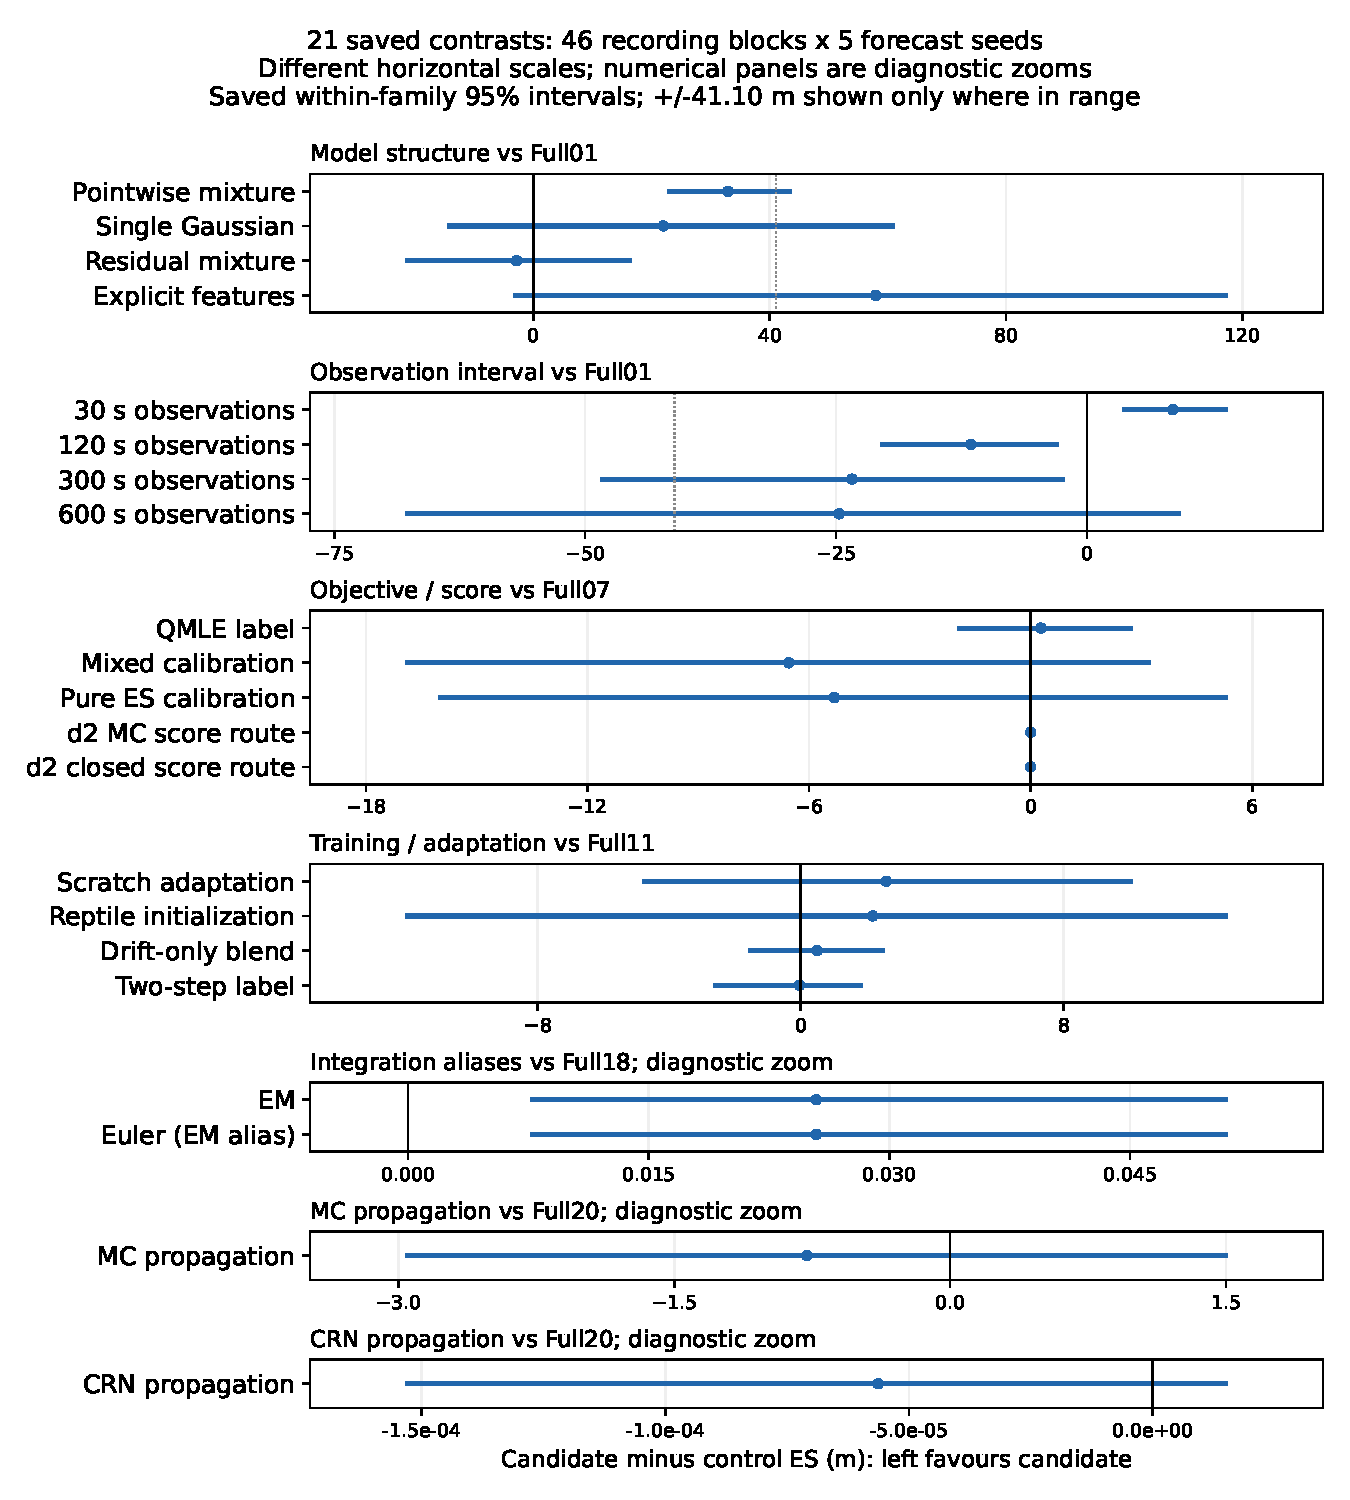
\includegraphics[height=.80\textheight,width=\linewidth,keepaspectratio]{../figures/preliminary-method-effects.pdf}
\caption{All 21 saved paired contrasts, with explicitly different horizontal
scales. Points are recording-block means of candidate-minus-control ES;
bars are saved within-family simultaneous 95\% intervals. Each panel names
its Full control; left of zero favours the candidate. Numerical panels are
diagnostic zooms, not enlarged practical effects. Dotted \(\pm41.10\)-m
boundaries appear only where within the axis range; they are outside the
smaller panels. Neither zoom nor crossing a line qualifies a conclusion.
The seven panels represent five method families: integration aliases, MC
propagation and CRN propagation are three axes of the numerical family.
Exact small differences and aliases remain in Table~\ref{tab:preliminary-method-effects}.}
\label{fig:preliminary-method-effects}\hypertarget{fig:preliminary-method-effects}{}
\end{figure}
\begin{figure}[p]
\centering
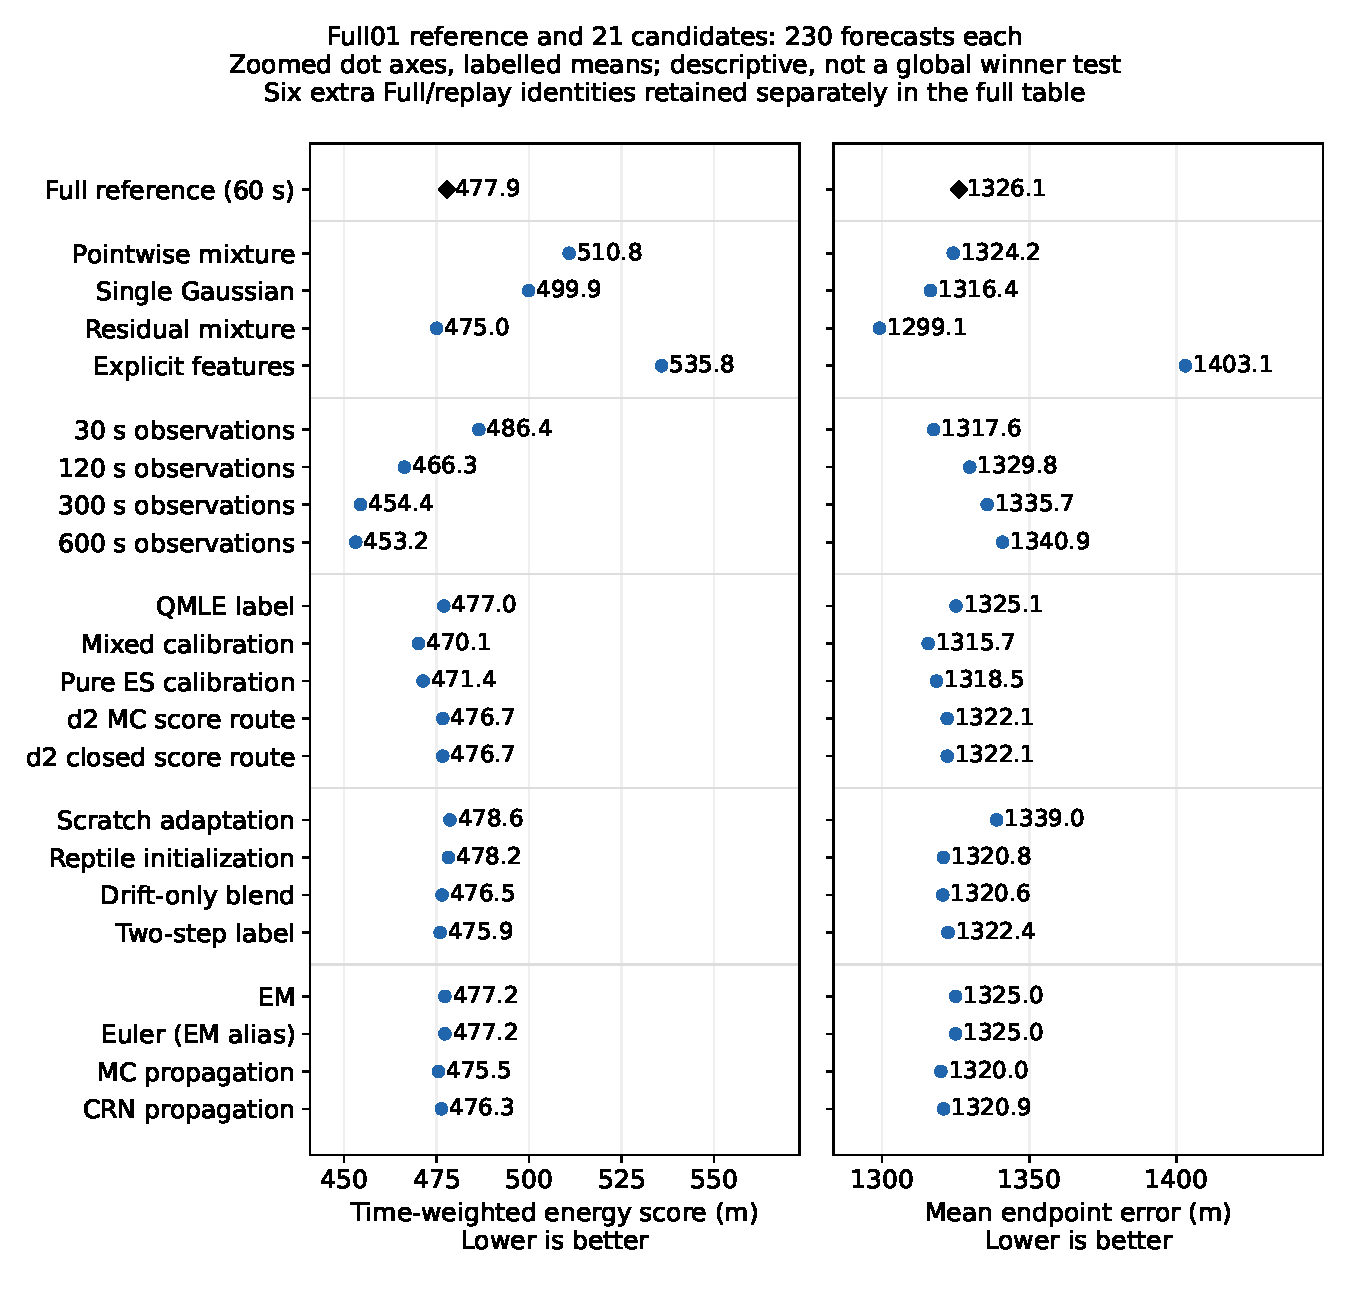
\includegraphics[height=.72\textheight,width=\linewidth,keepaspectratio]{../figures/preliminary-method-absolute.pdf}
\caption{Full01 reference and all 21 candidates, with numeric labels for
saved absolute ES and endpoint-error means in metres. Both dot axes are
zoomed and lower is better; differences in dot position are not paired
effect estimates. Observation variants follow increasing interval order.
Six extra Full/replay roles are omitted only from this display and are
retained separately, not averaged, in Table~\ref{tab:all-method-absolute}.
Each row uses all 230 predictions; scoring routes and aliases are not
independent algorithms. This is descriptive, not a global winner test.}
\label{fig:preliminary-method-absolute}\hypertarget{fig:preliminary-method-absolute}{}
\end{figure}

\FloatBarrier

\section{Horizon-dependent error and empirical coverage}
Full01's weighted ES is 477.85 m, whereas its mean 30-minute endpoint error
is 1326.09 m; these are different quantities.
The retained all-method aggregate reports marginal ES at each target, but
only the four-target average ADE and last-target FDE for point accuracy.
Those two summaries do not identify the earlier mean-position errors, and
ES cannot be converted into them. We do not reconstruct a complete point-error
profile from these summaries. The existing map cases separately retain
four-time mean-position errors, described in Section~\ref{sec:case-horizons};
they are terrain illustrations, not a substitute for all-method accuracy.
Table~\ref{tab:preliminary-coverage} shows increasing marginal ES and substantial
undercoverage of the nominal 90\% radial prediction disk at the longer times.
Coverage is averaged over five simulated ensembles for each of the same
46 targets, not over 230 independent observed targets. These proportions are
descriptive; no new coverage-test family or confidence interval is introduced.
The pattern does not identify a unique drift, diffusion or mixture failure.

\begin{table}[htbp]
\centering
\small
\caption{Descriptive saved-score horizon profile for the complete primary
Full01 grid; actual original target times follow the registered tolerance.}
\label{tab:preliminary-coverage}\hypertarget{tab:preliminary-coverage}{}
\begin{tabular}{@{}rrr@{}}
\toprule
Nominal horizon (min) & Full01 ES (m) & 90\% disk coverage (\%)\\
\midrule
1 & 50.57 & 95.65\\
5 & 243.23 & 37.83\\
15 & 609.27 & 35.22\\
30 & 1008.35 & 46.52\\
\bottomrule
\end{tabular}
\end{table}

\paragraph{The full configuration-by-horizon pattern.}
Figure~\ref{fig:all-method-horizons} extends the view to all 28 original
primary configurations, with full values in Table~\ref{tab:all-method-horizons}.
At the thirty-minute slot, their saved mean marginal ES spans 941.89--1197.62 m;
all nominal 90\% disk coverage means are below 90\%, ranging from
21.74\% to 79.13\%. These are ranges across configurations, not confidence
intervals, population bounds or a global best-model test.
The weighted primary summary can conceal a horizon-dependent tradeoff:
the residual mixture has lower ES than Full01 at five and fifteen minutes
(228.87 versus 243.23 m; 598.70 versus 609.27 m), but higher ES at thirty
minutes (1022.19 versus 1008.35 m). No per-horizon significance test is
introduced. The marginal ES is a distributional score, not mean position
error; higher coverage alone is not better calibration without considering
the nominal probability and region size.
These are original nominal target slots, not new interpolated exact-time
predictions. The \hyperref[sec:target-times]{saved target-clock description}
binds the three illustrated models,
not every prediction array of all 28 configurations. The separate completed
whole saved-output audit covers the complete score grid; neither this narrow
description nor that audit certifies a physically sourced target clock.
\begin{figure}[p]
\centering
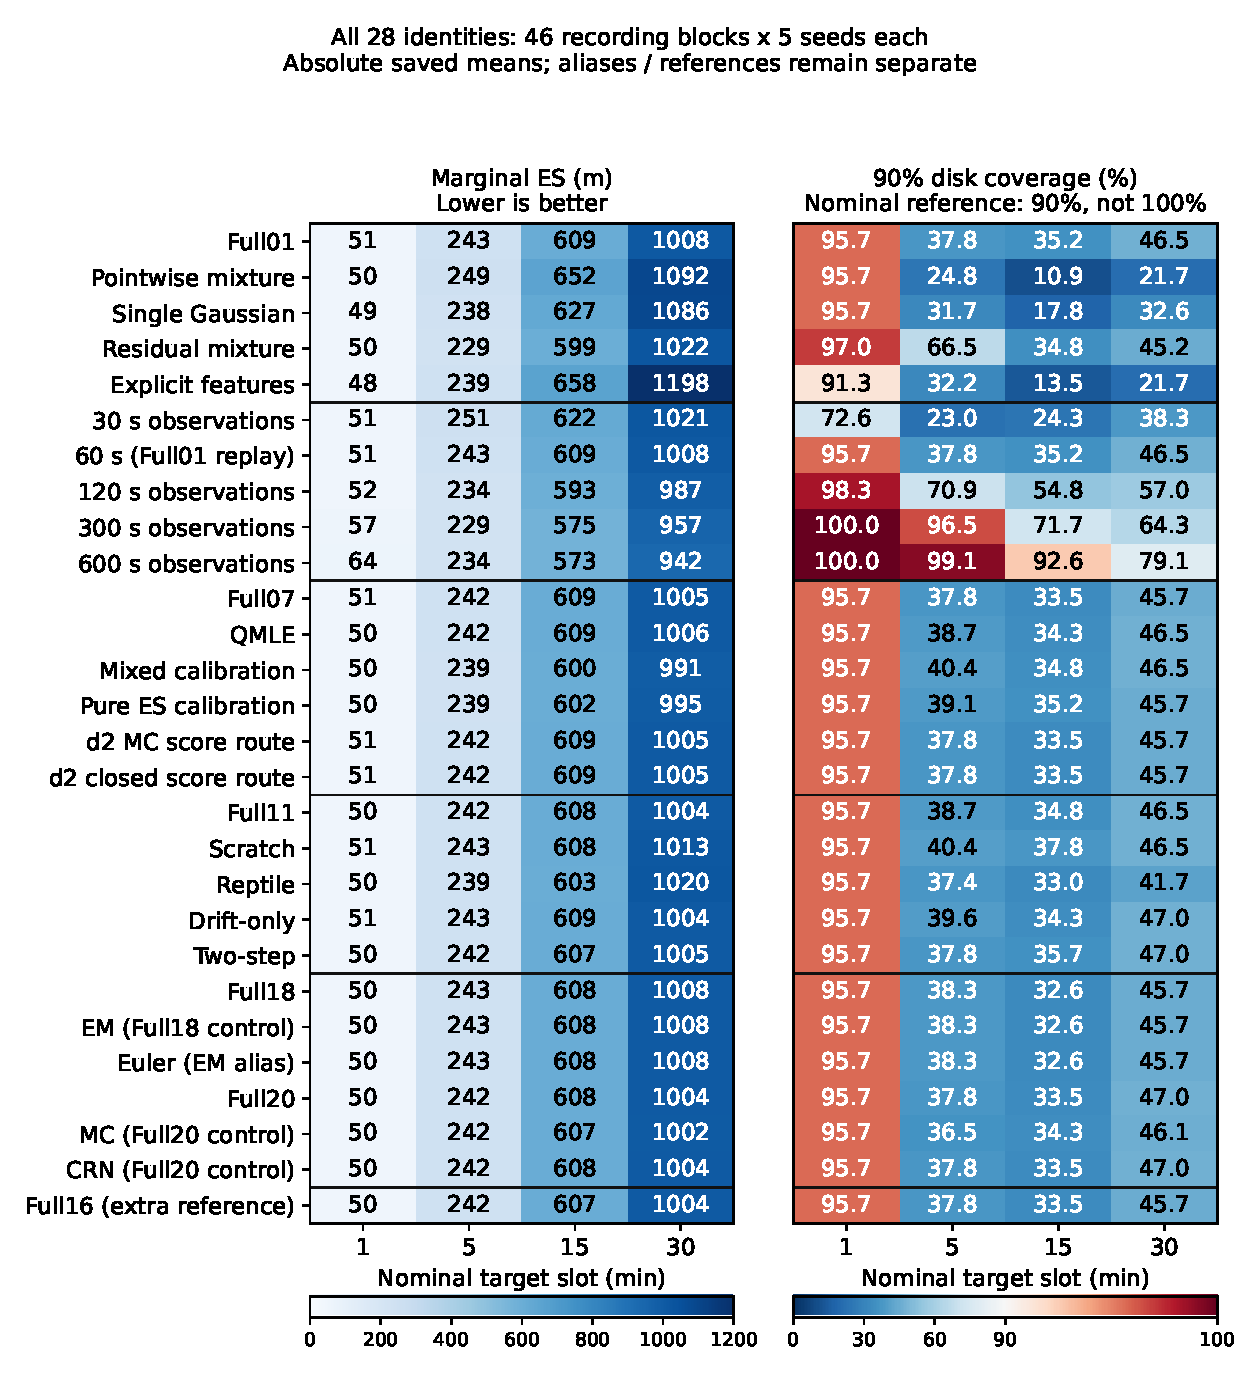
\includegraphics[height=.79\textheight,width=\linewidth,keepaspectratio]{../figures/revision46-corrections-v1/method-horizon-overview.pdf}
\caption{All 28 primary saved configurations at four nominal target slots; no intermediate-time prediction is added. Left: marginal ES (m), lower is better. Right: empirical nominal 90\% disk coverage (\%); 90\% is the calibration reference, not 100\%, and region sizes are not shown. Each cell averages the same 46 blocks and five seeds. ES is rounded to whole metres and coverage to one decimal for overview only; full-precision values and all roles remain in the saved projection and Table~\ref{tab:all-method-horizons}. Row order follows the declared families, not performance. Aliases and distinct Full controls are not pooled; similar rounded cells do not establish equivalence. Descriptive, not new per-horizon tests or final qualification.}
\label{fig:all-method-horizons}
\end{figure}


\FloatBarrier
\paragraph{Region size and coverage across all configurations.}
Figure~\ref{fig:all-method-regions} and Table~\ref{tab:all-method-regions}
extend the joint region description to every original primary configuration,
using the same 6440 saved scores, 46 blocks and five seeds. Each nominal
90\% disk cell reports mean area and target containment; the table also gives
mean radius. We average saved disk areas themselves, not the square of an
averaged radius. The full saved aggregate retains all four probability levels
at all four target slots. This extension reads saved score numbers only;
it does not rescore particles, interpolate targets or add predictions.

At thirty minutes, the 28 mean 90\% disk areas span 1.247--12.609 km\(^{2}\),
while empirical coverage spans 21.74--79.13\%, always below nominal 90\%.
dt600 has the largest area and highest observed coverage in this finite
display: 12.609 km\(^{2}\) and 79.13\%, versus Full01's 4.534 km\(^{2}\)
and 46.52\%. Its area is about 2.78 times Full01's, yet its mean endpoint
error is slightly higher (1340.94 versus 1326.09 m). Thus its higher coverage
does not simultaneously establish sharper regions, better point accuracy
and calibration. dt600 changes fitted observation spacing, historical inputs
and noise estimation, not only the prediction integration step; these
descriptive comparisons do not identify which change produces the pattern.

Nor is the area--coverage relation uniform across horizons. At five minutes,
the residual mixture has a larger mean area than Full01 (0.400 versus
0.294 km\(^{2}\)) and higher coverage (66.52\% versus 37.83\%); at thirty
minutes its area is smaller (3.079 versus 4.534 km\(^{2}\)) and coverage
is slightly lower (45.22\% versus 46.52\%). The display therefore reveals
horizon-dependent descriptive tradeoffs, not a universal size--quality rule,
global winner test or causal mechanism. No new per-horizon interval or
calibration adjustment is introduced; block-resolved diagnostics remain
the three-model description below. The completed independent output replay
does not turn those three illustrative models into all-configuration
block-resolved calibration evidence.
\begin{figure}[p]
\centering
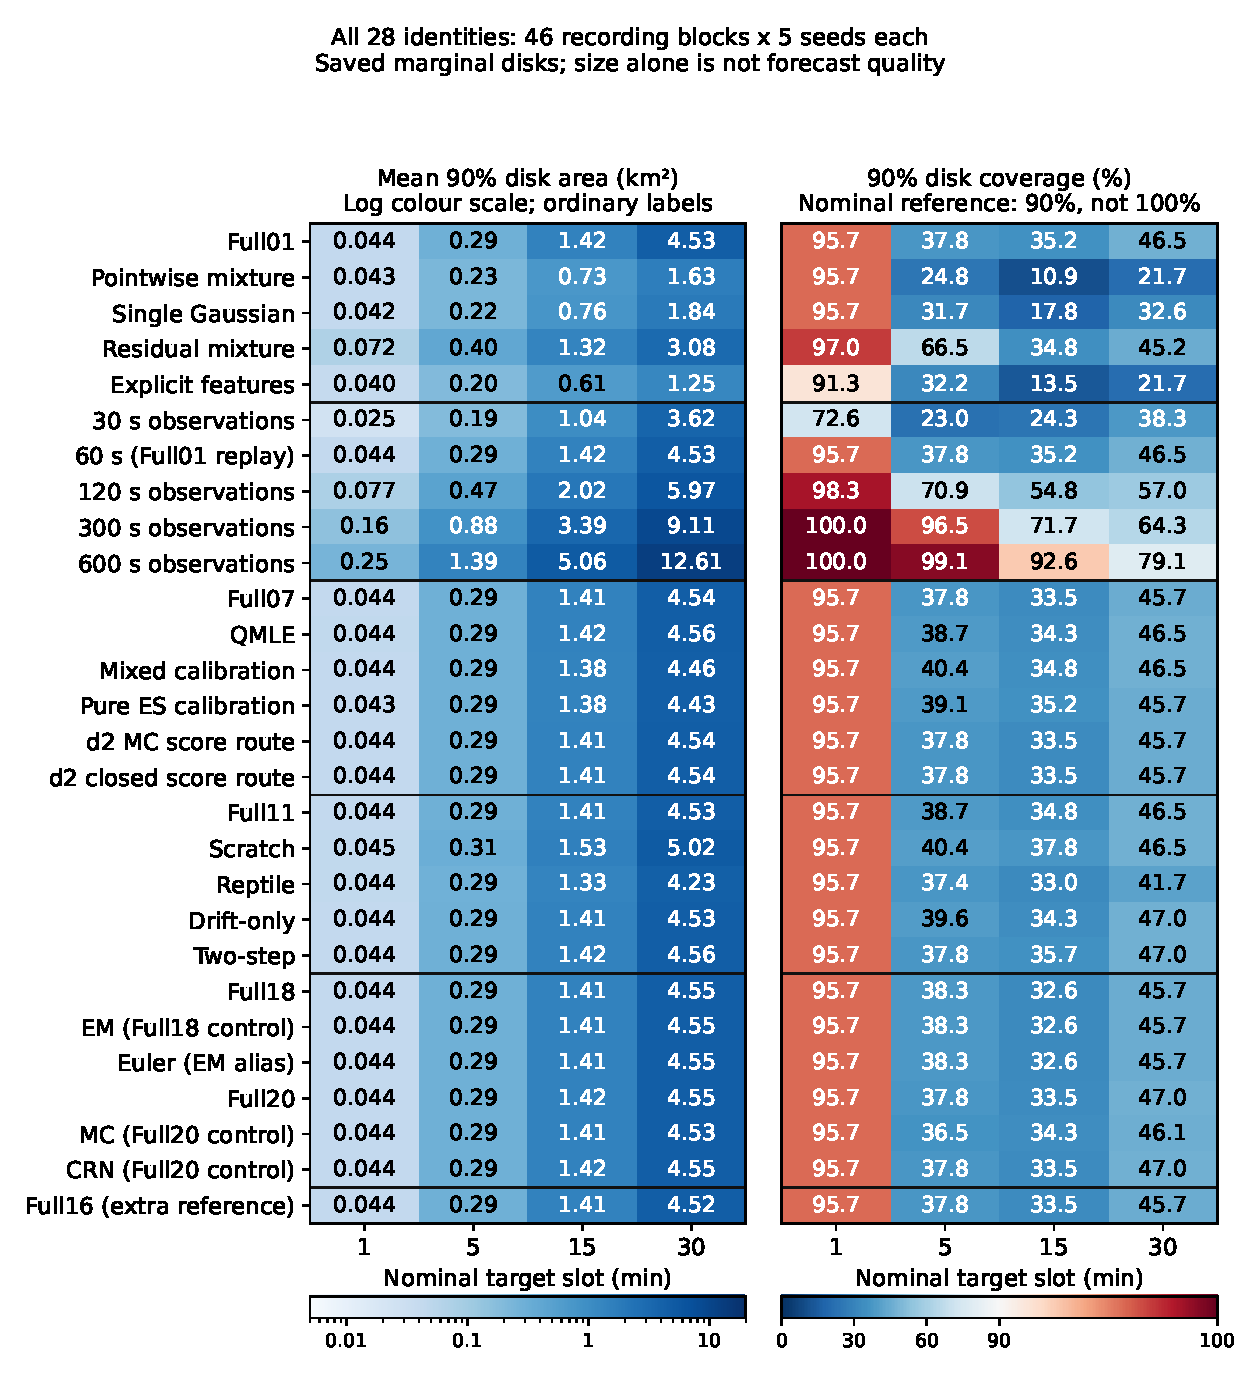
\includegraphics[height=.76\textheight,width=\linewidth,keepaspectratio]{../figures/revision46-corrections-v1/method-region-overview.pdf}
\caption{Complete 28-configuration region-size and coverage display at four original target slots. Left: mean nominal 90\% disk area (km$^2$); colour uses a logarithmic scale to show both short- and long-horizon areas, while cell labels give ordinary areas. Right: empirical target containment (\%), whose nominal reference is 90\%, not 100\%. Neither area nor coverage is a stand-alone quality ranking. Row order follows the declared method families, not observed performance; aliases and Full controls remain distinct. Each cell averages five seeds within each of 46 blocks and then equally over blocks. Descriptive means without new tests, prediction or recalibration; radii and exact values appear in Table~\ref{tab:all-method-regions} and the saved aggregate.}
\label{fig:all-method-regions}
\end{figure}

\FloatBarrier

\paragraph{All probability levels and the cost of wider regions.}
The complete 28-configuration profiles also show that the coverage mismatch
depends on nominal probability, not only horizon
(Table~\ref{tab:all-level-coverage}). At one minute, 24 configurations have
50\% disk coverage below 50\%, whereas 27 have 90\% disk coverage above
90\%. Thus high short-horizon coverage at one probability level does not
establish calibration of the predictive distribution. At thirty minutes,
all 28 are below nominal at the 80\%, 90\% and 95\% levels; observed
95\% coverage spans 26.52--87.39\%. At the 50\% level, 27 are below
nominal and one equals it, without certifying that configuration's other
levels. These are counts and ranges of saved configuration means, not
independent algorithm replications or confidence intervals: aliases and
Full controls remain in the frozen inventory. The table reports area
ranges alongside coverage; widening the same predictor's disk can raise
containment without repairing its mean-position error. No probability
level is changed, and no new calibration test or fitted correction is made.

We additionally describe the same 690 previously displayed primary scores
for Full, GMM kernel and dt300, with no new forecasts, particle rescoring or
inference tests. Each original score stores all four marginal disk levels.
Table~\ref{tab:full-calibration-area} reports Full's coverage and mean disk
area together. Mean area averages \(\pi r_{p,t}^2\) over seeds within each
block and then equally over 46 blocks; it is not
\(\pi\{\operatorname{mean}(r_{p,t})\}^2\).

\begin{table}[htbp]
\centering\small
\caption{Full's complete primary saved-region profile. Each cell is
observed coverage (\%) / mean disk area (km\(^{2}\)); column headings
are nominal probabilities, not observed coverage.}
\label{tab:full-calibration-area}\hypertarget{tab:full-calibration-area}{}
\begin{tabular}{rrrrr}
\toprule
Horizon (min) & 50\% & 80\% & 90\% & 95\%\\
\midrule
1 & 33.04 / 0.013 & 87.39 / 0.031 & 95.65 / 0.044 & 96.52 / 0.057\\
5 & 6.52 / 0.094 & 25.65 / 0.210 & 37.83 / 0.294 & 50.43 / 0.378\\
15 & 9.57 / 0.539 & 24.35 / 1.062 & 35.22 / 1.415 & 43.91 / 1.753\\
30 & 33.48 / 2.002 & 37.39 / 3.552 & 46.52 / 4.534 & 52.17 / 5.496\\
\bottomrule
\end{tabular}
\end{table}

The long-horizon mismatch persists beyond the 90\% level: at thirty minutes,
Full's nominal 95\% disk covers only 52.17\% of targets on average over
ensembles. At one minute, nominal 50\% and 90\% disks cover 33.04\% and
95.65\%, respectively, showing that the mismatch depends on probability
level as well as horizon. These are descriptive measurements, not new
significance statements or proof of a particular failure mechanism.

\begin{table}[htbp]
\centering\small
\caption{Thirty-minute nominal 90\% disk profiles on the same original
46 blocks and five ensembles per model. A smaller area is not preferable
without adequate coverage; larger coverage alone need not imply calibration.}
\label{tab:model-region-size}\hypertarget{tab:model-region-size}{}
\begin{tabular}{lrrr}
\toprule
Model & Coverage (\%) & Mean area (km\(^{2}\)) & Mean radius (m)\\
\midrule
Full & 46.52 & 4.534 & 1183.6\\
GMM kernel & 45.22 & 3.079 & 989.5\\
dt300 & 64.35 & 9.109 & 1692.8\\
\bottomrule
\end{tabular}
\end{table}

The dt300 disk has higher thirty-minute coverage than Full, but its mean
area is about twice as large and its coverage remains well below nominal
90\%. Its mean endpoint error is also slightly higher (1335.73 versus
1326.09 m). Thus improved ES or increased coverage cannot be interpreted as
a sharper, more accurate and calibrated forecast simultaneously. GMM's
smaller thirty-minute region similarly does not establish better precision
when coverage remains low. This three-model display is post-outcome
descriptive reporting of already selected examples, not a global ranking,
an additional hypothesis family or a model-selection rule.
The projection \path{paper/pirc17/calibration-description-v1.json} retains
the complete original 690-score bindings without private trajectory IDs
or coordinates. Its ES, FDE and 90\% coverage reconcile to the unchanged
original stage table. Missing, failed, duplicate or wrong-source rows reject
the whole projection. The separate independent saved-output audit is complete;
this descriptive projection does not itself establish calibration or participant
independence.

\begin{figure}[htbp]
\centering
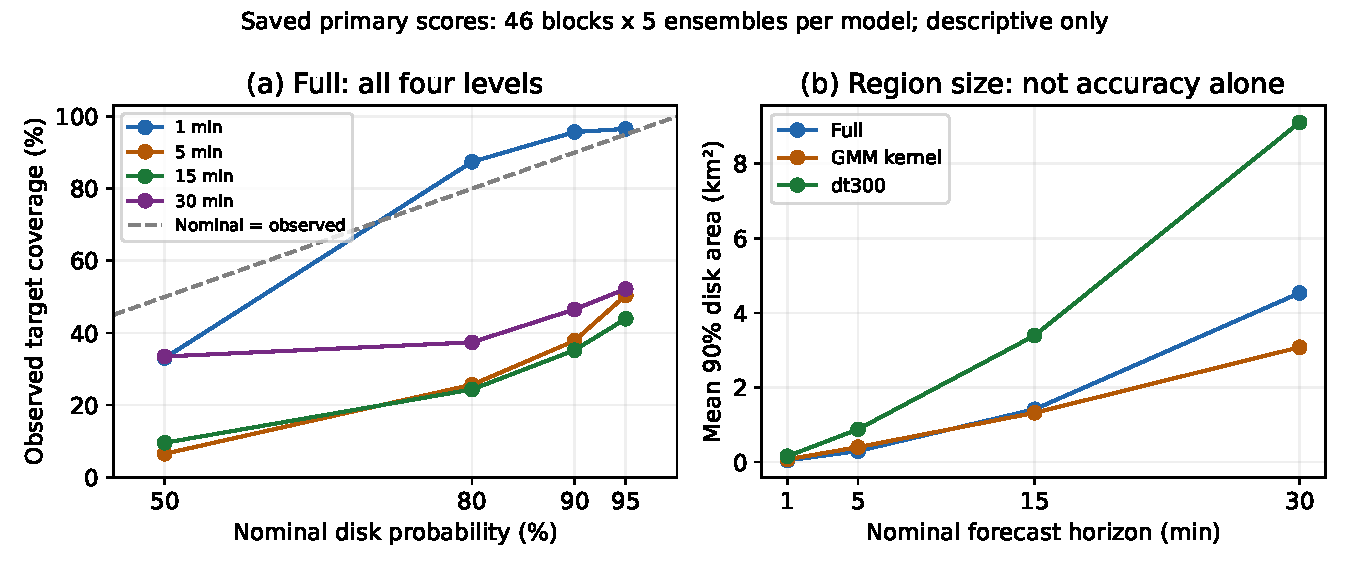
\includegraphics[width=\linewidth]{../figures/preliminary-calibration-area.pdf}
\caption{Saved calibration and region-size diagnostics, not new experiments.
Left: Full's observed coverage against nominal probability, separately for
each horizon; the diagonal denotes nominal agreement. Right: mean 90\% disk
area for the three previously displayed models. Connecting lines only guide
the eye between four measured levels or horizons; there is no intermediate
target evaluation, simultaneous path coverage, or new statistical test.}
\label{fig:calibration-area}\hypertarget{fig:calibration-area}{}
\end{figure}

\paragraph{Variation across recording blocks.}\label{sec:block-calibration}\hypertarget{sec:block-calibration}{}
For a fixed model, target slot and disk probability level, we first average
the five forecast seeds within each of the same 46 recording blocks:
\begin{equation}
 C_b=\frac{1}{5}\sum_s\mathbf{1}\{y_b\in D_{bs}\},\qquad
 a_b=\frac{1}{5}\sum_s\frac{|D_{bs}|}{10^6}.
 \label{eq:block-calibration-summary}\hypertarget{eq:block-calibration-summary}{}
\end{equation}
Here \(D_{bs}\) is the saved marginal disk, \(C_b\) is a descriptive
containment fraction and \(a_b\) is mean area in square kilometres.
Five seeds repeat prediction of the same real target; they are not five
independent observations. Individual \(C_b\) values lie on a 0.2 grid.
Table~\ref{tab:block-calibration} reports medians and interquartile ranges
over blocks; linear-interpolated quantiles at \((46-1)p\) need not lie on
that grid and are not confidence intervals. All four saved levels and
horizons are retained in \path{paper/pirc17/calibration-block-description-v1.json};
the table and Figure~\ref{fig:block-calibration} show nominal 90\% disks only.

\begin{table}[htbp]
\centering\small
\caption{Original 46-block distributions of nominal 90\% disks.
Coverage and area are median [25th, 75th percentile]; the last columns
count blocks with zero/all five seeds covering their target.}
\label{tab:block-calibration}\hypertarget{tab:block-calibration}{}
\begin{tabular}{@{}lrl lrr@{}}
\toprule
Model & Min & Coverage (\%) & Area (km$^2$) & 0/5 & 5/5\\
\midrule
Full & 1 & 100 [100, 100] & 0.043 [0.042, 0.046] & 2 & 44\\
Full & 5 & 0 [0, 100] & 0.280 [0.261, 0.308] & 26 & 16\\
Full & 15 & 0 [0, 100] & 1.285 [1.150, 1.557] & 29 & 15\\
Full & 30 & 10 [0, 100] & 4.022 [3.405, 4.966] & 23 & 20\\
\midrule
GMM kernel & 1 & 100 [100, 100] & 0.072 [0.070, 0.074] & 1 & 44\\
GMM kernel & 5 & 100 [5, 100] & 0.401 [0.389, 0.411] & 12 & 28\\
GMM kernel & 15 & 0 [0, 100] & 1.322 [1.300, 1.357] & 28 & 14\\
GMM kernel & 30 & 0 [0, 100] & 3.088 [3.000, 3.179] & 24 & 20\\
\midrule
dt300 & 1 & 100 [100, 100] & 0.155 [0.150, 0.159] & 0 & 46\\
dt300 & 5 & 100 [100, 100] & 0.871 [0.832, 0.894] & 1 & 44\\
dt300 & 15 & 100 [20, 100] & 3.264 [3.060, 3.497] & 11 & 31\\
dt300 & 30 & 100 [0, 100] & 8.518 [7.707, 9.564] & 16 & 29\\
\bottomrule
\end{tabular}
\end{table}

At 30 minutes Full has 23 of 46 blocks with no covered seed and 20 with
all five covered, despite overall coverage of 46.52\%. Its area median is
4.022 km$^2$ [3.405, 4.966], with range 2.963--11.551 km$^2$.
The dt300 median containment is 100\%, but 16 blocks still have zero
covered seeds; its area median is 8.518 km$^2$ [7.707, 9.564].
Neither an overall mean nor a high median establishes reliable
conditional calibration, deployment readiness or which component causes
the observed misses.

For a coordinate-free example, anonymous block B13 is the first saved
block in the original ordering with Full 0/5 and dt300 5/5 containment
at 30 minutes. Full, GMM and dt300 have 0/5, 0/5 and 5/5 containment
and mean areas 3.489, 3.204 and 8.260 km$^2$, respectively. This example
is selected after seeing outcomes to illustrate size/containment, not
to infer superiority. No route or geographic identity is released;
the separate permissions for real map cases remain unverified.

\begin{figure}[p]
\centering
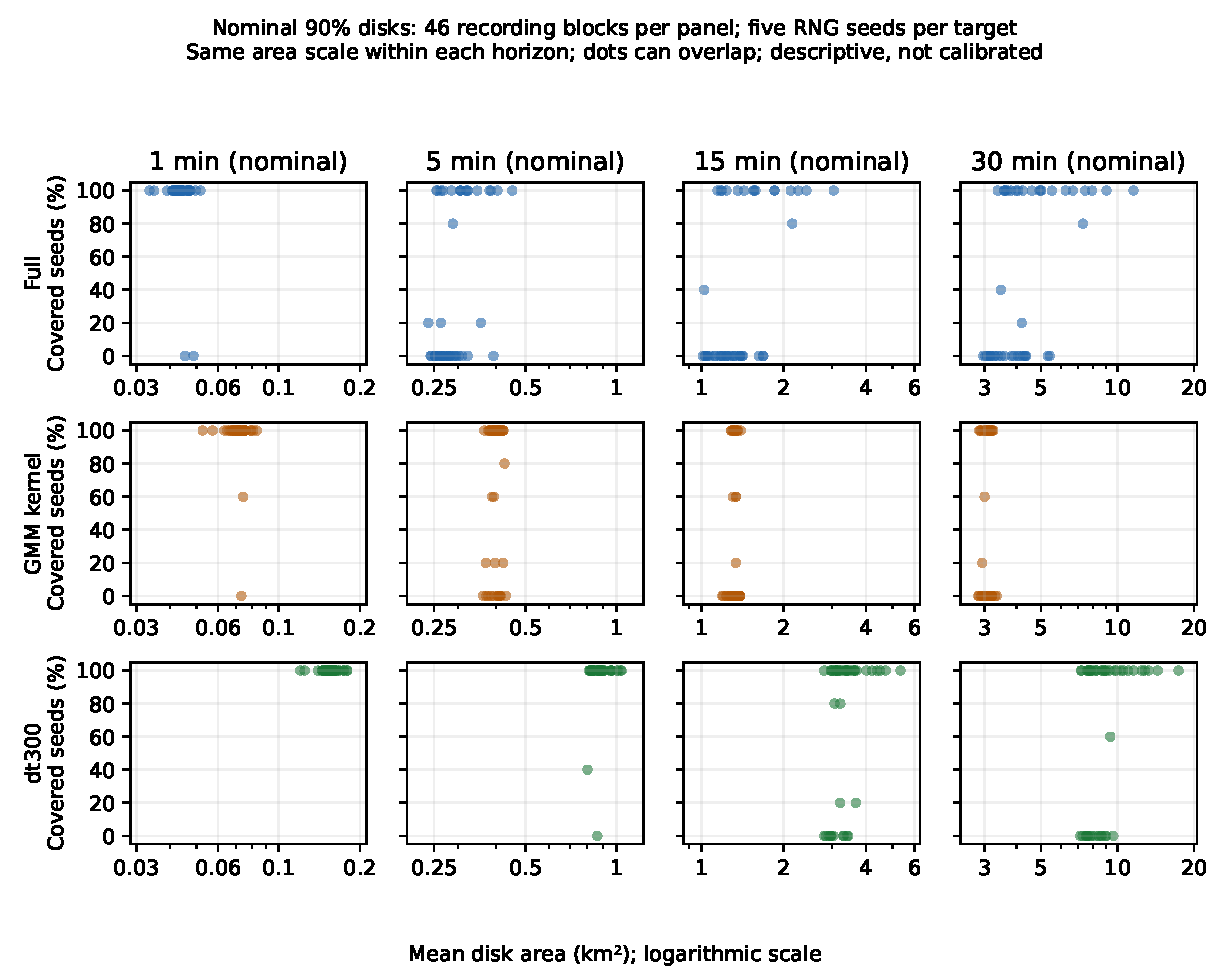
\includegraphics[width=\linewidth]{../figures/preliminary-calibration-blocks.pdf}
\caption{Paired block-level size and containment for the three previously
displayed models at four nominal horizons. Each point is one recording
block averaged over five forecast seeds; points can overlap. Area uses
a logarithmic scale, shared across models within each horizon, while
containment is the fraction of five saved disks containing the same
target. These are not 46 estimates of population calibration; no
simultaneous path coverage, new hypothesis test or post-hoc radius
rescaling is performed.}
\label{fig:block-calibration}\hypertarget{fig:block-calibration}{}
\end{figure}

The known-velocity structure and observation-interval families each contain
one failed required row and remain unavailable as complete families. The
other complete six-block secondary summaries are descriptive only.
Missing rows and failed comparisons are not filled with zero, deleted to
form a favourable successful intersection, or replaced by primary-mode data.

\begin{figure}[htbp]
\centering
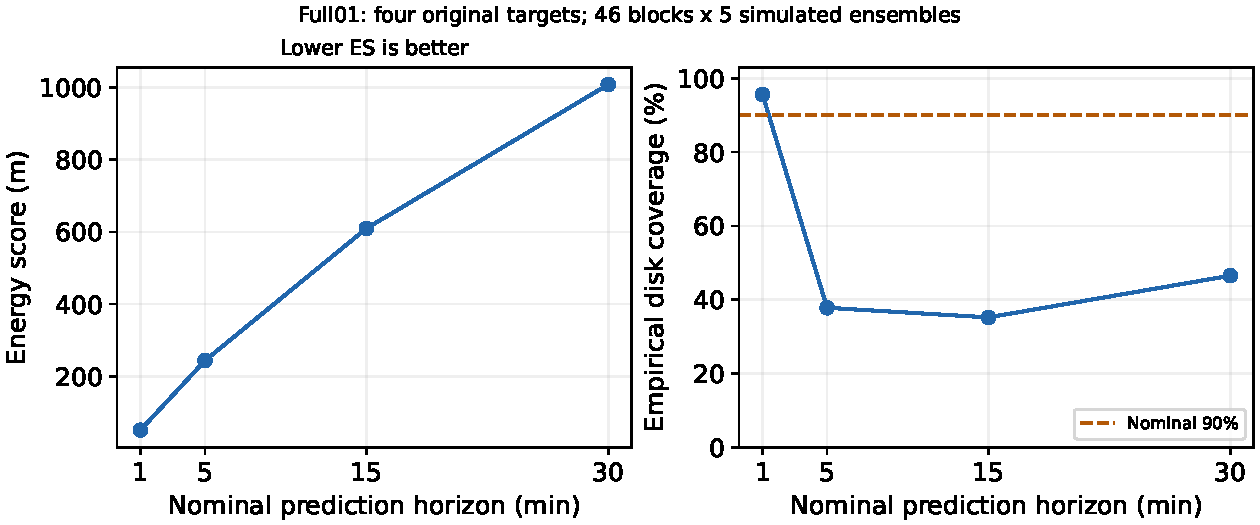
\includegraphics[width=\linewidth]{../figures/revision46-corrections-v1/preliminary-full-horizons.pdf}
\caption{Full01's actual aggregate saved scores and coverage at the four
original targets. The dashed line is nominal 90\% coverage; observed
30-minute coverage is only 46.52\%. Lines guide the eye, not intermediate
observations or a survival curve. These are distribution-level summaries,
not trajectory/map overlays or independent 230-target measurements.}
\label{fig:preliminary-full-horizons}\hypertarget{fig:preliminary-full-horizons}{}
\end{figure}


\section{Descriptive method results by origin cover}
\label{sec:origin-cover-results}\hypertarget{sec:origin-cover-results}{}
To make environmental coverage visible, Table~\ref{tab:origin-cover-methods}
describes Full, GMM and dt300 using all 690 existing scores from their
original $3\times46\times5$ primary grid. Within each block, five simulation
seeds are averaged first; block means are then averaged within the original
WorldCover origin category. ES still averages the four registered target
times, while FDE measures the last target. The category-weighted totals
reconcile to the unchanged primary method table. Missing, failed, duplicate
or wrong-source rows reject the whole descriptive projection; no
successful-subset summary is substituted.

\begin{table}[htbp]
\centering\small
\caption{Descriptive origin-category means, ES/FDE in metres. No subgroup
confidence intervals, hypothesis tests or environmental-effect verdicts.}
\label{tab:origin-cover-methods}\hypertarget{tab:origin-cover-methods}{}
\begin{tabular}{lrrrr}
\toprule
Origin pixel & Blocks & Full & GMM & dt300\\
\midrule
Trees & 27 & 427.66/1184.64 & 420.85/1153.52 & 414.59/1203.95\\
Grass & 9 & 556.86/1597.16 & 557.16/1587.72 & 514.09/1579.13\\
Cropland & 3 & 623.14/1678.49 & 589.40/1591.57 & 600.89/1775.32\\
Built-up & 7 & 507.60/1372.16 & 529.38/1364.23 & 468.75/1342.70\\
\bottomrule
\end{tabular}
\end{table}

These are post-outcome descriptions, not preregistered subgroup inference.
For example, dt300 has a lower mean ES but a higher FDE in the tree and
cropland origin categories; GMM has a higher ES but a slightly lower FDE in
the built-up category. These patterns illustrate different metric rankings,
not causal terrain effects or robust category-specific model superiority.
The cropland group contains only three recording-hash blocks, not 15
independent trajectories. The seven absent origin classes retain null
metrics in the projection. Formal method inference remains on all 46
blocks; actual terrain effects require the separate registered terrain
comparisons and their evidence qualification.

\FloatBarrier
\subsection{A completed constant-velocity reference}
\label{sec:inertial-primary}
The registered inertial reference extrapolates the saved causal initial velocity: $\widehat x^{\mathrm{I}}(t)=x_0+t\widehat v_0$. It is a deterministic path, not a fitted SDE or five repeated particle forecasts. All 58 registered reference paths have saved scores; Tables~\ref{tab:inertial-primary} and~\ref{tab:inertial-horizons} use the entire prespecified 46-block primary population, not the 12 secondary origins. Each reference is paired with Full at the same origin, target identity and actual target times. Average the five Full forecast seeds within each block first, then weight all 46 recording-hash blocks equally; the reference is never counted five times.

\begin{table}[htbp]\centering\small
\caption{Same primary origins and saved target slots. All errors are in metres and lower is better. ES evaluates the predictive distribution; ADE/FDE evaluate its mean path. Inertial is a point mass, so its ES equals displacement error. Counts are saved forecasts, not independent people or fitted models. Descriptive means only; no new confidence interval, significance test or qualification.}\label{tab:inertial-primary}
\begin{tabular}{@{}lrrrrr@{}}\toprule
Model & Forecasts & Blocks & Weighted ES & ADE & FDE\\\midrule
Inertial & 46 & 46 & 824.73 & 824.73 & 2095.78\\
Full & 230 & 46 & 477.85 & 636.11 & 1326.09\\
\bottomrule\end{tabular}\end{table}

\begin{table}[htbp]\centering\small
\caption{Mean marginal ES in metres at the four nominal target slots; lower is better. Actual retained-clock targets are 49--67, 294--305, 889--910 and 1785--1814 seconds under the unchanged original 30-second tolerance. Neither target interpolation nor a new simulation is used.}\label{tab:inertial-horizons}
\begin{tabular}{@{}lrrrr@{}}\toprule
Model & 1 min & 5 min & 15 min & 30 min\\\midrule
Inertial & 31.17 & 237.93 & 934.03 & 2095.78\\
Full & 50.57 & 243.23 & 609.27 & 1008.35\\
\bottomrule\end{tabular}\end{table}

Full-minus-inertial mean differences are -346.87 m for weighted ES, -188.62 m for ADE and -769.69 m for FDE. Full has strictly lower weighted ES in 34 of 46 blocks. However, the inertial reference has lower mean ES at 1 and 5 minutes, whereas Full has lower mean ES at 15 and 30 minutes. Thus the aggregate benefit is not uniform across horizons.

These are post-outcome descriptive comparisons of existing scores, not a registered component contrast or an independently audited superiority claim. No inference is made from the 34/46 count; recording hashes do not certify independent participants. The original validation-based $\delta=41.100259$ m is not recalibrated from this final-evaluation reference. Original output verification, final cards and human review remain pending; no superiority over the cited external models or deployment calibration follows.
\FloatBarrier

\FloatBarrier
\subsection{Point error at each saved target time}
\label{sec:point-error-horizons}
ES evaluates an entire predictive distribution and is not the distance between its mean and the observed position. Table~\ref{tab:point-error-horizons} makes that distance explicit for the already-described Full/GMM/dt300 comparison and the inertial reference; it is not a new ranking of all 28 configurations. Use the original saved scoring-disk center $c_{m,b,s,k}$ (the 512-particle mean, or the deterministic reference position) and the same saved target $y_{b,k}$ in the same origin-local scoring frame. No forecast arrays, new particle scores, target interpolation or simulation are needed.

For model $m$, average errors over its $S_m$ original seeds within each recording-hash block, then equal-weight all 46 blocks. Here $S_m=5$ for the three probabilistic configurations and $S_m=1$ for the reference; a reference is not counted five times:
\begin{equation}
\bar e_{m,k}=\frac{1}{46}\sum_{b=1}^{46}
\frac{1}{S_m}\sum_{s=1}^{S_m}\lVert c_{m,b,s,k}-y_{b,k}\rVert_2.
\label{eq:point-error-horizon-mean}
\end{equation}

\begin{table}[htbp]\centering\small
\caption{Mean saved-center displacement error in metres; lower is better. The four columns use the original nominal 1/5/15/30-minute target slots, with actual retained-clock ranges 49--67, 294--305, 889--910 and 1785--1814 s and unchanged 30-second tolerance. Rows are saved forecasts, not independent targets or people. Descriptive values only; no per-horizon inference.}\label{tab:point-error-horizons}
\begin{tabular}{@{}lrrrrr@{}}\toprule
Model & Rows & 1 min & 5 min & 15 min & 30 min\\\midrule
Full & 230 & 73.77 & 332.31 & 812.26 & 1326.09\\
GMM & 230 & 71.92 & 323.79 & 792.99 & 1299.11\\
dt300 & 230 & 75.88 & 340.10 & 825.76 & 1335.73\\
Inertial & 46 & 31.17 & 237.93 & 934.03 & 2095.78\\
\bottomrule\end{tabular}\end{table}

All 736 selected saved rows match the same 184 target positions. For every row, the arithmetic mean of these four errors and its last error reproduce the original saved ADE and FDE within floating-point roundoff; the maximum discrepancy is below $10^{-12}$ m. Averaging at each target before taking the Euclidean norm would be a different estimator and is not used.

The inertial reference has lower mean point error at 1 and 5 minutes; Full has lower mean point error at 15 and 30 minutes. GMM has slightly lower descriptive mean errors than Full at all four slots. Conversely, dt300 has larger mean-position errors than Full at every slot despite its lower saved aggregate ES. Thus a distribution-score improvement is not automatically an improvement in mean-path location. Here dt300 denotes the training observation interval, not the integration step. No statistical superiority, independent-participant generalization or deployment accuracy follows from these post-outcome means; original final inference, output audit and review remain pending.
\FloatBarrier



\section{Marginal CRPS and within-forecast endpoint error quantiles}
\label{sec:secondary-score-diagnostics}\hypertarget{sec:secondary-score-diagnostics}{}
Table~\ref{tab:crps-endpoint-diagnostics} uses the same four models already
compared above, not a new selection by the best diagnostic value. Coordinate
CRPS measures the local east/north marginal distributions in metres; lower is
better on that marginal, but two good marginals do not certify the joint
distribution, dependence structure or predictive-disk calibration. The two
coordinate scores are not summed and renamed joint ES.

The lower panel distinguishes mean-position FDE from particle endpoint-error
quantiles. For each original forecast, the stored $q_{.50}$, $q_{.90}$ and
$q_{.95}$ are quantiles of particle distances to that forecast's observed
endpoint. We average those already-saved quantiles over seeds and recording
blocks. They are neither population FDE quantiles nor quantiles after pooling
particles across cases, and are not radii around the ensemble mean. No best
particle is selected. Inertial is a single point, so all three per-forecast
quantiles equal its FDE before aggregation.

The diagnostics show why one score cannot stand for all prediction quality.
At nominal 30 minutes, dt300 has lower east/north CRPS than Full01
(687.11/524.07 versus 737.72/535.72 m), yet a slightly higher mean-position
FDE (1335.73 versus 1326.09 m) and a larger mean within-forecast $q_{.95}$
(2827.57 versus 2346.62 m). GMM's corresponding $q_{.95}$ is 2138.12 m,
not a promise that a 2138.12 m predictive disk has 95\% target coverage.
These means are descriptive; no per-horizon significance, general superiority
or causal explanation is added, and the reported long-horizon undercoverage
remains a limitation.

The complete \path{paper/pirc17/secondary-scores-v1/} supplement retains all
120 configuration/mode views and 480 repeated time views from the original
11368 score rows, including five configuration/mode views with failed required
rows and null means. Seeds are averaged within origins and then equally
across the same recording-hash blocks; inertial is not repeated five times.
No prediction, particle scoring or resampling is repeated. The anonymous
projection binds source export \texttt{29cb892f}, audit \texttt{8ff917ad} and
analysis \texttt{d1d67a3b}; actual recorded target-time ranges are retained,
without certifying physical UTC or independent participants.
\begin{table}[htbp]
\centering\small
\caption{Saved marginal CRPS and within-forecast endpoint error quantiles (metres). Lower CRPS is better for that coordinate; two marginals do not determine joint calibration. Each stochastic configuration uses 46 recording-hash blocks and five seeds (230 forecasts); inertial uses the same 46 blocks with one deterministic path each. Quantile entries are block/seed means of per-forecast particle error quantiles, not population FDE quantiles, pooled particles or a best-particle path. All targets retain their original recorded elapsed time; no per-horizon hypothesis test.}
\label{tab:crps-endpoint-diagnostics}
\begin{tabular}{@{}lrrr@{}}
\toprule
Model & Nominal min & CRPS east & CRPS north\\
\midrule
Full01 & 1 & 32.71 & 31.55\\
Full01 & 5 & 157.30 & 153.31\\
Full01 & 15 & 390.26 & 373.30\\
Full01 & 30 & 737.72 & 535.72\\
GMM & 1 & 32.58 & 31.51\\
GMM & 5 & 149.27 & 142.28\\
GMM & 15 & 384.50 & 367.09\\
GMM & 30 & 736.79 & 549.33\\
dt300 & 1 & 37.20 & 34.78\\
dt300 & 5 & 147.70 & 144.49\\
dt300 & 15 & 368.85 & 354.71\\
dt300 & 30 & 687.11 & 524.07\\
Inertial & 1 & 21.37 & 18.50\\
Inertial & 5 & 137.90 & 160.72\\
Inertial & 15 & 561.23 & 618.27\\
Inertial & 30 & 1297.37 & 1356.32\\
\bottomrule
\end{tabular}
\par\medskip
\begin{tabular}{@{}lrrrr@{}}
\toprule
Model & Mean FDE & Mean $q_{.50}$ & Mean $q_{.90}$ & Mean $q_{.95}$\\
\midrule
Full01 & 1326.09 & 1564.98 & 2205.44 & 2346.62\\
GMM & 1299.11 & 1419.34 & 1979.14 & 2138.12\\
dt300 & 1335.73 & 1663.28 & 2585.48 & 2827.57\\
Inertial & 2095.78 & 2095.78 & 2095.78 & 2095.78\\
\bottomrule
\end{tabular}
\end{table}



\section{Local route illustrations withheld from public review}
\label{sec:case-horizons}\hypertarget{sec:case-horizons}{}
The owner's local manuscript retains three real-map cases at nominal
1, 5, 15 and 30 minutes. This public review projection intentionally
withholds their route maps and case-level diagnostics pending privacy and
map-publication permission. No missing illustration is replaced with
synthetic data, and no new forecast is generated. The original complete
local version is a separate review artifact; this projection does not
validate the withheld evidence or establish population terrain effects.

\clearpage

\section{Construction of the saved population descriptions}
\label{sec:population-description-construction}\hypertarget{sec:population-description-construction}{}
The duration, speed and source-label tables describe the original candidate
population, not a new eligibility screen. Their construction records are
collected here so that the main text can focus on the restricted evaluation
population and its scientific limitations.

\paragraph{Follow-up support before and after selection.}\label{sec:final-cohort-durations}\hypertarget{sec:final-cohort-durations}{}
Table~\ref{tab:final-cohort-durations} describes the same complete candidate
population, not only successful forecasts. Follow-up is
$D=t_{\mathrm{last}}-t_{\mathrm{origin}}$ for each original window.
All 12,370 windows retain their original qualification and selection;
invalid clock windows are neither dropped nor clipped. Equal-window
descriptions do not make multiple windows of a recording independent participants.

\begin{table}[htbp]
\centering\small
\caption{Recorded origin-to-last-observation follow-up spans (seconds). The first row is the denominator; the remaining four rows partition all windows. Brackets show interquartile ranges, not confidence intervals. Each original window contributes once.}
\label{tab:final-cohort-durations}\hypertarget{tab:final-cohort-durations}{}
\begin{tabular}{@{}lrrrr@{}}
\toprule
Window group & Count & Median [Q25,Q75] & Min--max & $\geq1800$s\\
\midrule
Released & 12,370 & 69.8 [30,203] & 2--4183 & 130\\
Temporal exclusions & 12,243 & 68 [29,194] & 2--2790 & 3\\
Coverage exclusions & 21 & 2311 [2108,2559] & 1800--3984 & 21\\
Eligible, unselected & 60 & 2200 [1947,2570.2] & 1816--4183 & 60\\
Selected origins & 46 & 2323 [2034,2519] & 1808--4143 & 46\\
\bottomrule
\end{tabular}
\end{table}

Released windows have median follow-up of only 69.8 s, compared with 2,323 s
(about 38.7 minutes) for selected origins. Only 130/12,370 candidates
(about 1.05\%) have at least 1,800 s of recorded follow-up. The original
temporal criteria admit 127, so duration alone is insufficient:
three long windows remain in the saved temporal-exclusion group.
This statistic does not repair or reattribute those dispositions.
Joint map validity excludes another 21 and the frozen selection retains 46 origins.
The nominal 30-minute evaluation therefore conditions on a small subset of
long, map-supported recordings, not general short-track deployment performance.
It neither selects on observed performance nor changes any forecast horizon.

These are relative differences of retained clocks, not certification of
physical UTC or actual acquisition durations. Longer follow-up does not
extend simulation: forecasts still supply distributions at the original
four targets; actual last targets beyond 1,800 s are documented separately
in Table~\ref{tab:actual-target-times}. Released history-window support in
the descriptive file is not the retained last-two/three-point secant buffer.
Saved speed is described separately below. Construction details and the
complete stage summaries are in Appendix~\ref{sec:population-description-construction}.

\paragraph{Saved speed before and after selection.}\label{sec:final-cohort-speeds}\hypertarget{sec:final-cohort-speeds}{}
We describe the source table's saved interval-speed scalar, not a velocity
recomputed from release positions or clocks. For original window \(w\),
\begin{equation}
 s_w=\operatorname{median}_{j=0,\ldots,n_w-1}s_{w,j},
 \label{eq:cohort-window-speed}\hypertarget{eq:cohort-window-speed}{}
\end{equation}
where \(n_w\) includes every point of the complete released observation
window, including its future observations. Table~\ref{tab:final-cohort-speeds}
then gives equal-window descriptive quantiles of \(s_w\), with linear
quantile interpolation. It is neither a pooled-point nor a duration-weighted
speed distribution, and multiple windows from one recording are not
independent participants.

\begin{table}[htbp]
\centering\small
\caption{Window-median saved interval speed, in m/s according to the retained construction script. Brackets are interquartile ranges, not confidence intervals. The last four rows partition the original denominator. Failures are failures of this descriptive statistic, not forecast failures.}
\label{tab:final-cohort-speeds}\hypertarget{tab:final-cohort-speeds}{}
\begin{tabular}{@{}lrrrr@{}}
\toprule
Window group & Count & Median [Q25,Q75] & Min--max & Failed\\
\midrule
Released & 12,370 & 1.621 [1.191,1.949] & 0.097--4.067 & 0\\
Temporal exclusions & 12,243 & 1.626 [1.191,1.954] & 0.097--4.067 & 0\\
Coverage exclusions & 21 & 1.192 [0.999,1.269] & 0.263--1.596 & 0\\
Eligible, unselected & 60 & 1.460 [1.268,1.651] & 0.569--2.436 & 0\\
Selected origins & 46 & 1.486 [1.245,1.636] & 0.831--2.554 & 0\\
\bottomrule
\end{tabular}
\end{table}

Source padding and the distinction from velocity-component norms are
specified in Appendix~\href{audit-notes.pdf\#sec:source-reconciliation-details}{audit record}; all original
windows remain in this descriptive statistic: no window is removed and no
failed-stage distribution is replaced by a successful-subset estimate.

The released and selected medians are 1.621 and 1.486 m/s, respectively.
Together with the duration and geography descriptions, this characterizes
the restricted evaluation population; it is not a significance test,
a physical-speed calibration, or evidence that speed caused any forecast
difference. Future observations enter this post-hoc description only,
not predictor inputs or revised eligibility. The retained construction and
builder scripts are identified separately but were not certified in the
original release binding: their documented m/s interpretation does not
independently establish physical measurement or historical preprocessing
provenance. This is not a distribution of online secant inputs, simulated
velocities or velocity outliers. The source correspondence and complete
summaries are in Appendix~\ref{sec:population-description-construction}.

\paragraph{Geographic scope of selection.}\label{sec:final-cohort-geography}\hypertarget{sec:final-cohort-geography}{}
Table~\ref{tab:final-cohort-geography} describes source-country labels for
the same 12,370 windows under their original eligibility dispositions.
Source-country coverage decreases from 63 (released) to 21 (temporal support),
14 (joint feature validity) and 12 (selected).
The display includes all selected country codes and the two unselected
countries with the largest released-window counts (HT and NI); remaining
countries are pooled. This display rule does not inspect outcomes.
Windows are counted first, with recording blocks deduplicated within each stage.
A block can have both rejected and admitted windows, so rejection-block
counts must not be added to admitted-block counts.

\begin{table}[htbp]
\centering\small
\caption{Source-country label distributions through the original final-evaluation funnel. The first three count columns show windows (recording-hash blocks); the last shows selected origins. Nested stages are not additive and do not represent independent participants or country-specific performance.}
\label{tab:final-cohort-geography}\hypertarget{tab:final-cohort-geography}{}
\begin{tabular}{@{}lrrrr@{}}
\toprule
Source code & Released & Temporal & Joint valid & Selected\\
\midrule
AT & 46 (9) & 1 (1) & 1 (1) & 1\\
BE & 523 (19) & 30 (14) & 30 (14) & 10\\
DE & 611 (71) & 10 (8) & 10 (8) & 3\\
ES & 570 (23) & 6 (3) & 3 (2) & 2\\
FR & 176 (27) & 3 (3) & 2 (2) & 1\\
GB & 4880 (451) & 37 (29) & 37 (29) & 17\\
HT & 1731 (2) & 1 (1) & 0 (0) & 0\\
IE & 104 (9) & 2 (2) & 1 (1) & 1\\
LU & 438 (23) & 9 (7) & 9 (7) & 6\\
NI & 265 (8) & 0 (0) & 0 (0) & 0\\
NL & 228 (22) & 2 (1) & 2 (1) & 1\\
PL & 24 (10) & 3 (2) & 3 (2) & 2\\
RU & 639 (60) & 6 (6) & 2 (2) & 1\\
US & 552 (68) & 2 (2) & 2 (2) & 1\\
Other source countries & 1583 (292) & 15 (10) & 4 (2) & 0\\
Total & 12370 (1094) & 127 (89) & 106 (73) & 46\\
\bottomrule
\end{tabular}
\end{table}

GB, BE and LU supply 33/46 selected origins (71.7\%), compared with 493/1094
released recording blocks (45.1\%). This describes a compositional change,
not a significance test, a causal effect of map coverage or a performance
difference. For example, HT contributes 1,731 windows but only two recording
blocks: one window passes temporal support and none passes joint validity.
None of NI's 265 windows (eight blocks) passes temporal support.
Many windows therefore do not imply many independent samples.
IT and SI also have eligible blocks but no selected origin; their absence
is not a prediction failure.

Country/region names remain harvesting labels, not verified point locations
or participant identities. The location metadata was not certified by the
original release binding. Among released windows, 465 lack a harvest-area
name but retain a country code; all remain in the country counts.
Joint-valid and selected windows have no such missing label.
All 63 country codes, nested stages and mutually exclusive window exclusions
are available with the construction details in
Appendix~\ref{sec:population-description-construction}.
These counts establish neither participant/near-route nor physical-time
independence; they do not reweight results or resample intervals.
The estimand still concerns the duration-, map-validity- and fixed-block-selected
task population, not a representative survey of all 63 source countries.

\paragraph{Recorded-clock correspondence.}
Only identity and recorded-clock columns are read from bound feature files.
Segment-offset bounds locate the origin and last point; original-file point
indexes are not segment offsets. All 1,125 used files match their bindings
and row counts, and all 12,370 windows are retained, including invalid clock
windows without clipping. Full stage-specific history, follow-up and
whole-window clock summaries and source bindings are retained in
\path{paper/pirc17/final-cohort-duration-description-v1.json}.
This clock-only description decodes no positions, speeds, map-feature values
or prediction arrays. Released history-window support is not the retained
last-two/three-point predictor buffer.

\paragraph{Saved-scalar correspondence.}
Source relative time is used only for the original parent-ordinal
correspondence, not to estimate speed using the release clock. Both source
and alignment files match their original bindings. Ranking precedes
refined-window selection; complete parent counts, unique order and
per-window identity/point coverage are checked. Full stage summaries and
source identities are retained in
\path{paper/pirc17/final-cohort-speed-description-v1.json}.
No coordinates, centered velocity components, forecast arrays or scores
are read. The retained construction and builder scripts were not certified
in the original release binding; file correspondence does not certify
physical measurement or historical preprocessing provenance.

\paragraph{Source-label correspondence and scope.}
Every original saved disposition is joined to released sample identities,
the original recording--harvest-group mapping and the same source-location
metadata, without reading coordinates, speeds, prediction errors or map pixels.
All 63 country codes, nested stages, mutually exclusive window exclusions
and source bindings are retained in
\path{paper/pirc17/final-cohort-geography-description-v1.json}.
These three descriptions change no qualification or selection and involve
no fitting, clipping, simulation, scientific rescoring or resampling.
They neither replace the independent saved-output audit nor establish
participant, near-route or physical-time independence.



\section{Scientific names and implementation inventory}
\label{sec:method-implementation-map}\hypertarget{sec:method-implementation-map}{}
The frozen trajectory cohort, feature specification and representation/capacity
selection are internally named PIRC-20, PIRC-21 and PIRC-22. The method
inventory is named NEX326; these identifiers name retained research records,
not additional model families. A slot means one configuration binding.

The NEX326 design has 22 conceptual arms and 36 execution slots. The registered
exemption for arms 13, 17 and 22 covers eight slots, leaving 28 required slots.
All 36 entries retain a disposition and source. Exemption is an administrative
scope decision, not evidence of a harmful or ineffective component.

\noindent Table~\ref{tab:method-inventory} lists the complete design inventory.
A slot identifier combines its arm number with the subconfiguration label.
The counts are configuration counts, not successful forecasts or independent
replications. In arm 6, \texttt{dt} labels denote the observation/training and
history cadence in seconds, not the numerical step or forecast duration.
The independent ten-configuration terrain study remains required even though
the historical arm-17 condition variants are exempt.

{\small
\begin{longtable}{p{.06\linewidth}p{.36\linewidth}p{.43\linewidth}r}
\caption{All 22 arms and 36 registered slots. Roles describe the frozen
design, not empirical outcomes. The six Full anchors, 21 candidates and one
identical-configuration replay constitute the 28 required slots; the other
eight retain approved EXCLUDED dispositions.}\label{tab:method-inventory}\hypertarget{tab:method-inventory}{}\\
\toprule
Arm & Subconfiguration labels & Registered role & Slots\\
\midrule
\endfirsthead
\multicolumn{4}{l}{Table~\thetable\ (continued)}\\
\toprule
Arm & Subconfiguration labels & Registered role & Slots\\
\midrule
\endhead
\midrule
\multicolumn{4}{r}{Continued on the next page}\\
\endfoot
\bottomrule
\endlastfoot
1 & \texttt{full} & Full anchor: persistent modes & 1\\
2 & \texttt{pointwise} & Candidate against arm 1 & 1\\
3 & \texttt{single\_gaussian} & Candidate against arm 1 & 1\\
4 & \texttt{gmm\_kernel} & Candidate against arm 1 & 1\\
5 & \texttt{explicit\_decomp} & Candidate against arm 1; explicit features & 1\\
6 & \texttt{dt30}, \texttt{dt60}, \texttt{dt120}, \texttt{dt300}, \texttt{dt600} & Four candidates against arm 1; \texttt{dt60} repeats Full & 5\\
7 & \texttt{full} & Full anchor: objective and score & 1\\
8 & \texttt{qmle} & Candidate against arm 7 & 1\\
9 & \texttt{mixed}, \texttt{pure\_es} & Two candidates against arm 7 & 2\\
10 & \texttt{d2\_mc}, \texttt{d2\_closed} & Two score-route candidates against arm 7 & 2\\
11 & \texttt{full} & Full anchor: training and adaptation & 1\\
12 & \texttt{scratch} & Candidate against arm 11 & 1\\
13 & \texttt{animal\_pretrain} & Approved EXCLUDED; no transfer-effect claim & 1\\
14 & \texttt{reptile} & Candidate against arm 11; first-order initialization & 1\\
15 & \texttt{drift\_only}, \texttt{two\_step} & Two candidates against arm 11; implementation limits apply & 2\\
16 & \texttt{full} & Full anchor: solar conditioning held fixed & 1\\
17 & \texttt{uncond}, \texttt{is\_day}, \texttt{weather}, \texttt{terrain} & Approved EXCLUDED; not the separate terrain study & 4\\
18 & \texttt{full} & Full anchor: split integration & 1\\
19 & \texttt{em}, \texttt{euler} & Two aliases against arm 18; same update & 2\\
20 & \texttt{full} & Full anchor: conditional Gaussian moments & 1\\
21 & \texttt{mc}, \texttt{crn} & Two propagation candidates against arm 20 & 2\\
22 & \texttt{doob}, \texttt{sb}, \texttt{soft\_endpoint} & Approved EXCLUDED; no bridge-effect claim & 3\\
\end{longtable}
}


\section{Saved fitting population and development diagnostics}
\label{sec:saved-fit-diagnostics}\hypertarget{sec:saved-fit-diagnostics}{}
We read the 16 saved method fits and ten saved terrain fits, checking the
original file/content hashes and inventory bindings without fitting or
forecasting again. Table~\ref{tab:fit-transition-counts} gives actual retained
method transitions after resampling and removal of incomplete tails.
All intervals use the same 328 training, 76 adaptation and 81 validation
windows; transition totals are not independent participant counts. These
intervals are fitting intervals \(\tau\), not simulation steps \(h\) or a
change to the registered forecast duration. The original scoring observations
are unchanged by fitting resampling.

\begin{table}[htbp]
\centering\small
\caption{Retained method-fitting transitions from the saved records.
Each row is per fit at the indicated interval, not a sum over method slots.}
\label{tab:fit-transition-counts}\hypertarget{tab:fit-transition-counts}{}
\begin{tabular}{rrrr}
\toprule
\(\tau\) (s) & Training & Adaptation & Validation\\
\midrule
30 & 52,170 & 11,567 & 12,340\\
60 & 26,009 & 5,762 & 6,149\\
120 & 12,918 & 2,861 & 3,055\\
300 & 5,079 & 1,124 & 1,196\\
600 & 2,467 & 545 & 578\\
\bottomrule
\end{tabular}
\end{table}

The Full fit's recorded training-sample label is 31,771, the sum of its
26,009 training and 5,762 adaptation transitions. Scratch records only the
5,762 adaptation transitions. Reptile records 111,887 algorithm exposures,
which include repeated uses of data; this is not 111,887 unique observations
or additional trajectories. Likewise, 28 prediction configurations reuse
16 method parameter fits rather than constituting 28 independently trained
algorithms. The saved selected covariance multiplier is 1 for Full and 1.7
for the GMM-kernel fit; mixed and pure-ES record a selected drift fraction
of 0.5. These are recovered fit/calibration settings, not new validation
choices or final-evaluation tuning.

All ten terrain fits use 404 original first-future training transitions and
81 validation transitions, without method-style resampling. Their shared
baseline rate MSE is 0.145796 on training and 0.077077 on validation, in
\(\mathrm{m}^2/\mathrm{s}^2\). Table~\ref{tab:terrain-fit-diagnostics}
reports the correction fits, not final position errors or energy scores.

\begin{table}[htbp]
\centering\footnotesize
\caption{Saved terrain development diagnostics. MSE is rate error
\((\mathrm{m}^2/\mathrm{s}^2)\); \(\kappa_{\rm aug}\) is the condition
number of the regularized augmented solver, and the last column gives the
smallest/largest eigenvalues of \(Q\) \((\mathrm{m}^2/\mathrm{s})\).}
\label{tab:terrain-fit-diagnostics}\hypertarget{tab:terrain-fit-diagnostics}{}
\begin{tabular}{lrrrrr}
\toprule
Configuration & Columns & Train MSE & Validation MSE & \(\kappa_{\rm aug}\) & \(Q\) eigenvalues\\
\midrule
base & 4 & 0.145796 & 0.077077 & 173.2 & 1.0898 / 1.6489\\
all-terrain & 56 & 0.136666 & 0.079117 & 1047.9 & 1.0404 / 1.4673\\
lio-road & 14 & 0.142237 & 0.078151 & 513.7 & 1.0676 / 1.5927\\
lio-river & 14 & 0.144073 & 0.078681 & 756.7 & 1.0801 / 1.5734\\
lio-worldcover & 12 & 0.144966 & 0.078132 & 277.5 & 1.0843 / 1.6408\\
lio-surface & 20 & 0.143452 & 0.076193 & 346.5 & 1.0737 / 1.5987\\
loo-road & 38 & 0.140826 & 0.080224 & 840.8 & 1.0646 / 1.5094\\
loo-river & 46 & 0.138394 & 0.076226 & 768.0 & 1.0477 / 1.5316\\
loo-worldcover & 40 & 0.138083 & 0.078583 & 932.8 & 1.0403 / 1.4771\\
loo-surface & 40 & 0.139445 & 0.078089 & 1005.6 & 1.0624 / 1.5210\\
\bottomrule
\end{tabular}
\end{table}

The full-terrain correction lowers training MSE by about 6.3\% but raises
validation MSE by about 2.6\% relative to the shared baseline. This cautions
against equating improved training fit with improved out-of-sample forecasts;
it neither establishes overfitting as the cause nor identifies a terrain
group's final contribution. Diffusion eigenvalues are positive in all ten
fits, and recorded relative gradient norms range from
\(3.88\times10^{-17}\) to \(5.13\times10^{-14}\). The augmented ridge ranks
equal the number of correction columns plus the intercept. Positive ridge
penalties make this possible even for a rank-deficient raw design, so neither
full augmented rank nor these stationarity checks exclude redundant constant
mask columns, scale imbalance, or extrapolation at predicted map locations.
The saved fit records themselves do not provide raw-column ranks, mask-validity
rates or scale summaries. We therefore recover those separately from their
original input rows below, rather than inferring them from solver success.
The route-free saved-fit projection is
\path{paper/pirc17/fit-diagnostics-v1.json}. It preserves source hashes but
exports no fitted coefficient matrices, trajectory identifiers or private
paths. These development-fit diagnostics are separate from the completed
saved-forecast audit and do not authorize a final terrain-effect claim.

\paragraph{Original input design, masks and regularization.}
We read the original 404 training and 81 validation origin rows from 397
existing feature files, verifying selected-file hashes against the original
training identity. The ten saved fits bind that exact original input
identity; its development sources and column layouts also match the restored
continuation. The unchanged frozen pointwise transforms reconstruct the
numeric-plus-mask design without map queries, refitting, forecasting, or
final-evaluation numeric reads. This is a narrow source/design description,
not another validation of the entire 7,618-file snapshot.

All 28 full-model numeric columns are valid at every training and validation
origin, so every selected mask is a constant-one column in these two designs.
Table~\ref{tab:raw-terrain-design} reports the actual unregularized design,
including masks and the solver intercept. Rank uses float64 SVD with
tolerance \(\max(n,p)\epsilon_{64}s_{\max}\). Every design is deficient;
its full condition number is not reported as finite. The displayed
\(\kappa_{+}=s_{\max}/s_{\rm smallest\ retained}\) concerns only the
nonzero numerical spectrum, not an invertible raw matrix.

\begin{table}[htbp]
\centering\small
\caption{Reconstructed original terrain-origin designs. \(K\) is also the
number of constant-one masks; raw width is \(2K+1\). Training/validation
have 404/81 rows. These ranks differ from augmented ridge ranks.}
\label{tab:raw-terrain-design}\hypertarget{tab:raw-terrain-design}{}
\begin{tabular}{lrrrrr}
\toprule
Configuration & \(K\) & Raw width & Train rank & Validation rank & Train \(\kappa_{+}\)\\
\midrule
base & 2 & 5 & 3 & 3 & 2.5\\
all-terrain & 28 & 57 & 27 & 25 & 808.1\\
lio-road & 7 & 15 & 8 & 8 & 17.1\\
lio-river & 7 & 15 & 8 & 8 & 75.7\\
lio-worldcover & 6 & 13 & 6 & 6 & 28.8\\
lio-surface & 10 & 21 & 11 & 11 & 265.9\\
loo-road & 19 & 39 & 19 & 19 & 644.8\\
loo-river & 23 & 47 & 22 & 20 & 586.9\\
loo-worldcover & 20 & 41 & 21 & 21 & 720.3\\
loo-surface & 20 & 41 & 19 & 17 & 467.6\\
\bottomrule
\end{tabular}
\end{table}

Constant masks and the penalized intercept are redundant. Restricting
attention to their constant subspace, a constant correction \(c\) can be
distributed over \(K+1\) equally penalized coefficients:
\begin{equation}
 \min_{\sum_{j=1}^{K+1}a_j=c}\sum_{j=1}^{K+1}a_j^2
      =\frac{c^2}{K+1}.
 \label{eq:constant-mask-penalty}\hypertarget{eq:constant-mask-penalty}{}
\end{equation}
Thus its ridge term is \(\lambda c^2/\{2(K+1)\}\): the base and full
mask-and-bias subspaces have denominators 3 and 29 despite the same
\(\lambda\). Other feature dependencies can also affect the complete
coefficient representation; this equation is not an exact reduction of the
entire fitted model to one scalar penalty. The frozen terrain comparisons
therefore change feature information, dimension and regularized
representation together. They do not isolate the information in a terrain
group under an otherwise identical effective constant penalty.

Input scales also differ: training population standard deviations are
0.0387 for the upward normal \(n_u\), 0.1274 for slope \(\beta\), 2.0781
for road log-distance, and 5.2308 for the east component of river
log-distance times direction. They use the original representations without
new centering or scale fitting. Full per-column minima, maxima, means,
standard deviations and mask frequencies for both roles are saved in
\path{paper/pirc17/feature-design-description-v1.json}. This confirms the
constant-mask concern, but neither quantifies its contribution to forecast
differences nor proves that scaling caused a failure. No masks, penalties,
parameters or experimental outcomes are changed after inspecting these
diagnostics. Validity at observed development origins does not guarantee
validity at future simulated map queries.


\section{Complete saved five-seed differences}
\label{sec:method-seed-table}\hypertarget{sec:method-seed-table}{}
The table retains every original primary-method comparison and its named
control; no terrain, secondary-origin or failed-family subset is added.
Sign counts use the full saved values, without rounding, a zero tolerance
or a new practical-effect threshold. The range of five means is not a
confidence interval. Original block-level intervals remain in
Table~\ref{tab:preliminary-method-effects}; the full-precision, route-free
projection is \path{paper/pirc17/method-seed-stability-v1.json}.
\begingroup
\footnotesize\setlength{\tabcolsep}{3pt}
\begin{longtable}{@{}p{.22\linewidth}p{.07\linewidth}rrrrrr@{}}
\caption{Original five simulation-seed mean differences in weighted ES (m). Each entry averages the same 46 recording blocks. S1--S5 are 20260814--20260818 in order; the final column counts negative/positive/exact-zero entries before display rounding. Negative favours the candidate against its named Full reference. Scientific notation e-5 means times ten to the power minus five. These are not confidence intervals or five independent studies.}\label{tab:method-seed-stability}\\
\toprule
Candidate & Control & S1 & S2 & S3 & S4 & S5 & $-/+/0$\\
\midrule\endfirsthead
\multicolumn{8}{l}{Table~\thetable\ (continued)}\\
\toprule
Candidate & Control & S1 & S2 & S3 & S4 & S5 & $-/+/0$\\
\midrule\endhead
\bottomrule\endfoot
\multicolumn{8}{l}{\textit{Model structure}}\\
Pointwise mixture & Full01 & 32.60 & 29.70 & 33.89 & 33.83 & 34.75 & 0/5/0\\
Single Gaussian & Full01 & 21.65 & 19.02 & 21.72 & 23.03 & 24.64 & 0/5/0\\
Residual mixture & Full01 & -5.00 & -4.27 & -1.08 & -2.40 & -1.39 & 5/0/0\\
Explicit features & Full01 & 57.28 & 56.49 & 58.30 & 58.59 & 59.13 & 0/5/0\\
\multicolumn{8}{l}{\textit{Observation interval}}\\
30 s observations & Full01 & 8.39 & 6.93 & 7.24 & 8.72 & 11.54 & 0/5/0\\
120 s observations & Full01 & -10.76 & -14.89 & -10.32 & -11.07 & -10.74 & 5/0/0\\
300 s observations & Full01 & -22.48 & -25.66 & -25.48 & -20.08 & -23.32 & 5/0/0\\
600 s observations & Full01 & -22.60 & -24.92 & -21.92 & -28.96 & -25.05 & 5/0/0\\
\multicolumn{8}{l}{\textit{Objective / score}}\\
QMLE & Full07 & 1.90 & -0.41 & 1.66 & 0.58 & -2.35 & 2/3/0\\
Mixed calibration & Full07 & -4.13 & -9.30 & -4.58 & -3.96 & -10.78 & 5/0/0\\
Pure ES calibration & Full07 & -4.40 & -6.13 & -5.00 & -1.56 & -9.49 & 5/0/0\\
d2 MC score route & Full07 & 0 & 0 & 0 & 0 & 0 & 0/0/5\\
d2 closed score route & Full07 & 0 & 0 & 0 & 0 & 0 & 0/0/5\\
\multicolumn{8}{l}{\textit{Training / adaptation}}\\
Scratch & Full11 & 2.33 & -0.43 & 3.20 & 5.58 & 2.33 & 1/4/0\\
Reptile & Full11 & 2.52 & -1.39 & 2.61 & 3.88 & 3.36 & 1/4/0\\
Drift-only & Full11 & 0.50 & -1.12 & -0.81 & 3.84 & 0.11 & 2/3/0\\
Two-step & Full11 & -1.06 & -1.90 & -1.82 & 1.40 & 3.19 & 3/2/0\\
\multicolumn{8}{l}{\textit{Numerical propagation}}\\
EM & Full18 & 0.02542 & 0.02503 & 0.02542 & 0.02621 & 0.02519 & 0/5/0\\
Euler (EM alias) & Full18 & 0.02542 & 0.02503 & 0.02542 & 0.02621 & 0.02519 & 0/5/0\\
MC & Full20 & -0.19 & -1.77 & 2.03 & -0.93 & -3.04 & 4/1/0\\
CRN & Full20 & -5.06e-5 & -6.80e-5 & -6.10e-5 & -6.47e-5 & -3.74e-5 & 5/0/0\\
\end{longtable}
\endgroup


\clearpage

\section{Saved resampling tail diagnostics}
\label{sec:bootstrap-table-detail}\hypertarget{sec:bootstrap-table-detail}{}
The following unchanged table and its caption describe the earlier snapshot.
The current completed mechanism-analysis status is disclosed in
Section~\ref{sec:saved-analysis-status}; independent saved-output and fixed-budget
aggregate replay are complete. The historical caption describes its captured
stage, not today's mechanism or audit status. Second-stream endpoints and
sampling indices absent from the historical projection are not fabricated.
\begin{longtable}{lrrrl}
\caption{Existing tail diagnostics for all 21 method contrasts; values reconcile with the stage effect table. Mechanisms unevaluated and saved-output audit pending. Shift is maximum simultaneous-endpoint change between streams in metres; T means finite intervals and shift within one quarter of the practical margin.}\label{tab:bootstrap-diagnostics}\hypertarget{tab:bootstrap-diagnostics}{}\\
\toprule
Candidate & \(p_0\) & \(p_{\rm Holm}\) & Shift (m) & Stable\\
\midrule\endfirsthead
\multicolumn{5}{l}{Table~\thetable\ (continued)}\\
\toprule
Candidate & \(p_0\) & \(p_{\rm Holm}\) & Shift (m) & Stable\\
\midrule\endhead
\bottomrule\endfoot
\texttt{arm-02/pointwise} & 0.00050 & 0.00200 & 0.565 & T\\
\texttt{arm-03/single\_gaussian} & 0.16392 & 0.32784 & 3.4 & T\\
\texttt{arm-04/gmm\_kernel} & 0.71114 & 0.71114 & 1.81 & T\\
\texttt{arm-05/explicit\_decomp} & 0.01799 & 0.05397 & 0.647 & T\\
\texttt{arm-06/dt30} & 0.00050 & 0.00200 & 0.22 & T\\
\texttt{arm-06/dt120} & 0.00100 & 0.00300 & 0.662 & T\\
\texttt{arm-06/dt300} & 0.01149 & 0.02299 & 1.01 & T\\
\texttt{arm-06/dt600} & 0.11594 & 0.11594 & 3.04 & T\\
\texttt{arm-08/qmle} & 0.76412 & 1.00000 & 0.223 & T\\
\texttt{arm-09/mixed} & 0.10995 & 0.54973 & 0.278 & T\\
\texttt{arm-09/pure\_es} & 0.20990 & 0.83958 & 0.455 & T\\
\texttt{arm-10/d2\_mc} & 1.00000 & 1.00000 & 0 & T\\
\texttt{arm-10/d2\_closed} & 1.00000 & 1.00000 & 0 & T\\
\texttt{arm-12/scratch} & 0.40630 & 1.00000 & 0.0682 & T\\
\texttt{arm-14/reptile} & 0.63518 & 1.00000 & 1.47 & T\\
\texttt{arm-15/drift\_only} & 0.49975 & 1.00000 & 0.02 & T\\
\texttt{arm-15/two\_step} & 0.96852 & 1.00000 & 0.11 & T\\
\texttt{arm-19/em} & 0.00700 & 0.02799 & 0.00172 & T\\
\texttt{arm-19/euler} & 0.00700 & 0.02799 & 0.00172 & T\\
\texttt{arm-21/mc} & 0.36532 & 0.36532 & 0.146 & T\\
\texttt{arm-21/crn} & 0.08346 & 0.16692 & \(9.58\times10^{-6}\) & T\\
\end{longtable}


\section{Saved method probability and diffusion parameters}
\label{sec:method-noise-parameters}\hypertarget{sec:method-noise-parameters}{}
Table~\ref{tab:method-noise-parameters} lists the original 16 parameter fits
reused by 28 prediction configurations. Mode probabilities follow the saved
index order, not matched behavioural categories across fits or regions.
Single-mode rows have probability one. Display rounding is not a
renormalization. The last column is the minimum and maximum eigenvalue over
all modes of that fit, not the eigenvalues of a pooled predictive covariance.
The full projection keeps both $R_m$ and $Q_m$ spectra for every mode,
including the PSD tolerance and zero recorded negative-roundoff repairs.
The method fitting and noise-embedding sources match their saved bindings;
no intermediate fit is reconstructed and no forecast is rescored.
The missing per-role frequencies limit inspection of sparse modes and
cannot be replaced by balanced segment counts or blended probabilities.

\begin{table}[htbp]
\centering\footnotesize
\caption{Original saved method parameters. $\tau$ is the fitting interval
in seconds; $\pi$ lists final mode probabilities; the $Q$ envelope is in
$\mathrm{m}^2/\mathrm{s}$. These are not forecast scores or sample counts.}
\label{tab:method-noise-parameters}\hypertarget{tab:method-noise-parameters}{}
\begin{tabular}{lrrr}
\toprule
Representative fit & $\tau$ (s) & $\pi$ (index order) & $Q$ eigenvalue envelope\\
\midrule
\texttt{arm-01/full} & 60 & 0.3350, 0.3302, 0.3348 & 35.195 / 53.470\\
\texttt{arm-02/pointwise} & 60 & 0.3350, 0.3302, 0.3348 & 35.195 / 53.470\\
\texttt{arm-03/single\_gaussian} & 60 & 1.0000 & 45.529 / 51.942\\
\texttt{arm-04/gmm\_kernel} & 60 & 0.3112, 0.2792, 0.4096 & 30.496 / 104.088\\
\texttt{arm-05/explicit\_decomp} & 60 & 1.0000 & 43.828 / 48.535\\
\texttt{arm-06/dt120} & 120 & 0.3348, 0.3314, 0.3339 & 62.597 / 99.070\\
\texttt{arm-06/dt30} & 30 & 0.3349, 0.3301, 0.3350 & 19.034 / 28.435\\
\texttt{arm-06/dt300} & 300 & 0.3350, 0.3300, 0.3350 & 123.274 / 216.263\\
\texttt{arm-06/dt600} & 600 & 0.3437, 0.3336, 0.3227 & 214.844 / 353.666\\
\texttt{arm-08/qmle} & 60 & 0.3350, 0.3302, 0.3348 & 35.195 / 53.470\\
\texttt{arm-09/mixed} & 60 & 0.3350, 0.3302, 0.3348 & 35.195 / 53.470\\
\texttt{arm-09/pure\_es} & 60 & 0.3350, 0.3302, 0.3348 & 35.195 / 53.470\\
\texttt{arm-12/scratch} & 60 & 0.3402, 0.3299, 0.3299 & 34.148 / 54.994\\
\texttt{arm-14/reptile} & 60 & 0.3547, 0.3329, 0.3124 & 35.552 / 58.359\\
\texttt{arm-15/drift\_only} & 60 & 0.3350, 0.3302, 0.3348 & 36.948 / 52.900\\
\texttt{arm-15/two\_step} & 60 & 0.3350, 0.3302, 0.3348 & 35.195 / 53.470\\
\bottomrule
\end{tabular}
\end{table}


\section{Original Reptile task accounting}
\label{sec:reptile-task-accounting}\hypertarget{sec:reptile-task-accounting}{}
\paragraph{Source-field grouping rule.}
The adapter first strips the source \texttt{city} string and uses it unless
empty or case-insensitive \texttt{nan}; otherwise it uses the unstripped
\texttt{region} string or \texttt{unknown}. Groups use exact strings, without
a country key or case normalization. All 328 training segments use the city
branch, but these are harvesting labels, not certified cities, administrative
regions or independent participants.
The saved algorithm and parameter-flow description is
\path{paper/pirc17/method-algorithm-description-v1.json}; the task-membership
and exposure correspondence is retained below.

Table~\ref{tab:reptile-task-accounting} retains every eligible task, in the
same lexicographic label order as the executed algorithm. T01--T30 are
anonymous display keys, not geographic or participant identities.
Source labels are constant within each of the 266 used training recordings;
all 328 training segments use the city-first branch. Exact label strings
define 84 groups: 30 eligible groups with 258 segments and 20,029 transitions,
and 54 smaller groups with 70 segments and 5,980 transitions.
Smaller groups are omitted from task visits only, not from the global
initialization's 328 segments and 26,009 transitions.

\begingroup\small
\begin{longtable}{lrrrrr}
\caption{All original eligible Reptile tasks. Each task is visited once in each of four epochs. Mode columns are deterministic within-task heading-rank segment cardinalities, not transition frequencies or final mixture probabilities.}\label{tab:reptile-task-accounting}\hypertarget{tab:reptile-task-accounting}{}\\
\toprule
Task & Segments & Transitions/pass & Mode 0 & Mode 1 & Mode 2\\
\midrule
\endfirsthead
\caption[]{Original Reptile task accounting (continued)}\\
\toprule
Task & Segments & Transitions/pass & Mode 0 & Mode 1 & Mode 2\\
\midrule
\endhead
\midrule
\multicolumn{6}{r}{Continued on the next page}\\
\endfoot
\bottomrule
\endlastfoot
T01 & 3 & 177 & 1 & 1 & 1\\
T02 & 7 & 610 & 3 & 2 & 2\\
T03 & 3 & 333 & 1 & 1 & 1\\
T04 & 75 & 5,324 & 25 & 25 & 25\\
T05 & 33 & 2,476 & 11 & 11 & 11\\
T06 & 4 & 311 & 2 & 1 & 1\\
T07 & 4 & 279 & 2 & 1 & 1\\
T08 & 3 & 203 & 1 & 1 & 1\\
T09 & 4 & 312 & 2 & 1 & 1\\
T10 & 5 & 342 & 2 & 2 & 1\\
T11 & 10 & 1,012 & 4 & 3 & 3\\
T12 & 4 & 321 & 2 & 1 & 1\\
T13 & 5 & 575 & 2 & 2 & 1\\
T14 & 21 & 1,628 & 7 & 7 & 7\\
T15 & 3 & 271 & 1 & 1 & 1\\
T16 & 3 & 239 & 1 & 1 & 1\\
T17 & 3 & 212 & 1 & 1 & 1\\
T18 & 3 & 253 & 1 & 1 & 1\\
T19 & 5 & 467 & 2 & 2 & 1\\
T20 & 5 & 400 & 2 & 2 & 1\\
T21 & 3 & 285 & 1 & 1 & 1\\
T22 & 9 & 687 & 3 & 3 & 3\\
T23 & 3 & 279 & 1 & 1 & 1\\
T24 & 4 & 350 & 2 & 1 & 1\\
T25 & 8 & 670 & 3 & 3 & 2\\
T26 & 3 & 188 & 1 & 1 & 1\\
T27 & 5 & 349 & 2 & 2 & 1\\
T28 & 11 & 834 & 4 & 4 & 3\\
T29 & 5 & 374 & 2 & 2 & 1\\
T30 & 4 & 268 & 2 & 1 & 1\\
Total & 258 & 20,029 & 94 & 86 & 78\\
\end{longtable}
\endgroup

Eligible task sizes range from 3 to 75 segments and from 177 to 5,324
transitions per visit. Ten tasks have only three segments. Equal visits
and the same outer step do not weight updates by task transition counts,
nor imply equal net influence: updates are sequential and task-dependent.
The 120 task visits and their repeated residual diagnostics are not 120
independent held-out studies. Per-task rank counts do not recover the
within-mode transition frequencies, direction labels or GMM residual groups.

The retained training counter reconciles as
\(26{,}009+4\times20{,}029+5{,}762=111{,}887\).
It counts one task transition set per visit, not every reuse by five inner
steps or validation calibration; it is neither total processing cost nor
the number of distinct observations. No raw place labels, member identities
or coefficients are exported. Source-only label columns and original saved
accounting suffice for this description, without resampling, residual
reconstruction or a new fit. The source-bound record is
\path{paper/pirc17/reptile-task-description-v1.json}. Pre-meta/pre-target
parameters and actual multimode/GMM transition labels remain unavailable.


\section{Original terrain fitting intervals}
\label{sec:terrain-fit-intervals}\hypertarget{sec:terrain-fit-intervals}{}
Table~\ref{tab:terrain-fit-intervals} describes the recorded origin-to-first-future
gaps used by all ten terrain fits. Each window contributes one transition;
404 training rows estimate drift and diffusion, while 81 validation rows
evaluate the saved development fit and do not enter Equation~\eqref{eq:terrain-rate-Q}.
These short fitting transitions are not the 30-minute forecast horizon.
Quantiles use linear interpolation of ordered gaps and are descriptive,
not confidence intervals or evidence of independent participants.

\begin{table}[htbp]
\centering\footnotesize
\caption{Original terrain development intervals in seconds. IQR gives
the 25th--75th percentiles; no clock, trajectory or fitted parameter is changed.}
\label{tab:terrain-fit-intervals}\hypertarget{tab:terrain-fit-intervals}{}
\begin{tabular}{lrrrrr}
\toprule
Role & Rows & Minimum & Median [IQR] & Mean & Maximum\\
\midrule
Training & 404 & 1.00 & 3.00 [1.00, 6.00] & 5.51 & 38.00\\
Validation & 81 & 1.00 & 2.00 [1.00, 8.00] & 6.63 & 31.00\\
\bottomrule
\end{tabular}
\end{table}

The description reads clock and identity columns of selected development
segments in the same 397 feature files as the original design diagnostics.
It uses adjacent segment offsets, not original-file row numbers as offsets,
and subtracts recorded integer nanoseconds before conversion to seconds.
Only two ticks per transition enter the summary. Coordinates, rate residuals,
maps and final forecast arrays are not decoded. The route-free projection
\path{paper/pirc17/terrain-fit-scope-description-v1.json} binds the original
development population, fitting sources and ten unchanged saved $Q$ spectra.
It neither re-estimates residual covariance nor certifies physical clock provenance.


\section{Map coordinate, sampling and validity details}
\label{sec:map-query-details}\hypertarget{sec:map-query-details}{}
For longitude and latitude in degrees, the forecast frame is anchored at
the visible origin \((\ell_0,\varphi_0)\). With
\(k=\pi r_\oplus/180\), \(r_\oplus=6371008.8\) m, it uses
\begin{equation}
 x_e=k\cos(\pi\varphi_0/180)(\ell-\ell_0),\qquad
 x_n=k(\varphi-\varphi_0).
 \label{eq:map-frames}\hypertarget{eq:map-frames}{}
\end{equation}
The cosine converts degrees to radians internally. Online vector geometry
uses the same scale formula but anchors it at the centre of the containing
3-degree cell, not at the forecast origin or a future-route mean. Shapely
proposes candidate lines and DuckDB resolves projected distance and WKT ties,
with a 500000 m projected cutoff. Overture road classes bridleway, cycleway,
footway, path, pedestrian, steps and track are excluded from this road channel.
Only registered Overture cell files and intersecting HydroRIVERS archives
are loaded; there is no neighbouring-cell expansion or online download.
The cutoff is not a guarantee of a globally closest feature within 500 km.

GeoTIFF queries transform EPSG:4326 coordinates into the raster CRS, apply
the inverse affine, and subtract half a pixel to obtain height pixel-centre
coordinates. SRTM HGT is decoded as a square big-endian int16 grid; its
fractional coordinates use \(\mathrm{side}-1\) samples per degree, with no
GeoTIFF half-pixel shift. SRTM values at or below \(-30000\) m become missing;
GeoTIFF masks and non-finite heights become missing. A bilinear evaluation
requires all four neighbouring samples to be finite and in the same tile,
even when one interpolation weight is zero. No edge halo or adjacent-tile
stitching repairs a missing stencil.

For geographic rasters, the metre-per-degree scales at query latitude
\(\varphi\), writing \(\psi=\pi\varphi/180\) in radians, are
\begin{align}
 m_N&=111132.92-559.82\cos(2\psi)+1.175\cos(4\psi)
       -0.0023\cos(6\psi),\nonumber\\
 m_E&=\big|111412.84\cos\psi-93.5\cos(3\psi)
       +0.118\cos(5\psi)\big|.
 \label{eq:dem-metric-spacing}\hypertarget{eq:dem-metric-spacing}{}
\end{align}
GeoTIFF row/column spacing multiplies these scales by absolute affine
increments; SRTM divides by \(\mathrm{side}-1\). At fractional raster row
\(r\), column \(c\), and metre spacings \(h_N,h_E\), the gradient is
\begin{equation}
 \gamma_e=\frac{H(r,c+1)-H(r,c-1)}{2h_E},\qquad
 \gamma_n=\frac{H(r-1,c)-H(r+1,c)}{2h_N}.
 \label{eq:dem-stencil}\hypertarget{eq:dem-stencil}{}
\end{equation}
Each \(H\) is bilinearly evaluated. Surface validity also requires all
nine evaluations at row/column offsets \(-1,0,1\), because its common status
checks slope, aspect, normal, curvature and roughness, including quantities
not selected as conditioner columns. The separately computed 250 m local
elevation neighbourhood is not a selected direct terrain input. A gradient
magnitude at most \(10^{-12}\) gives zero aspect components, not a physically
identified flat-terrain direction.

WorldCover transforms to raster CRS and floors inverse-affine row/column
coordinates without height's half-pixel shift. Its masked or zero classes
are invalid, not valid unknown-cover observations. Missing source coverage
or no admitted line leaves the corresponding status missing; raster-edge or
NoData stencils do not become flat zero-height terrain. The encoder then
casts canonical numeric fields to float32, applies the frozen transforms,
zero-imputes invalid numeric columns and supplies their explicit masks.
These are implementation rules, not measured deployment missingness rates.
The route-free \path{paper/pirc17/map-provider-description-v1.json} records
receipt declarations, whole-catalog counts and exact source bindings; it
exports no per-tile extent, trajectory identity or private map-use trace.


\section{Complete saved method tables}
\subsection{Complete absolute method values}
\label{sec:all-method-absolute}
Table~\ref{tab:all-method-absolute} retains all 28 execution identities from
the same pinned stage snapshot. Figure~\ref{fig:preliminary-method-absolute}
omits only the six extra Full/replay roles from its display, not their
predictions from the source. They are neither averaged nor assumed to
have equal finite scores. Every row uses all 46 recording blocks and five
forecast seeds (230 predictions); these are not 230 independent targets.
Mean values are rounded for display, with full precision retained in
\path{paper/pirc17/preliminary-method-statistics-v1.json}.
Lower is better for each column, but ES, ADE and FDE are different
quantities. This is not an absolute-score confidence interval or a global
best-model test. Saved parameter equality and different random streams
remain relevant (Table~\ref{tab:estimator-calibration}).
\begingroup\small
\begin{longtable}{lrrr}
\caption{All 28 primary-method absolute stage means in metres; no new
forecasts or statistical inference.}\label{tab:all-method-absolute}\\
\toprule
Execution identity & Weighted ES & ADE & FDE\\
\midrule
\endfirsthead
\multicolumn{4}{l}{Table \thetable\ (continued)}\\
\toprule
Execution identity & Weighted ES & ADE & FDE\\
\midrule
\endhead
\midrule\multicolumn{4}{r}{Continued on the next page}\\
\endfoot
\bottomrule
\endlastfoot
\texttt{arm-01/full} & 477.9 & 636.1 & 1326.1\\
\texttt{arm-02/pointwise} & 510.8 & 635.2 & 1324.2\\
\texttt{arm-03/single\_gaussian} & 499.9 & 622.9 & 1316.4\\
\texttt{arm-04/gmm\_kernel} & 475.0 & 622.0 & 1299.1\\
\texttt{arm-05/explicit\_decomp} & 535.8 & 647.6 & 1403.1\\
\texttt{arm-06/dt30} & 486.4 & 631.8 & 1317.6\\
\texttt{arm-06/dt120} & 466.3 & 638.7 & 1329.8\\
\texttt{arm-06/dt300} & 454.4 & 644.4 & 1335.7\\
\texttt{arm-06/dt600} & 453.2 & 651.5 & 1340.9\\
\texttt{arm-08/qmle} & 477.0 & 635.6 & 1325.1\\
\texttt{arm-09/mixed} & 470.1 & 630.3 & 1315.7\\
\texttt{arm-09/pure\_es} & 471.4 & 631.4 & 1318.5\\
\texttt{arm-10/d2\_mc} & 476.7 & 634.8 & 1322.1\\
\texttt{arm-10/d2\_closed} & 476.7 & 634.8 & 1322.1\\
\texttt{arm-12/scratch} & 478.6 & 640.1 & 1339.0\\
\texttt{arm-14/reptile} & 478.2 & 630.0 & 1320.8\\
\texttt{arm-15/drift\_only} & 476.5 & 634.4 & 1320.6\\
\texttt{arm-15/two\_step} & 475.9 & 634.3 & 1322.4\\
\texttt{arm-19/em} & 477.2 & 635.2 & 1325.0\\
\texttt{arm-19/euler} & 477.2 & 635.2 & 1325.0\\
\texttt{arm-21/mc} & 475.5 & 633.7 & 1320.0\\
\texttt{arm-21/crn} & 476.3 & 634.2 & 1320.9\\
\midrule
\multicolumn{4}{l}{Additional Full/replay identities, omitted only from the dot figure}\\
\texttt{arm-06/dt60} & 477.9 & 636.1 & 1326.1\\
\texttt{arm-07/full} & 476.7 & 634.8 & 1322.1\\
\texttt{arm-11/full} & 476.0 & 634.0 & 1320.7\\
\texttt{arm-16/full} & 475.9 & 633.9 & 1321.2\\
\texttt{arm-18/full} & 477.2 & 635.2 & 1325.0\\
\texttt{arm-20/full} & 476.3 & 634.2 & 1320.9\\
\end{longtable}
\endgroup

\subsection{Complete method horizon profiles}
\label{sec:all-method-horizons}
Every original primary configuration is shown separately, including the six extra reference/replay roles and both score-only routes. Each cell is marginal ES in metres / nominal 90\% disk coverage in percent, over the same 46 blocks and five simulation seeds. These are descriptive means, not paired tests, confidence intervals or independent algorithms. Target slots retain the original observation-time tolerance; equal display rounding does not certify equal full-precision scores.
\begingroup\footnotesize\setlength{\tabcolsep}{4pt}\renewcommand{\arraystretch}{.90}
\begin{longtable}{@{}p{.25\linewidth}rrrr@{}}
\caption{All 28 saved primary configuration profiles. Cells: ES (m) / 90\% disk coverage (\%). ES lower is better; coverage should be interpreted against 90\% and region size, not maximized alone. Each row uses 230 saved scores, not 230 independent targets.}\label{tab:all-method-horizons}\\
\toprule
Configuration & 1 min & 5 min & 15 min & 30 min\\
\midrule\endfirsthead
\multicolumn{5}{l}{Table~\thetable\ (continued)}\\
\toprule
Configuration & 1 min & 5 min & 15 min & 30 min\\
\midrule\endhead
\bottomrule\endfoot
\multicolumn{5}{l}{\textit{Model structure / Full01}}\\*
Full01 & 50.57 / 95.65 & 243.23 / 37.83 & 609.27 / 35.22 & 1008.35 / 46.52\\
Pointwise mixture & 50.37 / 95.65 & 249.10 / 24.78 & 652.09 / 10.87 & 1091.67 / 21.74\\
Single Gaussian & 48.61 / 95.65 & 237.81 / 31.74 & 627.23 / 17.83 & 1085.82 / 32.61\\
Residual mixture & 50.35 / 96.96 & 228.87 / 66.52 & 598.70 / 34.78 & 1022.19 / 45.22\\
Explicit features & 48.21 / 91.30 & 239.20 / 32.17 & 658.21 / 13.48 & 1197.62 / 21.74\\
\multicolumn{5}{l}{\textit{Observation interval / Full01}}\\*
30 s observations & 51.36 / 72.61 & 251.36 / 23.04 & 621.77 / 24.35 & 1021.17 / 38.26\\
60 s (Full01 replay) & 50.57 / 95.65 & 243.23 / 37.83 & 609.27 / 35.22 & 1008.35 / 46.52\\
120 s observations & 51.53 / 98.26 & 233.98 / 70.87 & 592.55 / 54.78 & 987.12 / 56.96\\
300 s observations & 56.58 / 100.00 & 229.28 / 96.52 & 574.53 / 71.74 & 957.40 / 64.35\\
600 s observations & 63.78 / 100.00 & 234.32 / 99.13 & 572.65 / 92.61 & 941.89 / 79.13\\
\multicolumn{5}{l}{\textit{Objective / score / Full07}}\\*
Full07 & 50.52 / 95.65 & 242.28 / 37.83 & 608.76 / 33.48 & 1005.15 / 45.65\\
QMLE & 50.33 / 95.65 & 242.14 / 38.70 & 608.85 / 34.35 & 1006.48 / 46.52\\
Mixed calibration & 50.16 / 95.65 & 238.69 / 40.43 & 600.36 / 34.78 & 991.29 / 46.52\\
Pure ES calibration & 50.09 / 95.65 & 238.94 / 39.13 & 601.74 / 35.22 & 994.67 / 45.65\\
d2 MC score route & 50.52 / 95.65 & 242.28 / 37.83 & 608.76 / 33.48 & 1005.15 / 45.65\\
d2 closed score route & 50.52 / 95.65 & 242.28 / 37.83 & 608.76 / 33.48 & 1005.15 / 45.65\\
\multicolumn{5}{l}{\textit{Training / adaptation / Full11}}\\*
Full11 & 50.37 / 95.65 & 242.17 / 38.70 & 607.73 / 34.78 & 1003.68 / 46.52\\
Scratch & 50.65 / 95.65 & 242.97 / 40.43 & 607.79 / 37.83 & 1012.95 / 46.52\\
Reptile & 50.15 / 95.65 & 239.46 / 37.39 & 602.72 / 33.04 & 1020.39 / 41.74\\
Drift-only & 50.57 / 95.65 & 242.58 / 39.57 & 608.70 / 34.35 & 1004.12 / 46.96\\
Two-step & 50.39 / 95.65 & 241.93 / 37.83 & 606.76 / 35.65 & 1004.71 / 46.96\\
\multicolumn{5}{l}{\textit{Numerical / Full18, Full20}}\\*
Full18 & 50.48 / 95.65 & 242.54 / 38.26 & 608.30 / 32.61 & 1007.57 / 45.65\\
EM (Full18 control) & 50.48 / 95.65 & 242.56 / 38.26 & 608.34 / 32.61 & 1007.61 / 45.65\\
Euler (EM alias) & 50.48 / 95.65 & 242.56 / 38.26 & 608.34 / 32.61 & 1007.61 / 45.65\\
Full20 & 50.46 / 95.65 & 242.39 / 37.83 & 607.85 / 33.48 & 1004.44 / 46.96\\
MC (Full20 control) & 50.48 / 95.65 & 242.05 / 36.52 & 607.04 / 34.35 & 1002.46 / 46.09\\
CRN (Full20 control) & 50.46 / 95.65 & 242.39 / 37.83 & 607.85 / 33.48 & 1004.44 / 46.96\\
\multicolumn{5}{l}{\textit{Additional reference (not a family)}}\\*
Full16 (extra reference) & 50.29 / 95.65 & 242.06 / 37.83 & 607.10 / 33.48 & 1004.17 / 45.65\\
\end{longtable}
\endgroup

\subsection{Complete primary predictive-region sizes}
\label{sec:all-method-regions}
\begingroup\footnotesize\setlength{\tabcolsep}{3pt}\renewcommand{\arraystretch}{.90}
\begin{longtable}{@{}p{.25\linewidth}rrrr@{}}
\caption{All 28 original primary configurations. Each cell: mean radius (m) / mean area (km$^2$) / empirical coverage (\%) of the nominal 90\% marginal disk. Each row uses the same 46 blocks and five seeds (230 saved scores), not 230 independent targets. Area averages individual disk areas; it is not the area of the mean radius. Descriptive only; all four probability levels remain in the saved aggregate.}\label{tab:all-method-regions}\\
\toprule
Configuration & 1 min & 5 min & 15 min & 30 min\\
\midrule\endfirsthead
\multicolumn{5}{l}{Table~\thetable\ (continued)}\\
\toprule
Configuration & 1 min & 5 min & 15 min & 30 min\\
\midrule\endhead
\bottomrule\endfoot
\midrule
\multicolumn{5}{l}{\textit{Model structure / Full01}}\\*
Full01 & 118 / 0.044 / 95.7 & 305 / 0.294 / 37.8 & 665 / 1.415 / 35.2 & 1184 / 4.534 / 46.5\\
Pointwise mixture & 117 / 0.043 / 95.7 & 268 / 0.226 / 24.8 & 482 / 0.731 / 10.9 & 720 / 1.629 / 21.7\\
Single Gaussian & 116 / 0.042 / 95.7 & 267 / 0.224 / 31.7 & 492 / 0.760 / 17.8 & 765 / 1.840 / 32.6\\
Residual mixture & 151 / 0.072 / 97.0 & 356 / 0.400 / 66.5 & 648 / 1.321 / 34.8 & 990 / 3.079 / 45.2\\
Explicit features & 113 / 0.040 / 91.3 & 253 / 0.201 / 32.2 & 441 / 0.611 / 13.5 & 630 / 1.247 / 21.7\\
\midrule
\multicolumn{5}{l}{\textit{Observation interval / Full01}}\\*
30 s observations & 89 / 0.025 / 72.6 & 244 / 0.190 / 23.0 & 567 / 1.039 / 24.3 & 1052 / 3.619 / 38.3\\
60 s (Full01 replay) & 118 / 0.044 / 95.7 & 305 / 0.294 / 37.8 & 665 / 1.415 / 35.2 & 1184 / 4.534 / 46.5\\
120 s observations & 157 / 0.077 / 98.3 & 386 / 0.469 / 70.9 & 797 / 2.019 / 54.8 & 1363 / 5.969 / 57.0\\
300 s observations & 222 / 0.155 / 100.0 & 528 / 0.879 / 96.5 & 1036 / 3.395 / 71.7 & 1693 / 9.109 / 64.3\\
600 s observations & 283 / 0.252 / 100.0 & 666 / 1.395 / 99.1 & 1267 / 5.058 / 92.6 & 1999 / 12.609 / 79.1\\
\midrule
\multicolumn{5}{l}{\textit{Objective / score / Full07}}\\*
Full07 & 118 / 0.044 / 95.7 & 303 / 0.291 / 37.8 & 664 / 1.410 / 33.5 & 1184 / 4.537 / 45.7\\
QMLE & 118 / 0.044 / 95.7 & 304 / 0.293 / 38.7 & 666 / 1.418 / 34.3 & 1187 / 4.558 / 46.5\\
Mixed calibration & 118 / 0.044 / 95.7 & 302 / 0.287 / 40.4 & 661 / 1.378 / 34.8 & 1187 / 4.455 / 46.5\\
Pure ES calibration & 117 / 0.043 / 95.7 & 302 / 0.287 / 39.1 & 662 / 1.380 / 35.2 & 1184 / 4.429 / 45.7\\
d2 MC score route & 118 / 0.044 / 95.7 & 303 / 0.291 / 37.8 & 664 / 1.410 / 33.5 & 1184 / 4.537 / 45.7\\
d2 closed score route & 118 / 0.044 / 95.7 & 303 / 0.291 / 37.8 & 664 / 1.410 / 33.5 & 1184 / 4.537 / 45.7\\
\midrule
\multicolumn{5}{l}{\textit{Training / adaptation / Full11}}\\*
Full11 & 118 / 0.044 / 95.7 & 304 / 0.293 / 38.7 & 665 / 1.414 / 34.8 & 1183 / 4.535 / 46.5\\
Scratch & 119 / 0.045 / 95.7 & 311 / 0.306 / 40.4 & 687 / 1.525 / 37.8 & 1237 / 5.021 / 46.5\\
Reptile & 119 / 0.044 / 95.7 & 301 / 0.286 / 37.4 & 645 / 1.334 / 33.0 & 1141 / 4.227 / 41.7\\
Drift-only & 118 / 0.044 / 95.7 & 304 / 0.293 / 39.6 & 665 / 1.415 / 34.3 & 1184 / 4.535 / 47.0\\
Two-step & 118 / 0.044 / 95.7 & 305 / 0.294 / 37.8 & 666 / 1.418 / 35.7 & 1187 / 4.561 / 47.0\\
\midrule
\multicolumn{5}{l}{\textit{Numerical / Full18, Full20}}\\*
Full18 & 118 / 0.044 / 95.7 & 304 / 0.292 / 38.3 & 663 / 1.407 / 32.6 & 1186 / 4.551 / 45.7\\
EM (Full18 control) & 118 / 0.044 / 95.7 & 304 / 0.292 / 38.3 & 663 / 1.406 / 32.6 & 1185 / 4.549 / 45.7\\
Euler (EM alias) & 118 / 0.044 / 95.7 & 304 / 0.292 / 38.3 & 663 / 1.406 / 32.6 & 1185 / 4.549 / 45.7\\
Full20 & 118 / 0.044 / 95.7 & 305 / 0.295 / 37.8 & 665 / 1.415 / 33.5 & 1186 / 4.553 / 47.0\\
MC (Full20 control) & 118 / 0.044 / 95.7 & 303 / 0.291 / 36.5 & 663 / 1.407 / 34.3 & 1182 / 4.526 / 46.1\\
CRN (Full20 control) & 118 / 0.044 / 95.7 & 305 / 0.295 / 37.8 & 665 / 1.415 / 33.5 & 1186 / 4.553 / 47.0\\
\midrule
\multicolumn{5}{l}{\textit{Additional reference (not a family)}}\\*
Full16 (extra reference) & 118 / 0.044 / 95.7 & 304 / 0.293 / 37.8 & 663 / 1.407 / 33.5 & 1181 / 4.521 / 45.7\\
\end{longtable}
\endgroup
\Needspace{.65\textheight}
\subsection{Coverage across all saved probability levels}
\label{sec:all-level-coverage}
\begingroup\small\setlength{\tabcolsep}{4pt}
\begin{longtable}{@{}rrrrr@{}}
\caption{All 28 original configuration identities at every saved probability level and target slot. Ranges are minima--maxima of configuration means, not confidence intervals, individual-target ranges or population uncertainty. Each configuration uses the same 46 blocks and five seeds; aliases and Full controls remain included, so counts are not independent algorithms or evidence replications. The final column counts configuration means below/equal to/above the nominal probability, using unrounded values (floating equality tolerance $10^{-12}$ only, not a statistical calibration margin). Exact agreement at one level does not certify calibration. Area is the mean of individual disk areas; no averaging over configurations, new tests or recalibration.}\label{tab:all-level-coverage}\\
\toprule
Minutes & Nominal (\%) & Coverage range (\%) & Area range (km$^2$) & Below/equal/above\\
\midrule\endfirsthead
\multicolumn{5}{l}{Table~\thetable\ (continued)}\\
\toprule
Minutes & Nominal (\%) & Coverage range (\%) & Area range (km$^2$) & Below/equal/above\\
\midrule\endhead
\bottomrule\endfoot
1 & 50 & 22.17--97.83 & 0.008--0.075 & 24 / 0 / 4\\
1 & 80 & 45.65--100.00 & 0.017--0.176 & 2 / 0 / 26\\
1 & 90 & 72.61--100.00 & 0.025--0.252 & 1 / 0 / 27\\
1 & 95 & 93.04--100.00 & 0.032--0.331 & 1 / 0 / 27\\
\midrule
5 & 50 & 2.17--52.17 & 0.060--0.422 & 27 / 0 / 1\\
5 & 80 & 15.65--97.83 & 0.138--0.975 & 26 / 0 / 2\\
5 & 90 & 23.04--99.13 & 0.190--1.395 & 26 / 0 / 2\\
5 & 95 & 29.13--100.00 & 0.240--1.822 & 26 / 0 / 2\\
\midrule
15 & 50 & 0.43--38.26 & 0.184--1.602 & 28 / 0 / 0\\
15 & 80 & 6.52--73.04 & 0.427--3.602 & 28 / 0 / 0\\
15 & 90 & 10.87--92.61 & 0.611--5.058 & 27 / 0 / 1\\
15 & 95 & 16.09--97.83 & 0.794--6.496 & 27 / 0 / 1\\
\midrule
30 & 50 & 6.52--50.00 & 0.375--4.360 & 27 / 1 / 0\\
30 & 80 & 15.65--68.70 & 0.872--9.219 & 28 / 0 / 0\\
30 & 90 & 21.74--79.13 & 1.247--12.609 & 28 / 0 / 0\\
30 & 95 & 26.52--87.39 & 1.632--15.959 & 28 / 0 / 0\\
\end{longtable}
\endgroup


\begin{thebibliography}{99}
\bibitem{johnson2008} D. S. Johnson, J. M. London, M.-A. Lea and J. W. Durban (2008).
Continuous-time correlated random walk model for animal telemetry data.
\emph{Ecology}, 89(5), 1208--1215.
\url{https://doi.org/10.1890/07-1032.1}.
\bibitem{ghahramani2000} Z. Ghahramani and G. E. Hinton (2000).
Variational learning for switching state-space models.
\emph{Neural Computation}, 12(4), 831--864.
\url{https://doi.org/10.1162/089976600300015619}.
\bibitem{avgar2016} T. Avgar, J. R. Potts, M. A. Lewis and M. S. Boyce (2016).
Integrated step selection analysis: bridging the gap between resource selection and animal movement.
\emph{Methods in Ecology and Evolution}, 7(5), 619--630.
\url{https://doi.org/10.1111/2041-210X.12528}.
\bibitem{avgar2017correction} (2017). Corrigendum.
[Correction to Avgar et al.\ (2016)].
\emph{Methods in Ecology and Evolution}, 8(9), 1168.
\url{https://doi.org/10.1111/2041-210X.12725}.
\bibitem{gupta2018} A. Gupta, J. Johnson, L. Fei-Fei, S. Savarese and A. Alahi (2018).
Social GAN: Socially Acceptable Trajectories with Generative Adversarial Networks.
\emph{Proceedings of the IEEE Conference on Computer Vision and Pattern Recognition},
2255--2264.
\url{https://openaccess.thecvf.com/content_cvpr_2018/html/Gupta_Social_GAN_Socially_CVPR_2018_paper.html}.
\bibitem{salzmann2020} T. Salzmann, B. Ivanovic, P. Chakravarty and M. Pavone (2020).
Trajectron++: Dynamically-Feasible Trajectory Forecasting with Heterogeneous Data.
In \emph{Computer Vision -- ECCV 2020}, Lecture Notes in Computer Science,
12363, 683--700. Springer.
\url{https://doi.org/10.1007/978-3-030-58523-5_40}.
\bibitem{kidger2021} P. Kidger, J. Foster, X. Li and T. J. Lyons (2021).
Neural SDEs as Infinite-Dimensional GANs.
\emph{Proceedings of the 38th International Conference on Machine Learning},
Proceedings of Machine Learning Research, 139, 5453--5463.
\url{https://proceedings.mlr.press/v139/kidger21b.html}.
\bibitem{gao2024} T.-T. Gao, B. Barzel and G. Yan (2024).
Learning interpretable dynamics of stochastic complex systems from experimental data.
\emph{Nature Communications}, 15, 6029.
\url{https://doi.org/10.1038/s41467-024-50378-x}.
\bibitem{gneiting2007} T. Gneiting and A. E. Raftery (2007).
Strictly proper scoring rules, prediction, and estimation.
\emph{Journal of the American Statistical Association}, 102(477), 359--378.
\url{https://doi.org/10.1198/016214506000001437}.
\bibitem{gneiting2008} T. Gneiting, L. I. Stanberry, E. P. Grimit,
L. Held and N. A. Johnson (2008). Assessing probabilistic forecasts of
multivariate quantities, with an application to ensemble predictions of
surface winds. \emph{TEST}, 17, 211--235.
\url{https://doi.org/10.1007/s11749-008-0114-x}.
\bibitem{kloeden1992} P. E. Kloeden and E. Platen (1992).
\emph{Numerical Solution of Stochastic Differential Equations}. Springer.
\url{https://doi.org/10.1007/978-3-662-12616-5}.
\bibitem{nichol2018} A. Nichol, J. Achiam and J. Schulman (2018).
On First-Order Meta-Learning Algorithms. [Preprint], \emph{arXiv:1803.02999v3}.
\url{https://arxiv.org/abs/1803.02999v3}.
\bibitem{holm1979} S. Holm (1979).
A simple sequentially rejective multiple test procedure.
\emph{Scandinavian Journal of Statistics}, 6(2), 65--70.
\url{https://www.jstor.org/stable/4615733}.
\bibitem{davison1997} A. C. Davison and D. V. Hinkley (1997).
\emph{Bootstrap Methods and their Application}. Cambridge University Press.
\url{https://doi.org/10.1017/CBO9780511802843}.
\bibitem{noaa} NOAA Global Monitoring Division (n.d.).
\emph{General Solar Position Calculations}. [Online documentation]. Accessed 7 October 2026.
\url{https://gml.noaa.gov/grad/solcalc/solareqns.PDF}.
\bibitem{worldcover2021} D. Zanaga et al. (2022).
\emph{ESA WorldCover 10 m 2021 v200}. [Dataset], version v200.
\url{https://doi.org/10.5281/zenodo.7254221}.
\bibitem{overtureattribution} Overture Maps Foundation (n.d.).
\emph{Attribution and Licensing}. [Online documentation]. Accessed 6 October 2026.
\url{https://docs.overturemaps.org/attribution/}.
\bibitem{hydrorivers2013} B. Lehner and G. Grill (2013).
Global river hydrography and network routing: baseline data and new approaches
to study the world's large river systems.
\emph{Hydrological Processes}, 27(15), 2171--2186.
\url{https://doi.org/10.1002/hyp.9740}.
\bibitem{hydroriverslicense} HydroSHEDS (n.d.).
\emph{HydroRIVERS product documentation and licence}. [Online documentation], version v1.0. Accessed 6 October 2026.
\url{https://www.hydrosheds.org/products/hydrorivers}.
\bibitem{mapzenterrain} Mapzen / Tilezen (2017).
\emph{Terrain Tiles: Types of Terrain Tiles and Skadi format}.
[Dataset distribution documentation]. Document revision e3d4351; accessed 7 October 2026.
\url{https://registry.opendata.aws/terrain-tiles/}.
\url{https://github.com/tilezen/joerd/blob/e3d4351ee3e5be333e23f47cb500e9a7c310656a/docs/formats.md}.
\bibitem{mapzenattribution} Mapzen / Tilezen (2017).
\emph{Terrain Tiles: Attribution}. [Online documentation].
Document revision d8f587b; accessed 7 October 2026.
\url{https://github.com/tilezen/joerd/blob/d8f587b73d26e0a0c42cdccd9ae8c55de4197763/docs/attribution.md}.
\bibitem{copernicusdem2021} Copernicus Programme / Sinergise (2021).
\emph{Copernicus Digital Elevation Model: GLO-30 Public}.
[Dataset distribution documentation], 2021 release; accessed 7 October 2026.
\url{https://registry.opendata.aws/copernicus-dem/}.
\bibitem{overture202608} Overture Maps Foundation (2026).
\emph{2026-08-19 release notes}. [Dataset release documentation].
Data version 2026-08-19.0; accessed 7 October 2026.
\url{https://docs.overturemaps.org/blog/2026/08/19/release-notes/}.
\end{thebibliography}

\end{document}
